% This thesis template has been put together and edited by Diego Pizzocaro
% It's a collection/edit of files produced by Frank C Langbein for his PhD thesis
% and then edited by Ahmed Alazzawi, Hmood Al Dossari, Manar I. Hosny, H.Z. Al-Dossari 
% and kindly shared by them.
%
% Following, the or\texttt{•}iginal GNU license chosen by Frank C Langbein, 
% which is the same license for distributing this package.
%
% beautification.tex -- Beautification of Reverse Engineered Geometric Models
%% PhD Thesis by Frank C. Langbein%
% Maintainer: Frank C. Langbein <frank@langbein.org>
% Version: 1.0
% Copyright (c) 2003 Frank C Langbein.
% Permission is granted to copy, distribute and/or modify this document
% under the terms of the GNU Free Documentation License, Version 1.2 or
% any later version published by the Free Software Foundation; with no
% Invariant Sections, no Front-Cover Texts, and no Back-Cover Texts. A
% copy of the license is included in the section entitled "GNU Free
% Documentation License".
%


\documentclass[a4paper,oneside,onecolumn,openright,12pt]{book}


\makeatletter

%
\usepackage{caption}
\usepackage{footmisc} 
\usepackage{paralist}
\usepackage{amsthm}
\usepackage{color}
% \usepackage[utf8]{inputenc}
% \usepackage{subfig}
%\usepackage{algorithm}
%\usepackage{graphicx}
%\usepackage{rotating}
%\usepackage{amssymb} 


% Fonts, encoding, etc.
\usepackage{type1cm}
% \usepackage[latin1]{inputenc}
\usepackage[british]{babel}
\usepackage[T1]{fontenc}
\usepackage{times}
% \usepackage{hyperref}
\usepackage{longtable}
\usepackage{tabularx}
\usepackage{pdflscape}
%\usepackage{algorithm} 
\usepackage[noend]{algorithmic}
%\usepackage{graphicx}
%\usepackage{rotating}
\usepackage{multirow}
\usepackage{float}
\usepackage[a4paper]{geometry}


\usepackage[numbers]{natbib}

\usepackage[refpage]{nomencl} 
\usepackage{graphicx}
\usepackage{listings}
\usepackage{setspace}
\usepackage{xcolor}
\usepackage{caption}
\usepackage{rotating}
\usepackage{gensymb} 
\usepackage{tabularx}
\usepackage{subcaption}
\usepackage[hidelinks]{hyperref}
\usepackage[all]{hypcap}
\usepackage{color}
\usepackage[toc,page]{appendix}
\usepackage{tikz}

\definecolor{sh_comment}{rgb}{0.12, 0.38, 0.18 } %adjusted, in Eclipse: {0.25, 0.42, 0.30 } = #3F6A4D
\definecolor{sh_keyword}{rgb}{0.37, 0.08, 0.25}  % #5F1441
\definecolor{sh_string}{rgb}{0.06, 0.10, 0.98} % #101AF9

\DeclareCaptionFont{white}{\color{white}}
\DeclareCaptionFormat{listing}{%
  \parbox{\textwidth}{\colorbox{gray}{\parbox{\textwidth}{#1#2#3}}\vskip-4pt}}
\captionsetup[lstlisting]{format=listing,labelfont=white,textfont=white}
% \lstset{frame=lrb, xleftmargin=\fboxsep, xrightmargin=-\fboxsep, breaklines=true, basicstyle=\ttfamily\scriptsize}
\lstset {
 frame=ltrb,
 rulesepcolor=\color{black},
 showspaces=false,showtabs=false,tabsize=2,
 numberstyle=\tiny,numbers=left,
 basicstyle= \ttfamily\scriptsize,
 stringstyle=\color{sh_string},
 keywordstyle = \color{sh_keyword}\bfseries,
 commentstyle=\color{sh_comment}\itshape,
 captionpos=b,
 xleftmargin=0.7cm, xrightmargin=0.5cm,
 lineskip=-0.3em,
 float,
 floatplacement=H,
 escapebegin={\lstsmallmath}, escapeend={\lstsmallmathend},
 breaklines=true
}

%\usepackage{subfigure}
% Line spacing
\def\baselinestretch{1.5}
\parindent0cm
\parskip1.5ex\@plus.7ex\@minus.1ex\relax

%Acronyms
 \usepackage{acronym}
 %Inline lists
 \usepackage{paralist}

% Page dimensions
\usepackage{vmargin}
\setpapersize{A4}
\setmarginsrb{40mm}{20mm}{25mm}{30mm}{14.5pt}{8mm}{0pt}{11mm}

% Footer and header
\usepackage{afterpage}
\usepackage{fancyhdr}
\pagestyle{fancy}
\fancyhead{}
\fancyhead[LE,RO]{\thepage}
\fancyhead[LO,RE]{\slshape \leftmark}
\fancyfoot{}
\renewcommand{\chaptermark}[1]{}
\renewcommand{\sectionmark}[1]%
             {\markboth{\thesection\ #1}{\thesection\ #1}}
\renewcommand{\subsectionmark}[1]{}
\fancypagestyle{plain}{%
  \fancyhead{}
  \fancyhead[LE,RO]{\thepage}
  \fancyfoot{}
  \renewcommand{\headrulewidth}{.6pt}
}

% Chapter
\def\@makechapterhead#1{%
  \ \\[-35.5pt]\hbox to \textwidth {%
    \hfill {\vbox{\hbox{\rule[5pt]{140pt}{4pt}}%
        \hbox to 140pt {\hfill\huge\bfseries\slshape \@chapapp\space\thechapter\/}}}}%
  \vskip55\p@%
  {\parindent \z@ \raggedright \normalfont%
    \interlinepenalty\@M%
    \Huge \bfseries #1\par\nobreak%
    \vskip 45\p@%
  }}
\def\@chapter[#1]#2{\ifnum \c@secnumdepth >\m@ne
                       \if@mainmatter
                         \refstepcounter{chapter}%
                         \typeout{\@chapapp\space\thechapter.}%
                         \addcontentsline{toc}{chapter}%
                                   {\protect\numberline{\thechapter}#1}%
                       \else
                         \addcontentsline{toc}{chapter}{#1}%
                       \fi
                    \else
                      \addcontentsline{toc}{chapter}{#1}%
                    \fi
                    \chaptermark{#1}%
                    \addtocontents{lof}{\protect\addvspace{10\p@}}%
                    \addtocontents{lot}{\protect\addvspace{10\p@}}%
                    \addtocontents{loa}{\protect\addvspace{10\p@}}%
                    \if@twocolumn
                      \@topnewpage[\@makechapterhead{#2}]%
                    \else
                      \@makechapterhead{#2}%
                      \@afterheading
                    \fi}
\def\@schapter#1{\addcontentsline{toc}{chapter}{#1}%
                 \markboth{#1}{#1}%
                 \addtocontents{lof}{\protect\addvspace{10\p@}}%
                 \addtocontents{lot}{\protect\addvspace{10\p@}}%
                 \addtocontents{loa}{\protect\addvspace{10\p@}}%
                 \if@twocolumn%
                    \@topnewpage[\@makeschapterhead{#1}]%
                 \else%
                    \@makeschapterhead{#1}%
                    \@afterheading%
                 \fi}
\def\@makeschapterhead#1{%
  \ \\[-35.5pt]\hbox to \textwidth {%
    \hfill {\vbox{\hbox{\rule[5pt]{140pt}{0pt}\rule[5pt]{0pt}{4pt}}%
        \hbox to 140pt {\hfill\huge\bfseries\slshape \ \/}}}}%
  \vskip55\p@%
  {\parindent \z@ \raggedright \normalfont%
    \interlinepenalty\@M%
    \Huge \bfseries  #1\par\nobreak%
    \vskip 45\p@%
  }}

% Table of contents
\def\contentsname{Contents}
\renewcommand\tableofcontents{%
    \if@twocolumn%
      \@restonecoltrue\onecolumn%
    \else%
      \@restonecolfalse%
    \fi%
    \chapter*{\contentsname}%
    \@starttoc{toc}%
    \if@restonecol\twocolumn\fi%
    }

% Bibliography
\renewenvironment{thebibliography}[1]
     {\chapter*{\bibname}%
      \list{\@biblabel{\@arabic\c@enumiv}}%
           {\settowidth\labelwidth{\@biblabel{#1}}%
            \leftmargin\labelwidth
            \advance\leftmargin\labelsep
            \@openbib@code
            \usecounter{enumiv}%
            \let\p@enumiv\@empty
            \renewcommand\theenumiv{\@arabic\c@enumiv}}%
      \sloppy
      \clubpenalty4000
      \@clubpenalty \clubpenalty
      \widowpenalty4000%
      \sfcode`\.\@m}
     {\def\@noitemerr
       {\@latex@warning{Empty `thebibliography' environment}}%
      \endlist}

% Floats
\long\def\@makecaption#1#2{%
  \vskip\abovecaptionskip
  \sbox\@tempboxa{\textbf{#1: #2}}%
  \ifdim \wd\@tempboxa >\hsize
    \textbf{#1: #2.}\par
  \else
    \global \@minipagefalse
    \hb@xt@\hsize{\hfil\box\@tempboxa\hfil}%
  \fi
  \vskip\belowcaptionskip}
\renewcommand{\topfraction}{0.9}
\renewcommand{\textfraction}{0.1}
\renewcommand{\floatpagefraction}{0.9}

% Tables
\usepackage{dcolumn}
\usepackage{hhline}

% Graphics
% \usepackage[dvips]{graphicx}
% \usepackage[usenames,dvipsnames]{color}
\usepackage{rotating}
\usepackage{psfrag}
\usepackage{epic}
\usepackage{eepic}

% Algorithm environment
\newcounter{algorithm}[chapter]
\renewcommand{\thealgorithm}{\thechapter.\@arabic\c@algorithm}
\def\fps@algorithm{t}
\def\ftype@algorithm{1}
\def\ext@algorithm{loa}
\def\fnum@algorithm{Algorithm~\thealgorithm}
\newenvironment{algorithm}{\@float{algorithm}}{\end@float}
\newenvironment{algorithm*}{\@dblfloat{algorithm}}{\end@dblfloat}
\newenvironment{alevel}%
   {\begin{list}{}{%
      \setlength{\topsep}{0pt}%
      \setlength{\parskip}{0pt}%
      \setlength{\partopsep}{0pt}%
      \setlength{\parsep}{0pt}%
      \setlength{\itemsep}{0pt}}}%
   {\end{list}}
\newcommand\listalgorithmsname{List of Algorithms}
\newcommand\listofalgorithms{%
    \if@twocolumn
      \@restonecoltrue\onecolumn
    \else
      \@restonecolfalse
    \fi
    \chapter*{\listalgorithmsname}%
      \@mkboth{\listalgorithmsname}{\listalgorithmsname}%
    \@starttoc{loa}%
    \if@restonecol\twocolumn\fi
    }
\newcommand*\l@algorithm{\@dottedtocline{1}{1.5em}{2.3em}}

% List of figures and tables
\renewcommand\listoffigures{%
    \if@twocolumn
      \@restonecoltrue\onecolumn
    \else
      \@restonecolfalse
    \fi
    \chapter*{\listfigurename}%
      \@mkboth{\listfigurename}{\listfigurename}%
    \@starttoc{lof}%
    \if@restonecol\twocolumn\fi
    }
\renewcommand\listoftables{%
    \if@twocolumn
      \@restonecoltrue\onecolumn
    \else
      \@restonecolfalse
    \fi
    \chapter*{\listtablename}%
      \@mkboth{\listtablename}{\listtablename}%
    \@starttoc{lot}%
    \if@restonecol\twocolumn\fi
    }

% Math symbols, fonts, etc.
\usepackage{amsmath}
\usepackage{amsfonts}
\usepackage{amssymb}

\newcommand{\N}{\mathbb{N}}
\newcommand{\Z}{\mathbb{Z}}
\newcommand{\Q}{\mathbb{Q}}
\newcommand{\R}{\mathbb{R}}
\newcommand{\C}{\mathbb{C}}
\renewcommand{\S}{\mathbb{S}}
\renewcommand{\P}{\mathbb{P}}
\newcommand{\E}{\mathbb{E}}

\newcommand{\Cf}{\mathfrak{C}}
\newcommand{\Pf}{\mathfrak{P}}

\DeclareMathOperator{\sign}{sign}
\DeclareMathOperator{\avg}{avg}
\DeclareMathOperator{\floor}{floor}
\DeclareMathOperator{\ceil}{ceil}
\DeclareMathOperator{\round}{round}

\providecommand{\abs}[1]{\lvert#1\rvert}
\providecommand{\absd}[1]{\left\lvert#1\right\rvert}
\providecommand{\card}[1]{\lvert#1\rvert}
\providecommand{\norm}[1]{\lVert#1\rVert}

% URLs
\usepackage{url}
%% Define a new 'leo' style for the package that will use a smaller font.
\makeatletter
\def\url@leostyle{%
  \@ifundefined{selectfont}{\def\UrlFont{\sf}}{\def\UrlFont{\footnotesize\ttfamily}}}
\makeatother
%% Now actually use the newly defined style.
\urlstyle{leo}



\makeatother


\begin{document}


\frontmatter


\begin{titlepage}

\begin{center}
\vspace*{3ex}
\textbf{\Huge Using Local and Global Knowledge}\\[2ex]
\textbf{\Huge in Wireless Sensor Networks}\\[12ex]
\textbf{\large A thesis submitted in partial fulfilment}\\[1ex]
\textbf{\large of the requirement for the degree of Doctor of
  Philosophy}\\[16ex]
\textbf{\LARGE Christopher Gwilliams}\\
\vfill
\textbf{\LARGE \today}\\
\vfill
\textbf{\LARGE Cardiff University}\\[1ex]
\textbf{\LARGE School of Computer Science \& Informatics}\\[4ex]
\end{center}

\end{titlepage}
\newpage\thispagestyle{empty}\cleardoublepage


\thispagestyle{plain}

\vspace*{6ex}

\textbf{\large Declaration}

This work has not previously been accepted in substance for any degree and is not concurrently submitted in candidature for any degree.\\[2ex]
Signed \dotfill \ (candidate) \hspace*{10em}\\[1ex]
Date\ \ \ \ \ \dotfill \hspace*{18em}

\vfill

\textbf{\large Statement 1}

This thesis is being submitted in partial fulfilment of the requirements for the degree of PhD.\\[2ex]
Signed \dotfill \ (candidate) \hspace*{10em}\\[1ex]
Date\ \ \ \ \ \dotfill \hspace*{18em}

\textbf{\large Statement 2}

This thesis is the result of my own independent work/investigation,
except where otherwise stated. Other sources are acknowledged by
explicit references.\\[2ex]
Signed \dotfill \ (candidate) \hspace*{10em}\\[1ex]
Date\ \ \ \ \ \dotfill \hspace*{18em}

\vfill

\textbf{\large Statement 3}

I hereby give consent for my thesis, if accepted, to be available for photocopying and for inter-library loan,
 and for the title and summary to be made available to outside organisations.\\[2ex]
Signed \dotfill \ (candidate) \hspace*{10em}\\[1ex]
Date\ \ \ \ \ \dotfill \hspace*{18em}

\vfill

\cleardoublepage

\thispagestyle{plain}
\ \vfill{\small
Copyright \copyright\ 2014 Christopher Gwilliams.\\
Permission is granted to copy, distribute and/or modify this document
under the terms of the GNU Free Documentation License, Version 1.2 or
any later version published by the Free Software Foundation; with no
Invariant Sections, no Front-Cover Texts, and no Back-Cover Texts. A
copy of the license is included in the section entitled ``GNU Free
Documentation License''.}\\[3.5ex]
A copy of this document in various transparent and opaque
machine-readable formats and related software is available at
\url{http://github.com/encima}.
\cleardoublepage


%\ \vspace*{1.11cm}
%\markboth{Dedication}{}
%\begin{flushright}
%\textbf{\large To People you care}\\
%\textbf{\large for their patience and support.}
%\end{flushright}
%\newpage
%\markboth{}{}
%\cleardoublepage


\chapter*{Abstract}

%\def\baselinestretch{1}\normalfont

\def\baselinestretch{1.5}\normalfont

Wireless sensor networks (WSNs) have advanced rapidly in recent years and the volume of raw data received at an endpoint can be huge. We believe that the use of local knowledge, acquired from sources such as the surrounding environment, users and previously sensed data, can improve the efficiency of a WSN and automate the classification of sensed data. We define local knowledge as knowledge about an area that has been gained through experience or experimentation. With this in mind, we have developed a three-tiered architecture for WSNs that uses differing knowledge-processing capabilities at each tier, called the Knowledge-based Hierarchical Architecture for Sensing (K-HAS). A novel aligning ontology has been created to support K-HAS, joining widely used, domain-specific ontologies from the sensing and observation domains. We have shown that, as knowledge-processing capabilities are pushed further out into the network, the profit - defined as the value of sensed data - is increased; where the profit is defined as the value of the sensed data received by the end user.

Collaborating with Cardiff University School of Biosciences, we have deployed a variation of K-HAS in the Malaysian rainforest to capture images of endangered wildlife, as well as to automate the collection and classification of these images. Technological limitations prevented a complete implementation of K-HAS and an amalgamation of tiers was made to create the Local knowledge Ontology-based Remote-sensing Informatics System (LORIS). A two week deployment in Malaysia suggested that the architecture was viable and that, even using local knowledge at the endpoint of a WSN, improved the efficiency of the network. A simulation was implemented to model K-HAS and this indicated that the network became more efficient as knowledge was pushed further out towards the edge, by allowing nodes to prioritise sensed data based on inferences about its content.

\chapter*{Acknowledgements}

My eternal gratitude goes to Alun Preece and Alex Hardisty for their guidance, assistance, support, enthusiasm and faith in me throughout the research and writing of this thesis. Their encouragement of testing new ideas, questioning everything and ensuring I step out of the box that it seems all too easy to stay inside. I am also grateful for the skills they have pushed me to gain, from teaching to presenting to professional writing. None of this work would have been possible without you both.

Benoit Goosens, Mike Bruford, Danica Stark and all of those involved with Danau Girang Field Centre have been fountains of knowledge, support and inspiration. At the very least, I thank you for your hospitality each year and to the staff members that put up with a computer scientist that is clearly not well adapted to life in the rainforest with limited connectivity to the outside world. 

I am grateful to the School of Computer Science \& Informatics, staff and students have provided methods of growth, new skills and support throughout my time at Cardiff University. My thanks go to Matt Williams, for challenging my work from the early stages right through to completion and providing relief through films, and Will Webberley, a friend gained through the PhD that provided support, both professionally and personally, and I do not believe I could have completed this work without him. Special mentions must go to Martin Chorley, Jonathan Quinn, Gualtiero Colombo, Konrad Borowiecki, Diego Pizzocaro, Przemyslaw Woznowski, Rich Coombs, Liam Turner, Mark Greenwood and Matthew John for being there in the pub, as well as in academia.

My deepest thanks also go to family and close friends, with special mentions to Natasha Kinsley-York for supporting me throughout the start of the PhD and helping me deal with the stress incurred and Chris Fellows, for his assistance and also being a sounding board for my many rants, ideas and everything in between. Finally, to Katie Lewis, for her ideas, support, patience and all-round awesomeness that has not only helped my work, but ensured I enjoy every second of my down time.

I would like to dedicate this work to my father, who passed away in 2009, there is no way I would be anywhere close to this point without his input, teaching and encouragement pushing me to go further than I ever imagined I could go. Words cannot express the love and gratitude I have for Robert and Gina Gwilliams, two role models that truly set the bar high. 



\tableofcontents

\newpage
\chapter*{List of Publications}

The work introduced in this thesis is based on the following publications.

\begin{itemize} 

\item \cite{gwilliams2012k} - Gwilliams, C., Preece, A., Hardisty, A., Goossens, B., & Ambu, L. N. (2012). Local and Global Knowledge to Improve the Quality of Sensed Data. International Journal of Digital Information and Wireless Communications (IJDIWC), 2(2), 164–180.

\item \cite{gwilliams2012poster} - Gwilliams, C., Preece, A. D., & Hardisty, A. R. (2012). Poster: using local and global knowledge in wireless sensor networks. In Proceedings of the 10th international conference on Mobile systems, applications, and services (pp. 515–516).

\item \cite{gwilliams2012local} - Gwilliams, C., Preece, A., Hardisty, A., Goossens, B., & Ambu, L. N. (2012). K-HAS: An Architecture for Using Local and Global Knowledge in Wireless Sensor Networks. In The International Conference on Informatics and Applications (ICIA2012) (pp. 331–341).

\end{itemize}

\listoffigures

\listoftables

\lstlistoflistings

% \listofalgorithms

\chapter*{List of Acronyms} 
\begin{acronym}
\acro{API}{Application Programming Interface}
\acro{BLE}{Bluetooth Low Energy}
\acro{DA}{Data Aggregation}
\acro{Darwin-SW}{Darwin Core Semantic Web}
\acro{DC}{Data Collection}
\acro{DGFC}{Danau Girang Field Centre}
\acro{DP}{Data Processing}
\acro{DwC}{Darwin Core}
\acro{DwC-A}{Darwin Core Archive}
\acro{EML}{Ecological Metadata Language}
\acro{EPO}{Extension Plug-in Ontologies}
\acro{EXIF}{EXchangeable Image Format}
\acro{FN}{False Negative}
\acro{FP}{False Positive}
\acro{GBIF}{Global Biodiversity Information Facility}
\acro{GEAR}{Geographical Energy Aware Routing}
\acro{GK}{Global Knowledge}
\acro{GSN}{Global Sensor Networks}
\acro{HK}{High Knowledge}
\acro{IFTTT}{If This Then That}
\acro{INSIGHT}{INternet-Sensor InteGration for HabitaT monitoring}
\acro{IoT}{Internet of Things}
\acro{IR}{Infrared}
\acro{JVM}{Java Virtual Machine}
\acro{K-HAS}{Knowledge-based Hierarchical Architecture for Sensing}
\acro{LK}{Local Knowledge}
\acro{LKWS}{Lower Kinabatangan Wildlife Sanctuary}
\acro{LOS}{Line of Sight}
\acro{LORIS}{Local knowledge Ontology-based Remote-sensing Informatics System}
\acro{MCFA}{Minimum Cost Forwarding Algorithm}
\acro{MK}{Minimal Knowledge}
\acro{NK}{No Knowledge}
\acro{O and M}{Observations \& Measurements}
\acro{OBOE}{Extensible Observation Ontology}
\acro{OGC}{Open Geospatial Consortium}
\acro{OpenCV}{Open Computer Vision}
\acro{OWL}{Web Ontology Language}
\acro{QoS}{Quality of Service}
\acro{ROI}{Region of Interest}
\acro{RDL}{Ruleset Definition Language}
\acro{SBC}{Single Board Compuetr}
\acro{SDO}{Sensor Data Ontology}
\acro{SensorML}{Sensor Model Language}
\acro{SHO}{Sensor Hierarchy Ontology}
\acro{SOS}{Sensor Observation Service}
\acro{SPIN}{Sensor Protocol for Information via Negotiation}
\acro{SPS}{Sensor Planning Ontology}
\acro{SSN}{Semantic Sensor Network}
\acro{SUMO}{Suggested Upper Merged Ontology}
\acro{SWE}{Sensor Web Enablement}
\acro{TEEN}{Threshold sensitive Energy Efficient sensor Network}
\acro{TN}{True Negative}
\acro{TOVE}{Toronto Virtual Enterprise}
\acro{TP}{True Positive}
\acro{Wi-Fi}{Wireless Fidelity}
\acro{WSN}{Wireless Sensor Network}
\end{acronym}

\mainmatter
%begin each chapter chapter1.tex by \Chapter{chapter1}, for example, then the sections and so on...
\chapter{Introduction}
A wireless sensor network (WSN) \nomenclature{WSN}{Wireless Sensor Network}consists of a collection of heterogeneous nodes with sensing and, typically, wireless capabilities. These sensing nodes can be extremely complex and powerful devices with the ability to sense multiple phenomena simultaneously, or they can be simple motes that have limited processing power and are tasked with sensing one thing in their environment.

Upon deployment, these nodes use their wireless capabilities to form links with their neighbours, where a neighbour is any node that is within transmission range. The way that nodes discover, and communicate with, their neighbours is defined by their routing protocol. Routing protocols vary based on the purpose of the WSN, the requirements of data transmission as well as the characteristics of the nodes. Communication between nodes is expensive and drains the available power faster than any other action that a node performs. For example, if a WSN is deployed in a building with consistent power available, then the routing protocol does not need to be adapted to ensure the nodes maximise their battery life by transmitting as little as possible. However, not every WSN has unlimited resources at their disposal and these protocols, as well as the underlying structure of the network, are used to ensure the network is able to perform well for as long as possible.

Each WSN is different and each will have different constraints, a WSN that monitors traffic along a busy road may experience memory limitations, whereas a  WSN that is deployed in the middle of a desert may experience power issues. Typically, however, all WSNs do the same thing: sense one or more characteristics of their environment and forward that data on to a specified endpoint.

\section{The Local Knowledge Problem}
The majority of WSNs do not know what data they are sensing, or have any knowledge of their environment. This means that, unless fixed by a routing protocol or human that deployed the network, data is delivered on a chronological basis and is then filtered at the base station, usually manually. Some WSNs store all of the data on the node and users of the network must use a 'pull' model to query for data from nodes, but this requires some technical knowledge and, while it does increase the battery life of the nodes, it is a manual process again.

The environment that a WSN is deployed is usually rich and the data sensed often contains patterns that can be used to improve the performance of the network. For example, if a node knows that it is has only been triggering between the hours of 6pm and 5am for the past few weeks, it can enter a deep sleep outside of those hours or use that time to transmit data it has been storing while it knows it will be inactive. Alternatively, this knowledge can be used to prioritise data throughout the network so that the most important data is received first, instead of the most recent. An example of this could two camera nodes deployed facing the entry and exit of a building, tasked with looking for intruders between 5pm and 8am. If the camera facing the exit is triggered at 5:01pm and the camera on the entrance is triggered at 5:05pm, then the knowledge that the security guard leaves through the exit between 5:01pm and 5:08 pm will allow the entrance camera to prioritise its capture as more important, as it is an irregular occurrence.

This knowledge can be categorised into \textit{local} and \textit{global}. Local knowledge (LK) \nomenclature{LK}{Local Knowledge} is the knowledge of an area that has been gained through experience or experimentation and global knowledge (GK) \nomenclature{GK}{Global Knowledge}is knowledge that is generally available to everybody. An example of this is someone who has been tasked with deploying a WSN in the Amazon rainforest would use readily available sources, such as the Internet or prior research, to determine the humidity and weather patterns in order to use a node that could withstand such conditions. This would be classed as GK. However, a native to the Amazon may know that three of the locations that the nodes are to be deployed in are flooded for two weeks of the year, rendering their readings useless for that time period and increasing their risk of failure. This is LK, as it cannot be gained without experiencing the flooding in that area, or experimenting with water levels.

We believe that the use of this knowledge can increase the efficiency of the network, as well as prioritise sensed data by its value instead of the time it was recorded. To show this, we have developed a network architecture for WSNs that utilises knowledge from the data it senses, as well as its deployed environment. It is called the Knowledge-based Hierarchical Architecture for Sensing (K-HAS) \nomenclature{K-HAS}{Knowledge-based Hierarchical Architecture for Sensing} and this thesis will show how K-HAS addresses the problem of delivering the most important data first and improving the overall efficiency of the network.

\section{Motivation}\label{int:mot}
Throughout this thesis, we focus on a scenario motivated by our collaboration with Cardiff University School of Biosciences, who run a research centre in the Malaysian rainforest, in Sabah, known as Danau Girang (DG) \nomenclature{DG}{Danau Girang}. Located on the banks of the Kinabatangan river, DG has been running for more than six years and holds Masters, PhD and Undergraduate students from around the world, studying the ecology and biodiversity of the unique region.

The reason that the rainforest that DG is set in is so unique is that the area was heavily logged until the late 1970s and now serves as a corridor, between large Palm Oil plantations, connecting two separate rainforest lots. The area is now secondary rainforest (rainforest that has grown since being destroyed) and is experiencing a large variety of wildlife using the area as a habitat, or as a path. Some of this wildlife is unique to this area of the world and DG has had sightings of animals that have not been seen in many years.

There is a variety of research projects currently underway in the field centre, looking into fish population, crocodile attacks, hornbill habitats or the movement patterns of small mammals. One project that has been running almost since DG opened, is the \textit{corridor monitoring programme}, a programme that consists of dozens of wildlife cameras deployed in various areas around DG and triggered whenever an animal triggers a break in their infrared (IR) \nomenclature{IR}{Infrared} sensor.

The Kinabatangan is a very humid place, with thick forest, making it very difficult to walk through and even more difficult for hardware to survive the conditions. Cameras are placed along the river and up to 1km into the forest, recording triggers onto SD cards. These SD cards are collected and stored at the field centre, where the images are manually collated and processed. The cameras are designed to have a battery life of three months but, due to the humidity, a battery life of 3 weeks is more realistic. In 2010, twenty cameras were deployed and half of them were inspected every two weeks, on a rotating basis. In that time, each cameras can record more than a thousand pictures and the dynamic nature of the rainforest, such as the sun through leaves, falling trees and reflections in the water can cause the camera to trigger when an animal has not walked past; we call these \textit{false triggers}. False triggers can make up to 70\% of the images on an SD card and each of these must be manually processed. 

We have used this scenario to test our hypothesis and implement a WSN that automates the collection, transmission, processing and storage of images, using LK to classify the data and prioritise the flow of information through the network, making more efficient use of the limited power and bandwidth available. 

\section{Research Contributions}
We propose a novel tiered network architecture, K-HAS, that utilises the local knowledge of its surrounding environment, users and previously sensed data to process observations within the network and prioritise the data according to the inferred classification. Knowledge is pushed out to the edge of the network to allow the nodes that capture observations to prioritise the data based on its content. At the edge of the network, these could be simple inferences, such as an image being of a higher priority if the node has been inactive for two hours or images taken between four and five am being a priority based on previous observations. The knowledge processing capabilities increase with each tier as the data moves toward the centre of the network, allowing more detailed inferences to be made and data to be given a higher priority. For example, an image that has been prioritised by the camera that captured it could be processed at the next tier and found to be empty, delaying the sending of that image for one that has an object detected within it. This smart utilisation of bandwidth allows data to be delivered in an order that is more useful than chronological, delivering the most valuable observations first and using human feedback to learn how important these observations were. An example of this could be a new K-HAS deployment with a limited knowledge base, capturing images of monkeys and finding an object within them means K-HAS would prioritise these images but, once humans view them and mark them as unimportant, then K-HAS will no longer prioritise images of monkeys; unless a new monkey project is started. K-HAS uses a feedback loop to dynamically update the knowledge base on every node throughout the deployment so it is able to react to changes within the data recorded, and the network, in near real-time.

To formally define the structure of K-HAS and the data standard used, we created a novel aligning ontology that combined ontologies for sensor networks and scientific observations. This modular ontology can be used as a whole or in parts for WSNs that use some, or all, of K-HAS' architecture. The extensibility of the ontology allows parts to be removed and replaced where necessary.

Using our motivating scenario, we visited the Malaysian rainforest yearly to test hardware, gather knowledge from those at the field centre and experiment with iterations of K-HAS. Experiment results showed that current technology is not yet at the point wehere K-HAS could be deployed and left without human intervention for months at a time. We then modified K-HAS to combine tiers that use knowledge-processing at the centre of the network, with commercially available, wireless cameras. The Local knowledge Remote-sensing Ontology-based Informatics System (LORIS) was deployed in Malaysia for two weeks which showed that knowledge-processing automates the handling of sensed data when it is received and can be used to infer patterns for future observations.

We model the ideal implementation of K-HAS in a simulation environment to prove that knowledge-processing capabilities utilised in all tiers of the network, right out to the edge, makes a WSN more efficient and ensures that important sensed data is delivered first rather than chronologically.


\section{Thesis Structure}
The rest of this thesis is structured as follows. Chapter 2 provides some background on wireless sensor networks and the use of knowledge. Chapter 3 explains technical decisions we made and the findings when running experiments in the Malaysian rainforest. Chapter 4 introduces the K-HAS architecture we have developed and explains the purpose of each tier. Chapter 5 details the ontology we have developed to support K-HAS and shows how current ontologies do not sufficiently cover all of the concepts involved with a \textit{scientific observation}. Chapter 6 details our implementation in the Malaysian Rainforest and the changes we had to make in order for it to be feasible. Chapter 7 highlights the technical limitations of implementing K-HAS today and shows our simulations of it running as it was designed. Chapter 8 then concludes this thesis and summarises our contributions and findings, as well as highlighting work that could be undertaken to take this project further.
\chapter{Background}\label{chap:bg}
Using knowledge in a WSN is related to existing research into sensor networks that utilise context-awareness in order to improve their effectiveness or adapt their sampling rate. An example of a context-aware sensor is an accelerometer attached to a node that is able to determine what the readings of the accelerometer indicate. For example, a smart phone with an accelerometer may use context-awareness to determine if the user is running, walking or going upstairs. Some of these actions may be more important than others and, thus, they can be prioritised. However, researching context-aware WSNs alone would limit our knowledge of WSNs in general and affect decisions we make when designing our own architecture. There is research that is valuable for all types of sensor network, such as: hardware design, routing protocol, tranmission medium choice or middleware used.

This chapter is split into the following sections. Section \ref{bg:wsni} outlines the issues surrounding WSN design and deployment. 
Section \ref{bg:rp} details relevant existing routing protocols for sensor networks that are used for a number of different purposes, from extending network lifetime by scheduling sleep patterns to storing sensed data on nodes and responding to queries. Section \ref{bg:sm} highlights commonly-used sensor middleware. Section \ref{bg:bsn} shows some examples of existing WSNs that are related to our motivating scenario.  Section \ref{bg:lgk} introduces research into local and global knowledge and Section \ref{bg:conc} summarises the results of our research.
 % and Section \ref{bg:rsn} shows related work into WSNs that utilise knowledge or context-awareness.

\section{Wireless Sensor Network Issues} \label{bg:wsni}

WSNs have been used in a number of domains, for a range of different purposes, from habitat monitoring \cite{Szewczyk2004a} to military purposes \cite{Pizzocaro} and healthcare \cite{Otto2006}. While these applications are different, the technology behind each is very similar. Each requires the use of nodes with sensors attached and each node requires a power source and storage devices.

According to \cite{Akyildiz2002}, there are at least eight factors that affect the design of sensor networks, but we focus on a subset that are the most relevant to our research problem. Those we have given less consideration to are: production costs, scalability and topology. While these are important, productions costs are not a concern for us in the research stage and scalability has been considered when studying existing networks. We have considered the following points in greater detail:

\subsection{Fault Tolerance}
	WSNs typically contain a large number of nodes and any node can fail for various reasons, from a lack of power, filling its storage capacity, to factors in the environment causing the hardware to fail. While the hardware architecture of sensor nodes is typically similar, the variation between each deployment means that the device itself must be adapted to its environment. For example, \cite{Mainwaring2002} used a custom protective casing for their nodes so that they were able to survive being in the open while ensuring that the transmission range was not affected.


\subsection{Hardware Constraints}
	A sensor node typically consists of: a platform that contains the memory and processing power,  a sensor (or sensors) and a transceiver that uses a wireless standard, such as Wi-Fi or Zigbee. Cost and size are the most significant considerations when designing a WSN. According to \cite{Intanagonwiwat2000}, the expectation of a sensor node is a matchbox-sized form factor. However, ten years ago, there was much research focussed on \textit{smart dust} \cite{Kahn}. Smart dust is small, inexpensive, disposable nodes that can transmit until their power reserve is depleted, \cite{Akyildiz2002a} highlights that it is a requirement for the nodes to cost less than USD10. In \cite{Corke2010a}, a decade on from the first WSN papers, smart dust has not been realised and the focus has instead been on larger, more powerful nodes that have reduced in cost and grown in power. The Gartner Hype Cycle for 2013 \cite{gartner2013} showed that smart dust is still in early innovation stages and may not be fully commercialised for another ten years. To counter this, research has been focussed on using software solutions to maximise the battery life in these more powerful, more expensive nodes, accompanied by the use of renewable energy sources.

\subsection{Energy Constraints}
	 Commonly, sensor nodes do not have access to a constant power supply and must run on a battery that is, generally, a similar size to the node. Larger batteries must usually be contained in a separate enclosure to the node and this makes nodes less compact and their deployment more difficult. This means that the nodes must be as efficient as possible, knowing when to transmit data and when to sleep. The lifetime of a sensor network is highly dependent on the battery life of each node and, unlike other mobile devices, they cannot typically be recharged \cite{Akyildiz2002}. Much work has been done on power efficient routing protocols, as well as the control of which attached devices are active \cite{Hempstead2005, Schurgers, Segal2010a}. 

	The limited resources on the nodes mean that the sensing devices, and transceivers, attached must consume as little power as possible. Some routing protocols implement turning off wireless radios and scheduling a wakeup across the network \cite{Vaidya2004}, but the cost of turning off a device can waste just as much energy as leaving it on and sampling at a lower rate, if not more \cite{Estrin2001}.

	The use of energy in a node is dependent on how active the sensor(s) are, how much it transmits and receives, the transmission medium used as well as the environment it is in.

\subsection{Transmission Medium}\label{bg:trans}
	Widely used, general purpose transmission media, such as Wi-Fi, are viable solutions in WSNs when a high data rate is required and power is readily available. However, research has shown that Wi-Fi is extremely power-hungry and \cite{Lee2007} shows that Wi-Fi consumes almost 9 times more energy, while transmitting, than other standards, such as Zigbee.
	Bluetooth is a more power-efficient standard that is becoming increasingly popular for sensing devices that are part of the `Quantified Self' movement \cite{Swan2012}, with wearable devices that report measurements, such as heart rate, steps taken and calories burned. With the advent of the new low-power Bluetooh 4.0 , also known as Bluetooth Low Energy (BLE), this standard is supposed to allow months of continuous use on a coin-cell battery \cite{gomez2012overview}. However, the theoretical max range is 100m and, using the same frequency, as Wi-Fi (2.4GHz) means that it is as susceptible to path loss and reduced transfer rates.
	\cite{Zennaro} shows that a 2.4GHz Wi-Fi antenna is capable of transmitting up to 350m, while a considerably lower frequency of 41MHz was able to achieve links of 10km. The use of 2.4GHz frequencies in wet conditions have been shown to reduce the performance by up to 28\% \cite{Markham2010}, while humidity in the air can reduce the performance by up to 78\% \cite{Figueiredo2009}.
	New low-power, low-frequency standards have emerged in recent years and allow for a considerably longer range and increased battery life, at the cost of transmission speeds. Digimesh is an example of this and, while it can achieve 250kb/s using 2.4GHz, it has much slower speeds of 125kbps when using the 900MHz spectrum. However, it does offer a range of, up to, 64Km \cite{Bayat2012}.

\subsection{Environment}
	The environment that a node is deployed in can have a great impact on almost all aspects of a WSN, such as range or the operational lifetime of the node itself. Harsh environments that are not easily accessible make it difficult to place nodes and protected environments may limit where nodes can be placed. 
	In \cite{Martinez2004}, nodes were deployed within glaciers and had to survive extreme temperatures, lasting without human intervention, for months at a time. \cite{Martonosi2003} attached collars to Zebras that had to withstand high speed movement, impact, dust and high temperatures. The deployment of any node requires extensive research as to the environment that it will be deployed in and adjustments must be made to ensure it is able to survive for extended periods without continued maintenance.
	Section \ref{bg:trans} also shows that environment does not simply affect the hardware, but humidity can reduce the transmission range significantly, as well as moisture collecting on wireless antenna can reduce the range for days at a time.

	Limited range in a WSN can be addressed by using \textit{intermediate nodes} - nodes tasked with forwarding data from other sensing nodes that would otherwise be out of range - between disconnected sensing nodes. While they do not need to sense the environment directly, they can be vital in ensuring data from all areas of the network are deliverd. In the case of \cite{Martonosi2003}, a car was used to drive near to zebras that had not passed close enough to the base station in order to transmit their data. The car acted as the intermediate node by collecting data from the zebra's collar and relaying it back to the base station. In a normal WSN, this has the downside of requiring more nodes, which increases the cost and the chance of a node failing, but it can connect clusters in a geographical region that would otherwise be unable to send sensed data, or they can provide multiple routes through the network to help preserve battery life.

\section{Routing Protocols} \label{bg:rp} 
	Routing protocols specify how nodes in a WSN are organised, as well as how they transmit data throughout the network. In \cite{Akkaya2005}, the more popular routing protocols are surveyed and split into three of the main identified categories: data-centric, hierarchical and location-based. We use the aforementioned categories, as well as flat, to highlight some of the key protocols that are relevant to our work. Flat routing protocols are for WSNs that involve many nodes deployed over a large area, all sending data to a single endpoint. Data-centric is a protocol that focusses on sensed-data, where nodes advertise their contents and query other nodes to fulfill requests made by a user. Location-based protocols use the physical region that nodes are deployed in to request and send data. Hierarchical protocols are for heterogeneous networks that perform more than one task. For example, a network spread of over hundreds of miles could be split into individual networks, or it could follow a hierachical structure where clusters of nodes send data to an gateway node  (also known as a \textit{cluster head}); a node that may not directly sense the environment but acts as an endpoint for a group of nodes \cite{Akkaya2005}. The data then hops across other nodes in order to reach a final endpoint.
	The protocols have the task of ensuring that a network is performing at its best, providing the best lifetime and ensuring reliable and consistent delivery of data. This must reduce \textit{flooding}, where nodes send every message to every link, aside from themselves, effectively flooding the network with unnecessary messages, and find a way to deliver data to the endpoint using the most efficient path possible.

\subsection{Flat}
	Initially, this was the most common structure for a WSN, dozens of nodes spread out over a geographical area, with one or more neighbours, sending observations to a single endpoint.

\subsubsection{MCFA} \label{bg:rp:mcfa}
	The Minimum Cost Forwarding Algorithm (MCFA) is a flat routing protocol that works by assigning costs to each node, based on how many hops they are from the endpoint \cite{Ye2001}. 

Each node has a path-estimate of the cost of transmission from itself to the base station. The base station sends out a broadcast message and it is received by all nodes in range. The message contains a cost from the base station (initially zero) while every node has their cost set to infinity. The cost is stored at the node, incremented and sent on to all nodes in range. If the received cost is less than the current cost stored on the node, then the cost (and the neighbour) is updated and passed on.

Each message has a cost associated with it, which is based on the hops it has completed so far. A node that receives the message forwards it only if it's cost matches the sum of the source node's cost (contained within the message) and the message's current cost. This ensures that all messages are sent through the minimum cost path, without storing explicit path information on each node.
% If the cost in the message, plus the link it was received, is less than the current cost. If yes, the estimate is update on both the node and the message; the message is then passed on to other nodes in range. 

	This approach allows for dynamic reconfiguration of the network, as well as a reduced overhead due to not having to maintain a global routing table on each node. The assumption with MCFA, however, is that the direction of routing is always towards a fixed endpoint.

\subsection{Data-centric}
	Data-centric routing protocols are not like traditional WSNs where nodes are given addresses; they use a method that involves the advertising, or querying, of the data that has been sensed and those with the relevant data can respond to the request.

\subsubsection{SPIN}
	Sensor Protocols for Information via Negotation (SPIN) \nomenclature{SPIN}{Sensor Protocols for Information via Negotation} is one of the first data-centric protocols and attempts to address the issue of flooding the network whenever new data is sensed by addressing the data through metadata \cite{Heinzelman1999}. SPIN works on three messages passed between nodes:
	\begin{enumerate}
		\item ADV - A message sent by a node when it has sensed new data, advertising what it has recorded.
		\item REQ - Sent by nodes that received an ADV to request the data.
		\item DATA - Message containing the sensed data.
	\end{enumerate}

When a node has sensed data, it sends an ADV message to all nodes within range. If any of those nodes are interested in the data, then they respond with a REQ message, at which point the DATA message is sent to nodes that responded.

SPIN eliminates the need for a global view of the network topology, as nodes only need to know their single hop neighbours. However, SPIN does not guarantee equal diffusion of data throughout the network as a node may be interested in the data sensed at the other edge of the network, with only nodes that are not interested in between. This would mean that those nodes would not request the data or pass it on.

\subsubsection{SPIN-IT}
	An extension to SPIN, SPIN-IT \nomenclature{SPIN-IT}{Sensor Protocols for Information via Negotation - Image Transfer} uses a slightly different approach to receiving data and was developed solely for the transfer of images \cite{Woodrow2002}, using metadata to fulfill requests.
	
Nodes use the existing message structure of SPIN, but REQ messages are used as queries, sent to all nodes in transmission range. The receiving nodes keep these requests and generate a new REQ message, thus allowing nodes to store temporal paths. When a REQ reaches a node that has the desired data, it responds with a ROUTE-REPLY message. This message is used because images are large and resource-constrained WSNs would have a much shorter lifetime if a lot of unnecessary transmissions were made. The ROUTE-REPLY is used in case multiple nodes, in range of the requesting node, have the data it has requested and it can then choose the optimal route. As each node keeps a history of REQ messages, these can be used to trace the requested data back through the network, to the originating node, without the overhead of maintaining a global routing table.

\subsubsection{COUGAR}
	A slightly different data-centric approach is the proposed COUGAR protocol, viewing the network as a distributed database. Cougar is similar to SPIN because it does not forward data as soon as it is sensed, instead COUGAR uses a query language that abstracts the underlying network structure and uses received queries to generate a plan that utilises in-network processing to provide an answer based on the sensed data stored on all deployed nodes \cite{Yao2002}. 

	For example, in a building monitoring network, a user could query a base station for offices that are unoccupied. The base station then sends that query to all nodes in range and it is then dispersed throughout the network. Nodes that have data that can satisfy the query send back their results and these are combined as they move back through the network to the base station. The user then receives that data, along with the nodes that have provided it.

Within the network, a \textit{leader} is selected and this node is used to aggregate the data from nodes that were able to fulfil all, or some, of the query. At risk of failure, each query should result in a \textit{leader} being dynamically selected and it must have sufficient resources to be able to satisfy the request. This protocol was only proposed, and much of the technical detail has yet to be completed, but the concept of treating the network as a distributed database is a novel idea and this is one of the first protocols to suggest the use of a query language that could be used by people without specific technical knowledge, which, in this case, is technical knowledge of query languages and how the routing protocol works.

\subsection{Hierarchical}
	Hierarchical networks are WSNs that contain nodes of different classes; nodes at the edge of the network are typically clustered into groups and served by a gateway node. This gateway could be in charge of aggregating the data, processing the data, or simply forwarding it to an endpoint. Clusters of nodes allow the network to be spread out over a wider geographical area and gateway nodes can use a different transmission method to provide long distance links to the base station. Gateway nodes serving a cluster of nodes means that the network can scale easily as well, simply by adding a new cluster to the network.

\subsubsection{TEEN}
	The Threshold sensitive Energy Efficient sensor Network (TEEN) protocol is designed for reactive sensor networks, networks that require instant reactions to changes sensed in their environment \cite{Manjeshwar2001}. TEEN recognises that transmission is the most power hungry action for a node so each node is coded with a hard and soft threshold. The hard threshold is a value that makes nodes transmit the reading to their cluster head. Similarly, the soft threshold is a small change in the value of the sensed attribute that causes further transmissions.

During the initialisation of the network, the base station sends information about the thresholds and sensing attributes to all cluster heads in the network; the cluster heads then forward this on to all nodes in their cluster.  When a node senses data over the hard threshold, it transmits to the cluster and only transmits again when new sensed values are greater than the hard threshold and the difference between the current sensed value and the previous is greater than the soft threshold \cite{Manjeshwar2001}.

Clusters are assigned for a period of time and then new clusters are selected by the base station, at which point new attributes and thresholds are broadcast to all nodes. This kind of protocol allows the network to be dynamic after deployment and allows user input based on the data that has been sensed in the previous cluster times. 

For example, a network could be tasked with sensing humidity in a rainforest but the thresholds have been set such that nodes are transmitting readings that are not of interest. A user can change these thresholds and they will be pushed out to the nodes at the time that the next clusters are chosen, without any need to visit the node or configure them individually.

\subsection{Location-based}
	Instead of using the physical addresses of nodes, or the data they store, location-based protocols are based on the region that nodes are deployed in. Location-based routing relies on the fact that each node is aware of its own location and is also aware of the destination's location.

\subsubsection{Span}
	Span is a protocol where nodes are selected as \textit{coordinators} based on their positions. A node can decide to be a coordinator based on the amount of energy it has and the number of neighbouring nodes it would benefit if they were able to use it as a bridge \cite{Chen2002}.

An example of this would be node B placed between node A and C. C and A are unable to communicate directly so, when node B wakes up, it decides whether it should become a coordinator. It knows that it has sufficient energy levels and it can provide connectivity for a previously disconnected area of the network, so it chooses to become a coordinator, staying awake and routing sensed data to other coordinators, which form the backbone of the network.

Results showed that using Span, in a system that transmits using 802.11, provides an network lifetime increase of more than a factor of 2 over networks that just use the 802.11 protocol.

\subsubsection{GEAR}
The Geographic Energy-Aware Routing protocol (GEAR) is similar to SPAN in that it makes routing choices based on both energy-awareness and location. Each node maintains an \textit{estimated cost} and a \textit{learning cost} of forwarding a packet through its neighbours. The estimated cost is calculated using the distance to the packet destination and the energy remaining on the node whereas the learning cost is the estimated cost that takes holes in the network into consideration \cite{Yu2001}. 

GEAR is designed to perform in two phases: forwarding a packet towards a region and disseminating a packet within a region. When sending a packet towards a destination, GEAR either sends a packet on to the node in range that is closest to the destination or, if such a node does not exist, then a hole is identified. If a hole is identified then the node that minimises a cost is selected.

To disseminate a packet within a geographic area, GEAR uses algorithms based on the density of the network. Recursive geographic forwarding is typically used but this can result in an endless loop if the density of the network means that the region is unable to contact the destination. In that case, restrictive flooding is used.

\subsection{Conclusion}
Routing protocols can define the topology of a network, how data is sent and have an impact on the network lifetime by determining when nodes should sleep, when they should transmit sensed data and when (or if) they should request updates on the network topology. Researching these types of routing protocol allows us to determine the situations in which each category would be used and whether they fit our requirements. The routing protocol must be considered when developing a network architecture, so we have researched the four main categories and the more commonly-used protocols within those categories. If we chose a flat network structure, then MCFA would be the better choice but our architecture changes significantly if we choose to use a data-centric protocol. 

Using this background knowledge, we can select a protocol that fits with our needs, or combine useful aspects of many. Data-centric protocols are useful for battery conservation and networks that do not require real-time reports. Location-centric is useful as it does not require specific node addressing but location-aware nodes are more expensive and power-hungry. Hierarchical, however, allows for in-network data-aggregation or processing but requires the use of a heterogenous network with a more rigid topology of nodes split into clusters.

With the knowledge of the requirements of a WSN architecture, we can pick the routing protocol that best suits these, or combine traits from multiple protocols in order to develop a hybrid protocol that fits our requirements exactly.
\section{Sensor Middleware} \label{bg:sm}
	Acting as a bridge between the hardware and the user, sensor middleware is software that abstracts the underlying network from the user and provides a means of accessing sensed data and administrating how the network performs \cite{Hadim2006}. These middlewares must not be specific to a single network and provide support for as many different sensor nodes as possible. In \cite{Yu2004}, a middleware is said to provide standardised services to many applications and perform operations that make effective use of limited system resources.

	In \cite{Wang2008c}, a middleware should include four major components: programming abstraction, system services, runtime support and Quality of Service (QoS) mechanisms. In this section, we will discuss the challenges surrounding middlewares for WSNs and highlight some existing middleware that are particularly relevant to our research problem and motivating scenario.

\subsection{Issues}\label{bg:sm:issues}
	WSNs present a range of new challenges to existing middleware, due to their resource constraints, deployment environments and more. However, there has been research into the key issues that must be addressed in order for middleware to be considered suitable.
	While there have been a number of surveys into these challenges \cite{Hadim2006, Rahman, Yu2004}, we will detail those that we believe to be most relevant to our work. Some of those that, while considered, have not been a primary issue are: dynamic network organisation, security and application knowledge.
	\subsubsection{Energy Constraints}
		It is rare that nodes in a WSN would have a constant power source, unlimited memory and a casing that can survive a harsh environment without decaying. In order to ensure that the lifetime of nodes is maximised, middleware needs to offer a power scheduling system that makes efficient use of the hardware on the node, generally disabling the radio after a set interval has elapsed, or use a combination of lower power sensors to provide sensed data of a similar quality \cite{Heinzelman2004}.

		Ideally, a middleware will be able to coordinate nodes through wireless communication, making efficient use of transmissions and dynamically modifying sleep schedules based on the power remaining.
	\subsubsection{Heterogeneity}
		Not every node in a network will have the same capabilities, manufacturer or hardware. WSN middleware needs to provide a standard interface to the applications that are making use of it, whilst at the same time accommodating differences arising from hardware coming from different manufacturers and perhaps having significantly different capabilities. Some middleware have been built for a specific set of hardware \cite{Tengg2007}, however this homogeneity can provide an increase in the performance and efficiency of the network by only supporting a limited number of devices.
	\subsubsection{Real-world Integration}
		WSNs are often tasked with recording phenomena that are time-crucial, so a sensor middleware should provide a real-time interface to the data that it has sensed \cite{F2006}. Ideally this data would be available outside of the network, though the use of an API.
	\subsubsection{Quality of Service}
		This issue is perhaps the most complex as QoS could apply to almost all aspects of the networks, such as efficiently using bandwidth, 100\% uptime for nodes, guaranteed packet delivery or access to data stores. Some of these requirements are managed by the implementation of the routiong protocol, the middleware should be able to monitor deployed nodes and report on their current status, as well as identify failures.

\subsection{Existing Middleware}\label{sec:middleware}
	In this section, we identify existing middleware, explain how they address the issues highlighted in Section \ref{bg:sm:issues} and highlight how they relate to our research. While there are a lot of existing middleware, our research did not show any that used information abouts its environment or knowledge from previously sensed data to process data that is currently being sensed. We did, however, find some middleware solutions that utilise context and rules to administrate the network.

	\subsubsection{GSN}\label{sec:GSN}
		The Global Sensor Networks middleware (GSN) has been developed to manage heterogeneous sensor networks and be suitable for those without any technical knowledge \cite{F2006}.

GSN provides hardware abstraction through the use of  \textit{virtual sensors}, a data stream that abstracts implementation details from the actual sensed data. A virtual sensor can be comprised of many streams and it can even consist of many virtual sensors. 

Virtual sensors are described using XML, with tags that consist of metadata for the sensor, the structure of the incoming data stream, SQL queries for processing the incoming data and querying times. What makes GSN stand out is that virtual sensors do not have to be sensors deployed within your network, or even sensors at all, some examples of GSN show virtual sensors being added that read in data from the weather websites. This also means that the underlying structure of the network is irrelevant to GSN, as well as the physical locations of the nodes. Unlike some middlewares that have an expectation of how data will be routed, GSN is decoupled from the routing protocol, allowing them to act independently.

GSN is completely open source and the Java code can be modified to suit a specific deployment. 

		\begin{figure}[h]
		\centering
		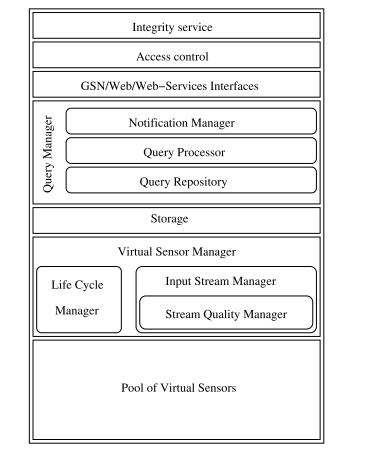
\includegraphics[width=0.8\textwidth]{Chap2/figures/gsn_arch.png}
		\caption{GSN Architecture \cite{F2006}}
		\label{bg:fig:gsn}
		\end{figure}

Figure \ref{bg:fig:gsn} outlines the architecture of GSN, showing that the virtual sensors are stored on a central node and their inputs are managed and stored. GSN also comes bundled with a web interface to show all active sensors and their most recent recordings, as well as the implementation of web services to access the data outside of the interface.

Data from virtual sensors pass through the virtual sensor manager to the storage layer. Once the data has been stored, the query manager is invoked and queries are loaded from the repository and executed by the manager. The results of the queries are then handled by the notification manager and also made available to the web interface. Notifications can be extended to support many different forms of communication, such as SMS, email or web services.

Virtual sensors do not natively support all hardware, although new virtual sensors can be described using XML, and there may be a need to implement an entirely new virtual sensor. In this case, technical knowledge is required, and new sensors can be implemented through use of the Java programming language. This provides more control over the use of XML and allows users to specify how sensed data is stored in a database, use external libraries to receive proprietary data, specify processing workflows before the data is stored or implement new notification methods for the users of the network.

To show the simplicity of a basic virtual sensor, \cite{Aberer2007} describes a temperature sensor that we reproduce here in Listing \ref{bg:lst:gsn:vsensor}. The file is human-readable and does not require specialist knowledge when compared with programming languages, with tags that have self-explanatory names. In this example, the output structure shows that only a temperature reading is received and that the data should be stored permanently. The stream source specifies the content of the stream and the query details the standard query that should be used to extract data from GSN.
\vspace{\baselineskip}
\begin{lstlisting}[caption={Example Virtual Sensor},label={bg:lst:gsn:vsensor}]
<life-cycle pool-size="10" />
<output-structure> 
	<field name="TEMPERATURE" type="integer"/> 
</output-structure>
<storage permanent-storage="true" size="10s" /> 
<input-stream name="dummy" rate="100" > 
<stream-source alias="src1" sampling-rate="1" storage-size="1h">
<address wrapper="remote"> <predicate key="type" val="temperature" /> <predicate key="location" val="bc143" /> </address> 
<query>select avg(temperature) from WRAPPER</query>
</stream-source>
<query>select * from src1</query> 
</input-stream>

\end{lstlisting}

The modularity and flexibility of GSN makes it different to existing middlewares as it has not been designed for any specific hardware and modules of the middleware can be replaced, such as the database. 

	\subsubsection{FACTS}
		One such example is the FACTS middleware, an approach that uses a fact repository to coordinate nodes. Rules can then be implemented to process sensed data and fired when certain conditions are met \cite{Terfloth2006}. More traditional sensor middlewares control the network and manage sensed data but this rule based approach allows for more flexibility, where rules can control the transmissions and process the data upon receipt.

		\begin{figure}[h]
		\centering
		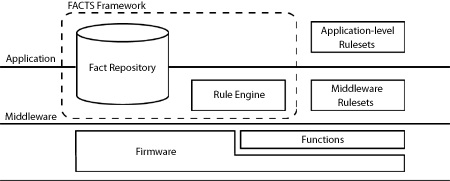
\includegraphics[width=0.8\textwidth]{Chap2/figures/facts_architecture.jpg}
		\caption{FACTS Architecturei \cite{Terfloth2006}}
		\label{bg:fig:facts}
		\end{figure}

		Figure \ref{bg:fig:facts} shows the FACTS architecture, with the middleware holding the rulesets and a distributed fact repository. Data within the network is stored as facts, providing a standard data format throughout the network and hardware abstraction. When new facts are received, ususally because of new sensing data, the rule engine checks to determine whether any rules should be fired. The ruleset definition language (RDL) is used here and each ruleset contains a group of relevant rules. Each rule is given a priority so that, if more than one rule is triggered by a fact, then the higher priority rules are fired first.

		Listing \ref{bg:facts:rule} shows a FACTS rule, written in Haskell, that determines which geographic areas are covered by nodes. The name of each rule has no prefix, statements are prefixed with `->' and conditions are prefixed with `<-'. The \textit{sendRange} rule runs after a timer expires and removes that timer. Lines 4 to 12 set a \textit{rangeFact} fact that contains the range it expects to be able to cover. The rest of the rule sends the fact to all nodes within range and sets a new fact to show that it has sent its range information. 

		The \textit(xyMinCovered) is a simplified rule that, upon receipt of range information from neighbouring nodes, checks whether the range of the neighbouring node overlaps with its own range and the final \textit{determineCoverage} rule then stores that coverage information in a fact as knowledge of whether or not it is the only node to cover a particular geographic region. This can then be used to inform future routing and sleeping decisions.
\vspace{\baselineskip}
		\begin{lstlisting}[caption={Coverage Algorithm in FACTS Rules}, label={bg:facts:rule}]
 sendRange
 <- Exists Timer.expiredSlot
 -> Retract Timer.expiredSlot 
 -> Define "rangeFact"
 -> Set ("rangeFact" "xMin")
	(posXSlot - System.txRadiusSlot)
-> Set ("rangeFact" "xMax") 
	(posXSlot + System.txRadiusSlot)
-> Set ("rangeFact" "yMin")
	(posYSlot - System.txRadiusSlot)
-> Set ("rangeFact" "yMax")
	(posYSlot + System.txRadiusSlot)
-> Send 0 System.txPowerSlot 
	("rangeFact" [(("rangeFact" "owner")
	== nodeIDSlot)])
-> Define "rangeSendFact"

xyMinCovered
<- Exists "rangeSendFact"
<- Eval ((posXSlot - System.txRadiusSlot)
	< ("rangeFact" "xMin"))
<- Eval ((posYSlot - System.txRadiusSlot)
	< ("rangeFact" "yMin"))
-> Define "xyMinCoveredFact" 

determineCoverage
<- Exists xyMinCoveredFact"
-> Define "coveredFact
		\end{lstlisting}

		While FACTS itself does not utilise any local knowledge, the repository is used as a source for all previously sensed data and would be an excellent source of knowledge to assist with the classification of future readings. Also, the ability to add new rulesets, without technical knowledge of the hardware of each node means that users of the network have the ability to add knowledge in the form of less technical, high-level rules.

	\subsubsection{ITA Sensor Fabric}
	The ITA Sensor Fabric is a collaboration project between IBM, the US Army and the UK MoD. Sensor Fabric, or Fabric, is a two-way messaging bus and set of middleware services connecting network assets to each other and users \cite{Wright2009b}.

The core difference between the Fabric middleware and others is that not every node is sensing all of the time, sensor nodes are tasked when there is a requirement and they stop as soon as that task has been fulfilled. Similar to sinks in a traditional WSN, Fabric utilises Fabric nodes, which run the following three pieces of software:
\begin{enumerate}
	\item Message Broker - Provides the communication infrastructure.
	\item Fabric Registry - Holds information about the current deployment, such as all nodes deployed, all assets, routing information and tasks. Deployed in the form of a database.
	\item Fabric Manager - The main service on the node to track the status of connected sensors, establish communication channels, provide a container for processing, plug-ins and to extends the capabilities of the Fabric.
\end{enumerate}

Fabric runs on a Publish/Subscribe model, a sensing requirement is sent to a messaging broker as a subscription and this is distributed through all Fabric nodes and, thus, all sensor nodes. Sensor nodes then publish their data and the relevant data is sent to all applications that have subscribed to the data. 

The plugin structure of Fabric makes it stand out from existing middlewares, allowing its functionality to be extended through web interfaces.

Because Fabric has been developed for military purposes that cross countries, policy enforcement has been implemented to restrict access to the granularity of sensed data but these access levels do not simply apply to a military context. Using our motivating scenario, researchers and professors should see animal images whereas the Sabah Wildlife Department should see images of hunters and people in the forest.

	\subsubsection{Sensor Web Enablement}
		The Open Geospatial Consortiums's (OGC) Sensor Web Enablement (SWE) is a set of standards to allow developers to make sensors and sensed data repositories accessible via the Internet \cite{botts2008ogc}. While this is not a middleware, these standards can work with existing middleware in order to publish their sensed data to the Internet. The SWE framework consists of:

		\begin{itemize}
			\item Observations \& Measurements (O\&M) - General models and XML encodings for observations and measurements.
			\item Sensor Model Language (SensorML) - Standard models and XML schema for describing the process within sensor systems.
			\item PUCK - Defines a protocol to retrieve a SensorML description and other information from a device, enabling automatic sensor installation, configuration and operation.
			\item Sensor Observation Service (SOS) - Open interface for a web service to obtain observations and sensor descriptions for one or more sensors.
			\item Sensor Planning Service (SPS) - An open interface for a web service that a user can determine the feasibility of collection data from one or more sensors and submit collection requests.
		\end{itemize}

		These components can be integrated into existing middleware, clients and sensors and not all need to be used, some middleware, such as MufFIN \cite{Valente2011}, have just used SOS and O\&M but 52North have devloped an open source implementations of all components of SWE \cite{broring2011new}.

	\subsubsection{Internet of Things}
		In \cite{giusto2010internet}, the Internet of Things (IoT) is described as the ``concept of pervasive things... which, through unique addressing shemes, are able to ineract with each other and cooperate with their neighbours to achieve common goals.'' The number of devices that are part of the IoT grows daily, from thermostats and smoke detectors \cite{nest} to activity monitors \cite{fitbit}. Some of these devices have their data siloed away and it is only accessible through a web interface or a mobile app, but most have an Application Programming Interface (API) that allows the raw data to be access and queried. Because of this, sites like If This Then That (IFTTT) \cite{ifttt} have been created to link together various services and use simple if statements to act on changes in the data. IFTTT uses \textit{recipes} that follow the rule of: \lstinline{IF Service1 changes THEN perform action on Service2}. For example, \lstinline{IF I take a picture using my phone THEN upload it to Twitter} or \lstinline{IF a new item appears on my RSS feed THEN add it to my reading list}. While, IFTTT is not a traditional middleware, it does monitor user's connected services, some of which may be sensors around the home or attached to their person.

		A more tradtional middleware for the IoT is Xively, a cloud platform that allows devices to upload their sensor readings to an endpoint and view readings from others \cite{xively}. Feeds can be public or private and Xively can be used with almost any Internet-enabled devices, such as webcams, temperature sensors or alarms. Other sites, such as Dweet.io \cite{dweet} and Open Sen.se \cite{opensense}, have also been in operation for a few years that provide a similar service to Xively. Open Sen.se combines the recipes of IFTTT with the storage of Xively to create a middleware that supports actions being performed when certain sensed data is received. For example, a temperature sensor could trigger an alert on Open Sen.se that would alert a user via e-mail, or through social media. This combination of devices with online services and applications allows a middleware to do more than simply store data, it can execute rules over the data, provide visualisations and create links between devices separated by hundreds, or thousands, of miles.


\section{Biodiversity and Environmental Monitoring Sensor Networks} \label{bg:bsn}
	In this section we will cover existing WSNs that are related to our motivating scenario or, more specifically, biodiversity focussed WSNs that have been deployed to monitor wildlife and/or the environment. WSNs for habitat, and wildlife, monitoring are especially important because these are areas that often need to be untouched by humans. Areas with high human disturbance can influence the abundance of species and some habitats, i.e. underground burrows, may be impossible to monitor without destruction. 
	
	One of the most well known WSNs to monitor habitat is the network deployed on Great Duck Island, an island off the coast of Maine, USA. A hierarchical network of 32 nodes was deployed to monitor a bird, known as the leach's storm petrel \cite{Mainwaring2002}. This network used a clustering approach for groups of nodes to send data to a gateway node, which would then route it back to the base station. The base station, located a few kilometres away on the island, has internet access and uploads the data to allow users to browse and process the data.

	A multihop approach was used here as they found that, for sufficient coverage, single hop connectivity would not cover all of the island. Acrylic enclosures were developed to ensure the nodes were weatherproofed for the conditions of the island, while maintaining the functionality of each sensor and not impeding transmission range. While the nodes, their casing and their sensors have been designed specifically for the deployment on Great Duck Island, the success of the network, running for 123 days in the early stages of WSN research \cite{Szewczyk2004c}, shows that this approach can be used elsewhere with similar effects; allowing hard to monitor and/or inaccessible areas to be continuously monitored.

	On a smaller scale, INternet-Sensor InteGration for HabitaT monitoring (INSIGHT) is a single-hop WSN that allows remote access for data and reconfiguring of nodes \cite{Demirbas}. Using off the shelf hardware, their findings show that their nodes could survive for 160 days on a single battery, supporting their claim that a single hop network allows for a longer network lifetime. 
	
	The key feature of this network is the ability for humans to remotely set reporting thresholds for sensor nodes. This means a user can prolong the lifetime of nodes by limiting the threshold they report on, as well as the fact that these thresholds are a way for users to add knowledge, albeit primitive, into a network.

	While there is research on cameras used to monitor animals \cite{Kays2009, Ahumada2011a}, these networks are generally cameras deployed with their memory cards manually retrieved and processed. In recent years, however, the use of wireless technologies and image-based WSNs has increased, \cite{Garcia-Sanchez2010b} uses wireless cameras to monitor the movement of animals between roads. Using commercial hardware and controlled sleep scheduling, this solution employs the use of nodes to detect movement and wake up more power-hungry camera nodes. While the nodes are wireless, the distance of the network from civilisation means that the data does still need to be collected manually and uploaded to a computer.

	Due to the advent of smartphones and tablets, as well as the improvements in 3G technology, projects taking advantage of more modern technologies have grown in popularity. Using 3G enabled cameras, \cite{ZSL} have deployed a number of devices in locations all over the world, such as: Kenya, Indonesia and the USA. The images captured are transmitted to a server and a website allows the general public to not only see the images in near real-time, but to classify the images as well. This crowdsourcing of collective knowledge lets people, that may not have domain knowledge, vote on an image and those votes are used to make classification easier.

	Over the past fifteen years, WSNs have grown from a concept to a real solution for monitoring the habitats, movements and eating habits of wildlife all over the world. Whether it is using GPS collars to monitor the movement of cattle \cite{Guo2006}, monitoring animal habitats on a remote island or using cameras to capture the animals themselves, the popularity of these networks has grown considerably and advances in technology have allowed these networks to be deployed in places that humans cannot access with ease.
	
		There are a number of situations where we may want to record data in an environment that is not safe for humans, such as a volcano \cite{Werner-Allen2006}, or that may be difficult for electronics to survive. In these cases, special considerations must be made during the design and deployment of the WSN, in order to ensure maximum  network lifetime with reliable readings.
	\subsubsection{GLACSWEB}
	Glacsweb is a sensor network to monitor the rate that which glaciers are melting. Deployed in Norway, specially designed sensors have been drilled into glaciers to monitor pressure, temperature, orientation and strain. Due to the high pressure and exposure to moisture, a polyester casing was used so that, once bonded, the node inside would be protected from its environment, but also preventing it from being recoverable.
	\subsubsection{Reventador}
	Volcano Reventador is in northern Ecuador and a WSN has been deployed on there to monitor eruptions. Similar to Glacsweb, weatherproof enclosures were used to prevent ash and moisture from breaking the sensors and long-range external antenna mounted to a pole was used to achieve communications over large distances when wireless communications have proven to be difficult \cite{Werner-Allen2006}.
	\subsubsection{Rainforest}
	There have been many studies on how the rainforest affects the range and quality of wireless links \cite{Figueiredo2009, Wark2008, Rahman2008}. In \cite{Figueiredo2009}, the humidity was shown to reduce 802.11 range by up to 78\% and \cite{Wark2008} explains that periods of rainfall reduce the link quality up to 100\% in some cases, resulting in the loss of a hop and this could prevent data from reaching the endpoint.


This section highlights the difficulties of deploying WSNs in harsh environments. Environments vary from freezing glaciers to humid rainforests to dry deserts with extreme temperature variation and the sensors cannot disturb their surroundings, be too conspicuous or require regular human attention that would disturb the area and affect the wildlife. 

\section{Local and Global Knowledge} \label{bg:lgk}
	The environment of a sensor network is rich and varied and we believe that knowledge of this environment and patterns in the data sensed can be used to inform the network on decisions surrounding the transmission and processing of newly sensed data. As our research began, we simply called this knowledge but, as our work continued, it became apparent that it could be catgorised further.

While we believe that we are the first to use the concept of local and global knowledge within the wireless sensor network domain, the terms have been around for many years. In 1999, a book that referred to local knowledge as \textit{indigenous knowledge} defined local knowledge as `systematic information that remains in the informal sector, usually unwritten and preserved in oral traditions rather than text' \cite{LadislausM.Semali}. 

Over the past twenty years, local knowledge has been used in various contexts, from researching lending and the credit market \cite{Stiglitz1990} to extracting local knowledge from natives to improve farming techniques \cite{DEWALT}. This research, as well as work that will be covered later, showed us that there are two kinds of knowledge: global and local. 

It was from agriculture research that we were able to refine our definition of local knowledge, \cite{Joshi2001} defines local knowledge as `knowledge that farmers have derived locally through experience and experimentation'. They also say that indigenous knowledge is different in that it is culturally specific. From this definition, as well as our work with our motivating scenario, we were able to generalise the definition and expand upon it.

We now define local knowledge as \textit{knowledge of an area, held by a domain expert, that has been gained through experience or experimentation}. This then means that global knowledge is \textit{knowledge of an area that can be accessed by anyone, without the need to visit the area directly}. The weather of a region is global knowledge because it can be found through a variety of media, whereas the saturation levels of the soil in a field would be local knowledge as it would require experimentation to gain that knowledge. Local knowledge could become global if it was readily available but some of these data are held in tribes of people without Internet access.

Using these definitions, we believe that \textbf{encoding local and global knowledge onto sensors can inform routing decisions to make better use of the bandwidth in resource-constrained WSNs by sending data that the node believes to be important first, rather than chronologically}. Patterns in the data, and knowledge of the environment surrounding a node, can allow a node to infer what data may be valuable, automate the processing of adding context to the sensed data, learn from previously sensed data and utilise global knowledge of ongoing projects within the network to determine what data is thought to be of a higher priority.

% \section{Relevant Existing Networks} \label{bg:rsn}
% 	In this section, we discuss existing networks that are related to our research question and/or motivating scenario. While most of the existing networks relevant to Danau Girang have already been covered in Section \ref{bg:bsn}, there are some WSNs that are not directly related to biodiversity but have been deployed in harsh conditions or involve interdisciplinary collaboration. Interdisciplinary networks are of particular interest because they include the crossover of specialist knowledge from two, or more, domains. For example, biodiversity networks combine computer networking and software development and bioscience while medical networks combine medical knowledge. This means that the networks must be developed with the operation of users that may not possess the same specialist knowledge in mind and, thus, need to be more generally accessible. These examples prove invaluable when designing our own WSN architecture as some middleware and hardware solutions have been created with ease of use as a priority and do not require technical knowledge, allowing them to be used with little training.

% \subsection{Context-Awareness}
% 	While standard WSNs have been prevalent for many decades, new research on the Internet of Things \cite{Atzori2010} has brought about interest in context-aware sensing, in some cases this is for small wearable devices to track fitness but the applications are much broader. Here we will look at WSNs that use context to make informed routing decisions, save power, or prioritise the transmission of data. We consider context-aware sensors the step before a network making use of local and global knowledge and the uses of knowledge in these scenarios will only enhance the data further.

	% \subsubsection{Health}
% 		Health monitoring is one of the more obvious choices for context awareness as classifying readings can often help determine the health of someone, rather than their self-reports. AlarmNet is a WSN that uses context to provide long-term health monitoring for people in assisted-living environments \cite{Wood}.
	
% AlarmNet employs context-awareness to learn about the activity levels of the patient and uses that knowledge to determine when changes in the readings may mean that the patient is at risk. Once the AlarmNet system has completed its learning period, deviations, from what it has recorded as the normal activities for the patient, are sent to nurses and doctors, with the idea that this information can assist with a diagnosis.

% As some nodes in the system will be battery powered, AlarmNet also employs a subsystem, called the Context-Aware Power Management System (CAPM), to control the power consumption of a device based on the recorded activities of the patient. The system uses policies, based on the context, to save power for all nodes in the system. For example, the system could put mains-powered nodes into a low-power state and disable all nodes outside of the bedroom when it detects that the patient has gone to sleep.

% This use of context has not only shown that it can assist with the lifetime of a network, but it can also provide valuable insight into sensed data to provide data enriched with semantics. AlarmNet is a particularly important example because of the learning period it employ, using a time period to add context to the sensor readings from a patient so that it is able to identify future activities that do not fit with the day-to-day pattens of the patient.

% 	\subsubsection{Wearable Devices}
% As wearable devices, such as the Fitbit and the Pebble smartwatch, are increasing in popularity, context-awareness is a useful tool to differentiate between the many activities that a person can undertake. The MObile PErsonal Trainer system (MOPET) is a wearable fitness devices that uses context to record data on jogging and fitness exercises \cite{Buttussi2008}. 

% While the project is five years old now, it is one of the earliest proof-of-concept devices created and shows how simple rules applied to sensor readings can be used to apply context. For example, the device consists of a GPS sensor and, when active, it is constantly recording positions. Using pairs of points, it is able to calculate the speed and, if the speed is consistent with jogging, then it records a running exercise.

% Fitness is not the only purpose for wearable computing, the eWatch is an early design for a \textit{smartwatch} that uses a microphone and light sensor to record the locations that the user visits, storing previous recordings in flash memory and matching them with current recordings \cite{Maurer}.

	% \subsubsection{UNETS}
	% 	*UNETS is tiered and context aware

\section{Conclusion}\label{bg:conc}
	In this chapter we have explored the components that make a WSN, as well as some existing deployments that are relevant to our motivating scenario. Sensor middleware have come a long way in the past decade and increased capabilities for sensor nodes have allowed for more intense processing to be carried out before any data is seen by a human. Context is now used on sensor nodes to infer the activity they are undertaking or even to determine when it should wake to sample. 

Local knowledge is not a new concept and it has been used for many years to extract information from indigenous people and in industry to adapt their processes to a local area, such as farming. However, we believe that our work is the first to apply local knowledge in the context of WSNs. Context-aware sensor networks have gone some way to support out hypothesis that some knowledge can increase the functionality of a network and enhance the quality of the sensed data, but we believe that the addition of LK and GK will only increase this functionality further.

The two primary components of a WSN that could be injected with local knowledge is the middleware and the routing protocol, each providing different benefits. Existing work has shown that the use of context-awareness in sensor middleware allows them to make dynamic, global changes to the network (Section \ref{bg:sm}), such as power management, whereas routing protocols affect the data that is sampled and sent to the endpoint(s) of the network, such as adaptive thresholds.

One issue in proving this hypothesis is the deployment of a network that utilises local knowledge. The deployment environment of our motivating scenario is not only interdisciplinary, it is in a region that is humid, dynamic and dense. Existing research has shown that the deployment of a WSN in these conditions means that range will be greatly reduced \cite{Figueiredo2009} and changes in humidity can prevent communication altogether, as well as moisture affecting the hardware itself.
To deploy a network, hardware must be adapted and the right medium must be chosen in order to maximise link quality and minimise dropped connections.

In Chapter 3, we describe how we used this research, along with our own findings, to choose suitable hardware for our network. As well as this, we used the results from previous rainforest range tests in the literature, to design  experiments that would aid us in choosing, and verifying, our choice of tranmsission medium.


\chapter{Technical}\label{chap:technical}
	In this chapter, we explain our motivating scenario in more detail, explore the sensor hardware that we researched and outline the results of experiments we undertook in the Malaysian rainforest. As highlighted in Section \ref{int:mot}, we have been working with Cardiff University School of Bioscience to design and deploy a WSN that utilises local knowledge, using an area of rainforest in Malaysia owned by the Sabah Wildlife Department, called Danau Girang.

The structure of this chapter is as follows. Section \ref{tech:motiv} explains what we aimed to deploy in Danau Girang and what our considerations were. Section \ref{tech:hw} introduces sensor hardware that is in use today and details the choices we made. Section \ref{tech:wireless} details the transmission medium choices we tried and also shows the results of experiments performed in both the UK and Malaysia. Section \ref{tech:sw} explains some of the software applications we developed in order to process sensed data on the nodes. Finally, Section \ref{tech:conc} summarises our findings and explains the choices we made for the sensor nodes we used in DG. 

\section{Danau Girang}\label{tech:motiv}
Based in Sabah, Malaysia, Danau Girang is a field centre located in Lot 6 of the Lower Kinabatangan Wildlife Sanctuary (LKWS), surrounded by secondary rainforest that had been logged up until the 1970s. Experiencing typical wet and dry seasons, the LKWS can receive more than 500mm of rainfall during the rainy season, dropping to lows of around 150mm during the dry seasons \cite{Walsh2009}, and up to 100\% humidity all year round. 

Danau Girang is uniquely situated in a rainforest corridor (figure \ref{tech:fig:map}) that joins two areas of rainforest together, with the corridor surrounded by palm oil on each side. Because of this, animals use the corridor to move between the rainforest regions and some use it to enter the palm oil plantation for new feeding grounds. This gives Danau Girang insight into the movement patterns of these animals in the corridor as well as in the rainforest itself, with a wide variety of species that are not commonly seen in other tropical regions of the world. Due to the remote nature of the centre, power is provided by a set of diesel generators which, typically, provide power from 10 am to 1 pm and 5pm to 11pm daily. Wireless Internet access is provided by satellite with speeds approximating 56k, although the upload speeds are considerably faster than downloads.

		\begin{figure}[h]
		\centering
		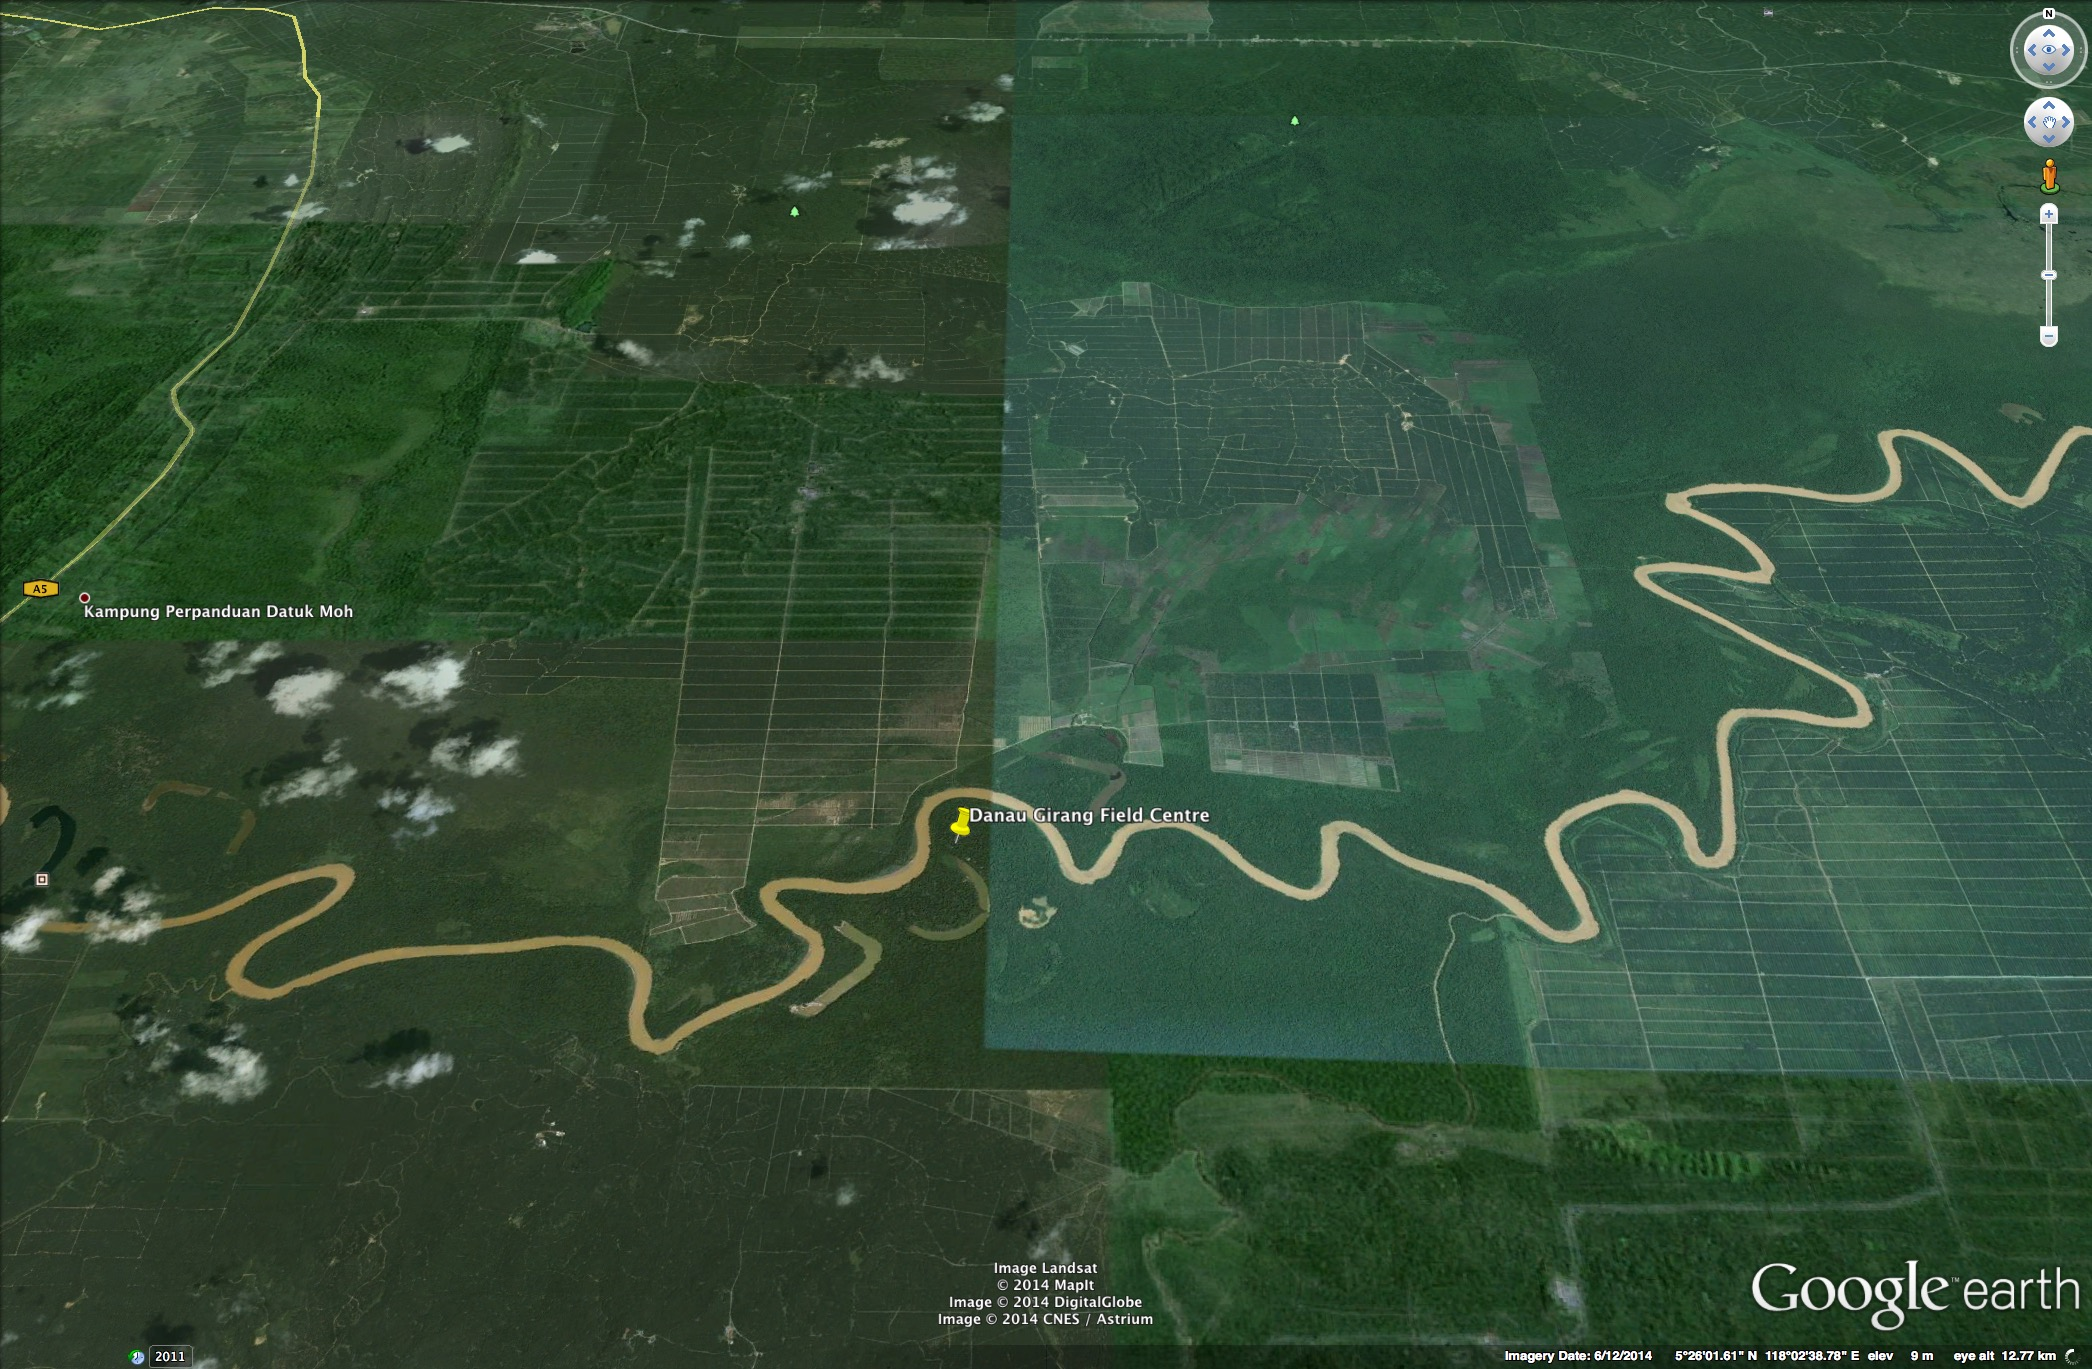
\includegraphics[width=0.8\textwidth]{Chap3/figures/dgmap}
		\caption{Aerial View of Danau Girang Field Centre}
		\label{tech:fig:map}
		\end{figure}

The corridor monitoring programme is a scheme that has been in place for more than five years, using wildlife cameras to track the movement of animals through the rainforest corridor and to capture species that are rare or unique to South-East Asia, such as the Bornean Clouded Leopard. Currently, Reconyx Hyperfire HC500 cameras are being used \cite{Reconyx}. These are standalone cameras that capture a user-defined number of images which are saved to an SD card. A trigger is caused by an infrared (IR) motion sensor when an object causes the IR beam to break. 

Images must be collected manually every two weeks from the cameras and the batteries are changed at that point as well, although a typical charge should last three months. The cameras are equipped with watertight casing but they are still exposed to moisture when the case is opened every two weeks and 100\% humidity seems to have an impact as well. Silica gel is used to prevent moisture inside the camera. We believe that humidity also reduces the battery life, as the charge drops from three months to around three weeks within the first few months of usage. However, the lack of constant power availability could also affect the charge of the batteries. Because power is not available all day, the batteries are charged for period of a few hours at a time. Not only does this reduce the number of charge cycles that these batteries can experience but it also means that they are never fully charged within one time period of power availability. Solar recharging is being researched to counteract this. Each camera is secured to a tree and more dangerous sites, such as known elephant paths, have protective cases as well. 

In 2010, twenty cameras were deployed for six month periods and then relocated based on the needs of the projects at that time. As of 2013, there are now ninety with a view to expand and dozens of projects within the field centre use the images gathered from these cameras. Initially, it was the job of visiting research students to collect the images but, since the number of deployed cameras has grown, full-time staff have been taken on to maintain them.

Our belief is that we can use the LKWS, and the locations of the existing cameras, to deploy a WSN that uses local knowledge gained from the researchers at DG to automate the collection of images, improve the battery life by not exposing the internals of the camera to the elements so often and, most important, prioritise the flow of data through the network by in-network processing. 
	
Annual visits, lasting three weeks, have been made to DG to test out hardware, software and wireless choices, in an effort to optimise the network. These visits have also been used to extract local knowledge from the area and researchers, by semi-structured interviews and watching them work.

\section{Hardware}\label{tech:hw}
	Before any visits were made to DG, meetings with staff members of the field centre were held in order to gain a better understanding of the environment and the project. This is where we were alerted to the humidity of the region and the fact that the failure rate of the Reconyx cameras has been as high as thirty per cent.

Reconyx cameras have no external interface support and the only way to access the images is through the removable SD card, because of this there is no way of attaching external sensor hardware to the existing cameras. In-network processing is an important requirement for our WSN and this did limit our choices to nodes that are computationally capable than more common sensors, such as the IMote 2 \cite{Nachman2008}.

In this section, we detail our research into suitable sensor hardware that met the following requirements:
\begin{enumerate}
	\item Able to perform processing of images and metadata
	\item Common interface availability (Serial, USB)
	\item Wireless enabled
	\item Battery-powered
	\item Expandable memory
\end{enumerate}
This section also details the modifications we made to any devices we tested in order to ensure they would survive in a humid environment.

\subsection{Pandaboard}

Texas Instruments supported the development of a reference Single Board Computer (SBC) that had specs similar to that of a modern smartphone and was capable of running desktop Linux, known as the Pandaboard \cite{instruments2012pandaboard}. A dual core 1GhZ ARM processor with 1GB of RAM, support for external storage, expansion ports, USB, Wi-Fi and Bluetooth in a board the size of two credit cards can be a powerful addition to a data heavy WSN, especially one that deals with images.

There is no mention of Pandaboards in the literature being used in WSNs but, the low power of the system and advanced capabilities, make it suitable for processing and transmitting data simultaneously. 
	
\subsection{IGEP v2}

The IGEP v2 is another ARM based SBC that uses a 1GhZ single core processor with 512MB RAM and similar connectivity features to the Pandaboard, but around half the size. This does result in a reduced power draw and the device is still capable of running desktop Linux.

Due to the smaller size, and easier commercial availability, the IGEP has been used as a sensor node to record, process and send readings from multiple devices, such as air temperature, GPS and oxygen saturation as part of environmental monitoring \cite{Resch}. In their research, they found that the IGEP achieved 9.1 hours of uptime using a 4000mAH battery, a capacity used in many modern smartphones.

\subsection{Waspmote}
The Waspmote is a general purpose sensing board that is designed to allow plug-and-play connectivity for multiple sensor modules. The node can be programmed with C++, using the Standard Development Kit (SDK) developed by the manufacturer. The processing power is not comparable to the more powerful SBCs, but the 600mAh battery is reported to last three months and the size is much smaller \cite{Lib}.

One of the benefits of the Waspmote is that they are commercially available with an actively maintained programming environment.

\section{Range Experiements}\label{tech:wireless}
	In this section, we explain the experiments we carried out to test the performance of different transmission media in the UK as well as the Malaysian rainforest. While range is the most important feature, a data rate that can handle hundreds of large readings in a day is a requirement. Our motivating scenario is focussed on the transmission of sets of 3 images for every trigger; where a sensor can trigger hundreds of times in a day.

\subsection{Wi-Fi}\label{tech:wifirange}
Wi-Fi was already available on our initial test platforms and the high data rate made it suitable for sending a large volume of images in a short period. We knew that current cameras deployed in DG were up to 1km apart and we did not expect to cover that range completely, but we did expect to achieve that coverage by using intermediate nodes.

Research, outlined in Section \ref{bg:trans}, showed that the rainforest could reduce the range by up to 78\% and the ideal maximum range of 2.4GhZ Wi-Fi is 100m \cite{Dhawan2007}. 

We tested Wi-Fi range using two IGEP boards, powered by 4 D Cell batteries and running a lightweight Linux operating system.	The IGEP nodes we used did not have any additional hardware and the nodes were tested without the use of an external antenna. A Java application was written to periodically scan for available networks and store those results in a text file. One IGEP board was set as the base station and attached to a tree, at the same height it would be if it was attached to a camera, and another was walked to specified points around the base station at defined locations. These locations were chosen to include as many distances as possible and as many different forms of obstacle between the searching node and the base station, such as: line of sight (LOS), medium vegetation or thick trees.
			
This experiment was run in a wooded area in the UK and in the rainforest at DG. The specified maximum range of 802.11g is 120m. When considering attenuation and obstacles we were expecting the signal to be reduced by up to 50\% in the UK. However, we found that we received a maximum range of 30m, with LOS. Figure \ref{cardiffsnr} shows the results we experienced, while testing in Cardiff, some of the drops in signal can be attributed to dense foliage and readings that were not LOS, but a maximum range of 31m, with an SNR of 29.5 dBm, is less than we expected, as the UK does not experience high humidity often.
			
			\begin{figure}[!t]
			\centering
			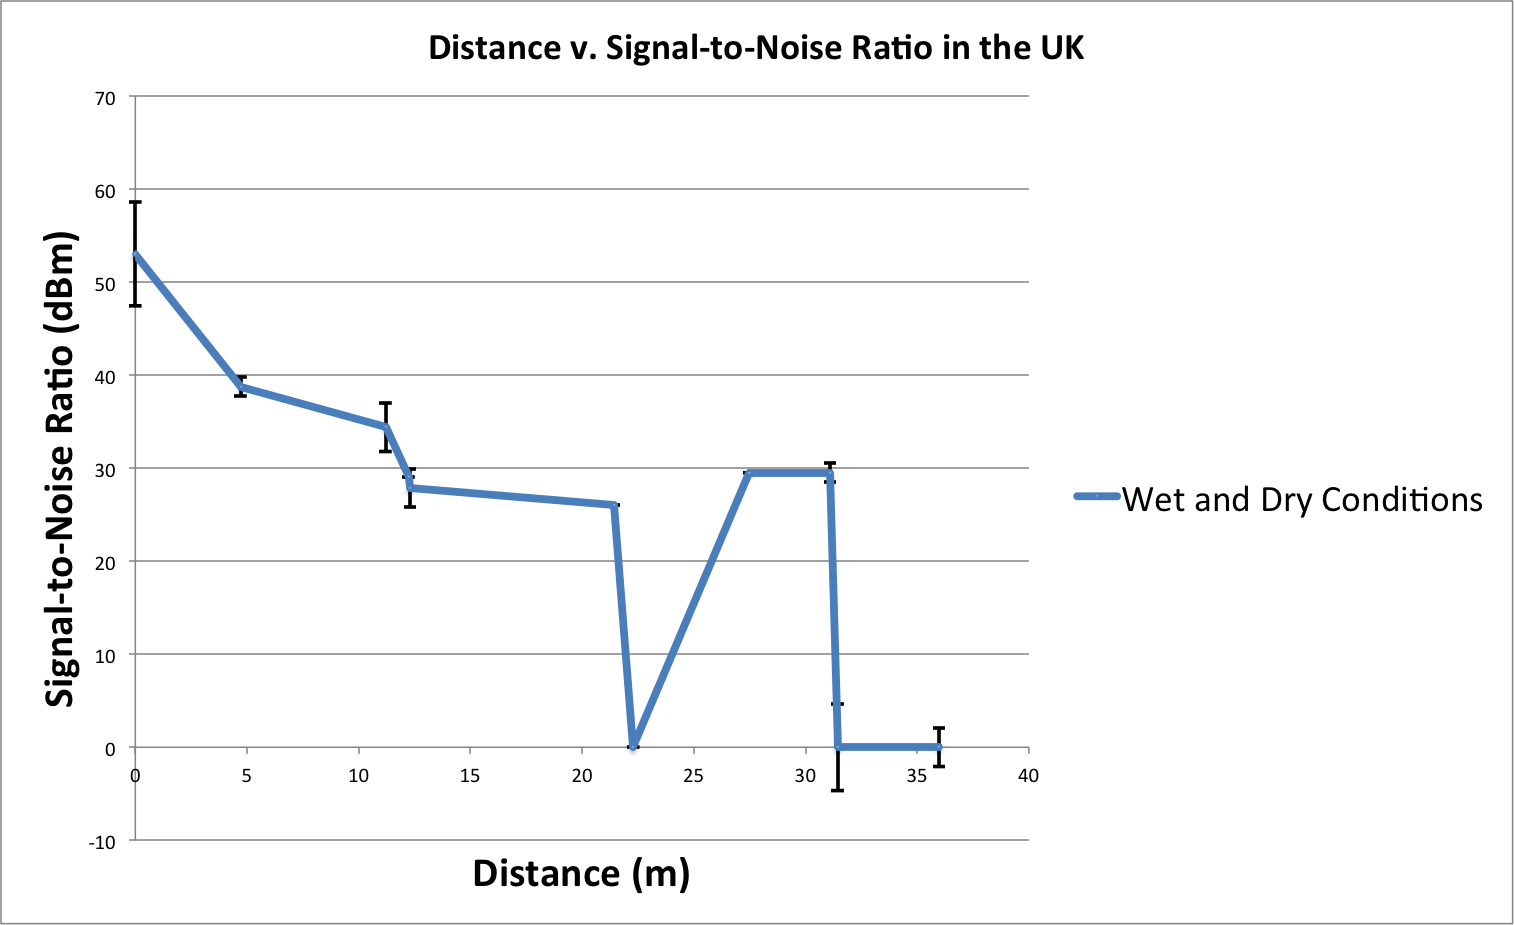
\includegraphics[width=0.65\textwidth]{Chap3/figures/bp_snr.png}
			\caption{Signal-to-Noise Ratio for Wi-Fi in UK Woodland}
			\label{cardiffsnr}
			\end{figure}
			
	The graph does show a drop at 22m, this was due to the dense foliage that restricted the LOS between the base station and the receiving node, with five runs of this test we observed the same results. The primary aim of this experiment was to prove the viability of Wi-Fi and to ensure our application functioned as intended, which it did. Further experiments could have been run to remove the anomaly but the results of the experiments in Danau Girang were the focus.
		 
	Despite the poor range from the tests in the UK, it was consistent with other studies reporting signal degradation of up to 78\% in areas with dense foliage. We visited Danau Girang in 2011 to gather the requirements of the network and ensure the hardware is able to survive the humidity. Range experiments were run in the rainforest to see if a more humid environment impacts range any further, Figure \ref{malaysiasnr} shows this.
			
			\begin{figure}[!t]
			\centering
			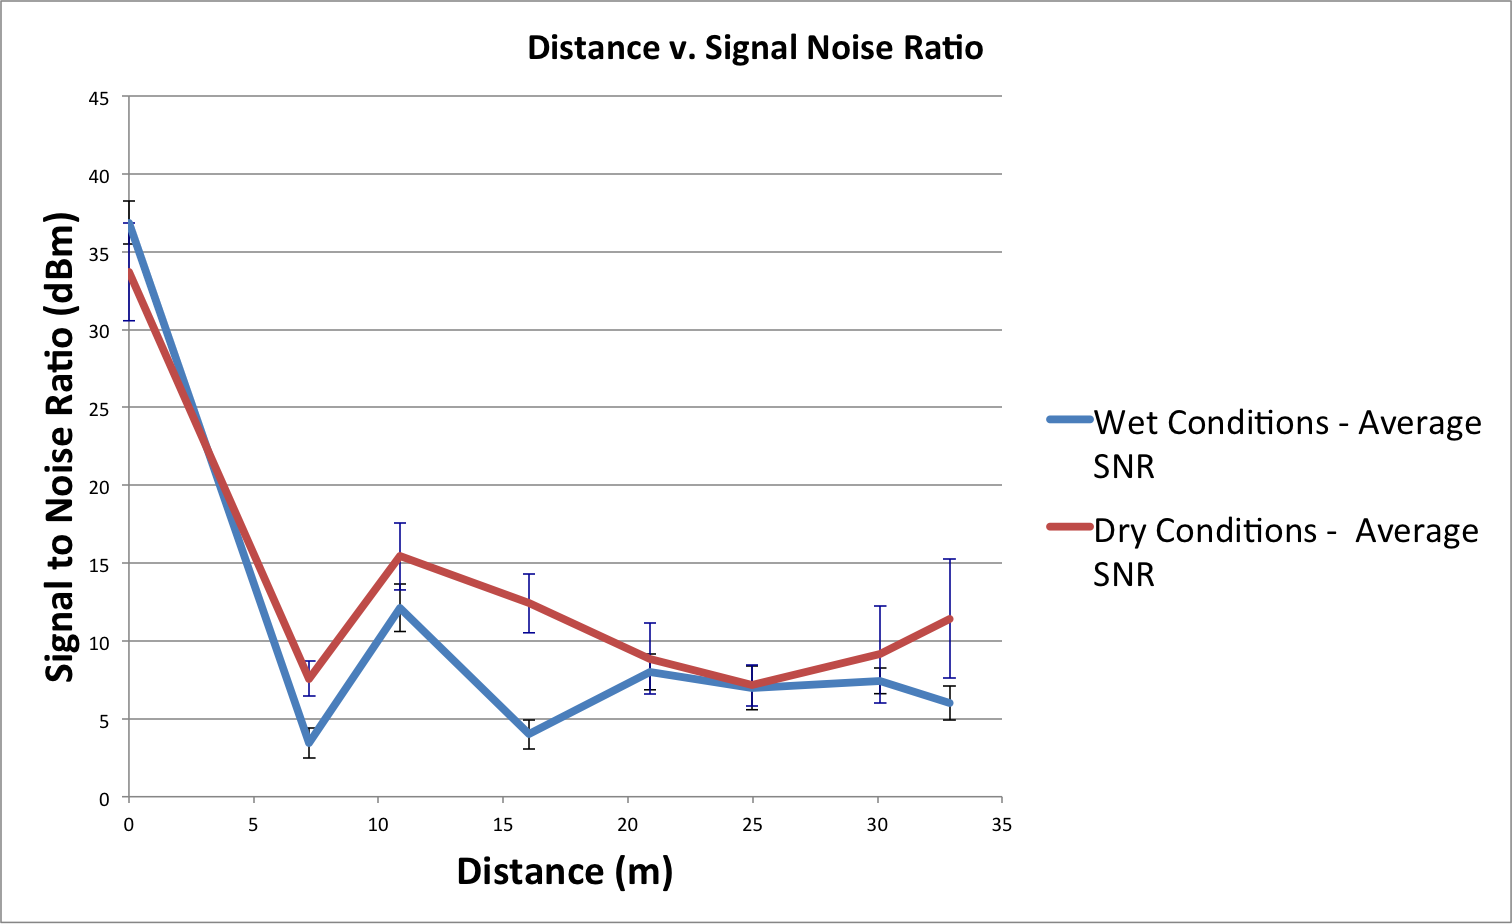
\includegraphics[width=0.65\textwidth]{Chap3/figures/dg_snr.png}
			\caption{Signal-to-Noise Ratio for Wi-Fi in Malaysian Rainforest}
			\label{malaysiasnr}
			\end{figure}
						
			Comparing figures \ref{cardiffsnr} and \ref{malaysiasnr} shows that the maximum distance to receive a signal is approximately the same in Malaysia as it is in the UK.  There are more signal drops but this seems to be due to denser foliage blocking the line of sight. However, it does suggest that the humid environment of the rainforest does not have a significant impact on the received signal. It is clear that the denser rainforest does impact the signal-to-noise ratio in a much shorter distance from the base station but a link is still made, allowing for a successful transmission of data.
			
Due to the poor results of these experiments we researched alternative methods to increase the range without impacting the environment the network is to be deployed in. We considered using intermediate nodes, not attached to cameras, to account for the lack of range but, because some cameras can be up to 1km apart, we would need more than 30 nodes to create a connection between two locations.
			
We also researched wireless technologies that are more common in sensor networks. This does mean that the data rate is not as high as Wi-Fi and error correction in packet streams is not always as robust, but it is more suited to sensor networks, using less power and providing longer range.
			
Finally, we considered using the researchers or animals at Danau Girang, as `data mules', creating temporary links between nodes while they are in the forest. However, the trip to Danau Girang yielded the information that researchers generally do not cover those distances in the forest and data delivery would be sporadic.
			
Although the range of Wi-Fi is poor, for our requirements, in both Malaysia and the UK, it did show that the results we experience in the UK are very similar to the results in Malaysia. This means that tests run in the UK should be indicative of what we can expect in Danau Girang.

\subsection{DigiMesh}\label{tech:digimesh}
		Due to the poor range results of Wi-Fi, we created a second prototype of the network, using DigiMesh. DigiMesh is a proprietary wireless protocol, based on the 802.15.4 standard and designed for devices with limited power. Using the same frequency as Wi-Fi, DigiMesh has been reported to provide 7km of range, with a data rate of 250kbps.
		
In our prototype implementation, we are using Waspmote sensor boards \cite{Waspmote}, a general purpose node that is capable of transmitting through various communication mediums. Our Waspmotes are provided with DigiMesh modules and a 2GB SD card to store sensed data.
		
When testing the range of the Waspmotes, we followed a similar method to that which is outlined in Section \ref{sec:wifirange}. One board is in a fixed location and running a C++ application to poll for nodes in the network. Once a node is found it sends a message to the node every 10 seconds. The second board is set to scan the network and receive packets as soon as a base node is found; this node is then moved to different locations.
			
The receiving node prints out variables related to the received packet, such as: Received Signal Strength Indicator (RSSI), source MAC address and packet ID. However, not all packets are received so the RSSI can display 0 if there are errors reading or if packet collision occurs. We found this to affect the results and have just used the two nodes to identify the maximum distance they can be apart, while maintaining a stable connection.
					
Initial experiments were run in a moderately vegetated area in the UK which yielded 497m of range. Limitations with buildings preventing us from testing any further but the signal strength still proved to be strong.
			
The initial results for the range tests proved positive and DigiMesh does seem to be a viable solution to account for the lack of range when using Wi-Fi. As the frequency is the same as 802.11g, thus licensing it for worldwide use, we expected similar results in Danau Girang..
						
Experiments were run in 2 areas of the rainforest around Danau Girang and the results yielded were not the same as we experienced in the UK, and thick vegetation proved to have a significant impact on the range, reducing it by almost 50\%.
			
In more open areas of the rainforest, we achieved 199m on average, more dense regions of the forest reduced this to 102m on average. While these results are not as high as we achieved in the UK, they are still suitable to use DigiMesh in the deployment of a WSN. This could be because we were using low-gain antennas and little configuration had been made on the DigiMesh radio.

\subsection{Adapting for Harsh Environments}
	All of the hardware that we used for experiments had their components exposed and would have become compromised if moisture came in contact with them. To protect them from this, we used waterproof cases with a protective foam inside, known as Pelican cases, to keep the nodes watertight, but still allowing airflow to displace the heat generated, shown in Figure \ref{fig:tech:pelican}.
	External antenna can be fed through the lip of the case, using thin cable, ensuring that the range of the transmissions is not affected by the case. 

			\begin{figure}[h]
			\centering
			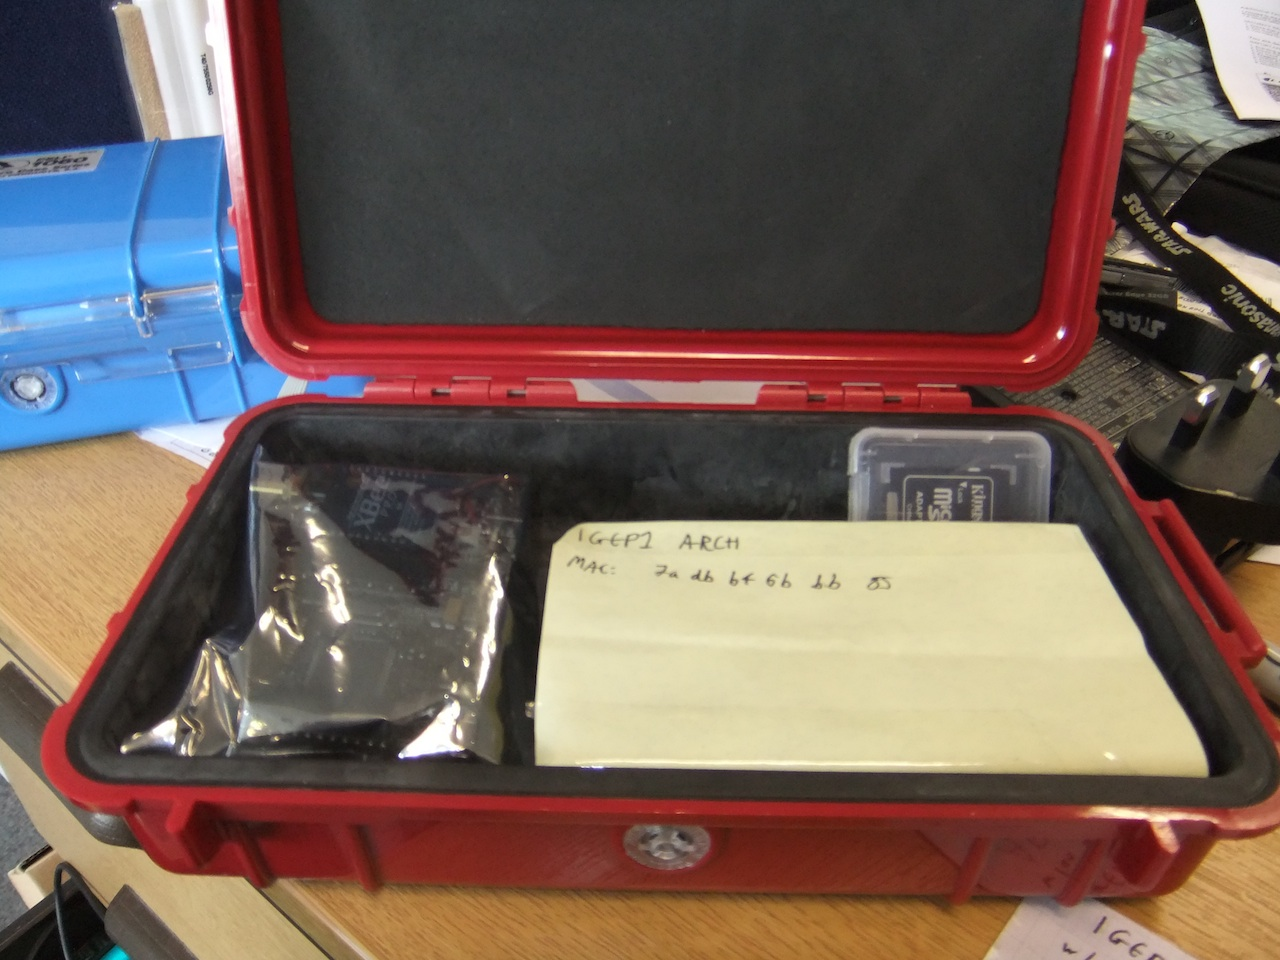
\includegraphics[width=0.45\textwidth]{Chap3/figures/pelican}
			\caption{Pelican Waterproof Case}
			\label{fig:tech:pelican}
			\end{figure}

\section{Software}\label{tech:sw}
	In this section, we explain the image processing software we developed for the real time processing of images within the network, as well as the retrospective processing of images that has been taken during previous deployments.

	\subsection{Triton} \label{tech:sf:triton}
		Triton is a C++ program that makes use of the Open Computer Vision (OpenCV) library for performing popular image processing functions. Triton takes in a set of images, combines them and builds a background model. Using this model, the foreground is extracted from the image and this is scanned for objects. If an object is found, it is extracted to a separate and saved as a black and white template, to minimise space and assist with future classifications.
		
		Primarily, we developed this tool to detect the large number of empty images captured around Danau Girang, due to trees falling, movement of the Sun, fast animals or dirt on the lens. However, Triton proved to be quite effective when finding images of interest and it was modified to be used with our sensors. In this section, we explain how Triton was tested and compared with human observations. To ensure a valid comparison, we also compared both results to a random classifier.
	
		During a typical three month deployment along the Kinabatangan River more than 40,000 images can be taken. A large proportion of these images can be classed as \textit{false triggers}; which are images captured by movement detected with the motion trigger of a camera when there is no object of interest. These can be caused by changes in the light, falling trees or animals moving too fast.
		
		Using the images, taken in sets of three, and separating the images taken by specific cameras, we build a Gaussian background model and used that to detect animals in the foreground, classifying the detected foreground as the ROI, and extracting it.
	
		As mentioned in Section \ref{sec:scenario}, Figure \ref{origimg} shows an image taken by a wildlife camera. The dynamic background and light levels should be noted here. This image is number 1, in a set of 3, a background model is built from these images and added to the pre-existing background model built by that camera. The foreground of the image is then extracted and ROIs, larger than a threshold, are identified. The largest ROI is then extracted from the image and saved separately.
	
		From our visit to Danau Girang in 2011, we collected images from two different three month deployments, in two different lots in Danau Girang, giving us just over 70,000 of images to test our approach. The images are sorted by the camera and the date of collection. We process every 3 images as one set, building a background model of all three images.
		
		We manually processed all of the images initially, marking images that are empty as false triggers. We then processed the images, using our application, and a resulting processed image is created from every set of 3 images. If nothing is detected in a set then no image is created and that set is logged as empty. 
		
		There are four classifications that can be made with images sets:
		\begin{description}
			\item True positive: An ROI is extracted that contains the animal in the set.
			\item False positive: An ROI is extracted that contains nothing of interest.
			\item True negative: A camera is triggered with nothing of interest in the image and no ROI is extracted.
			\item False negative: An image with interesting contents has no ROI extracted.
		\end{description}
		
		The processed images are then compared with our manual findings. The accuracy of our application is calculated by the following equation:
		
		\begin{equation}Accuracy = (T_{p} + T_{n})/Total Sets\end{equation}
		
		Where T$_{p}$  is the number of true positive sets extracted and T$_{n}$  is the number of true negative sets.
		
		Table \ref{table:processing} shows experiments run on a camera deployed in Danau Girang, testing on 300 sets of 3 images. These images were manually processed and classified as interesting or empty, of the 300, 94 sets were identified as interesting. Using Triton, 53 of those interesting sets (\textit{true positives}) were extracted, with another 17 \textit{false positives} extracted. 201 \textit{true negatives} were correctly identified and a further 5 were identified as \textit{false negatives}. 
		
		Out of the 94 interesting sets, 77 were identified correctly, giving an accuracy of 82\% for finding sets of interest. Furthermore, of 206 empty sets, 201 were found, which gives a 98\% accuracy at finding empty images.
	
		These preliminary results show that our method is effective at detecting false positives but is less effective at detecting false negatives. It appears that these misclassifications primarily come from black and white images taken at night, images where minimal movement of the animal has caused a trigger and images where an animal has caused a trigger but it has been too fast moving to be in the second two images.
		
		After a longer deployment, we would be able to build up a more substantial background model to account for some of the animals being less dynamic in images and we expect this to decrease our error rate thus reducing the number of false negatives. 
		
		\begin{table*}
			\hfill{}
			\begin{tabular}{|l|l|c|c|c|c|}
				\hline
					True Positive & True Negative & False Positive  & False Negative & Total Image Sets \\
				\hline
					77 & 201 & 5 & 17 & 300 \\
				\hline
			\end{tabular}
			\hfill{}
			\caption{Classification Results}
			\label{table:processing}
		\end{table*}
		
		The results of Triton were compared to a random classifier, implemented in Python. Table \ref{table:random} shows the outcome, with 72 \textit{true positives} extracted, resulting in an accuracy of 80\%. 73.3 \textit{true negatives} from a total of 206 were found, giving an accuracy of 36\%. Although this set does not compare to the number of images collected in a six month deployment, human classification is a time consuming process and to have 900 classifications is complex. Although these could be crowdsourced, the reliability becomes questionable, in part due to the specialist nature of the images. This does show that our approach is quite close to the accuracy of a human when finding images of interest, but is able to do so in a fraction of the time, processing hundreds of images every minute. 
		
		Triton, coupled with a set of human eyes at the heart of the network, should prove to be an effective approach for prioritising images through the network, even when a classification cannot be made through the use of local knowledge. More importantly, in an area where the environment is as dynamic as the Malaysian rainforest, 97\% accuracy for detecting empty images can be crucial, if only for saving network bandwidth.
		
		\begin{table*}
			\hfill{}
			\begin{tabular}{|l|l|c|c|c|c|}
				\hline
					True Positive & True Negative & False Positive  & False Negative & Total Image Sets \\
				\hline
					72 & 73.3 & 78.3 & 75.3 & 300 \\
				\hline
			\end{tabular}
			\hfill{}
			\caption{Random Classifier Results}
			\label{table:random}
		\end{table*}			
			%END OF INSERTION
%	
%	\subsection{ODACH}

\section{Conclusion}\label{tech:conc}
	In this chapter, we have shown the current hardware choices available for more computationally capable sensors and detailed our experimental results on how rainforest environments impact wireless transmissions. Although wireless technologies such as Wi-Fi provide a high data rate, their range is limited and not suitable for sparsely located nodes covering a large area; especially in a humid environment.
	Newer wireless technologies, designed for long-range communication in sensor networks, are becoming increasingly more viable and, while they do have lower data rates and less robust protocols, they are more suitable for a resource constrained WSN that requires minimal power draw when transmitting. 
	Using general-purpose hardware also means that there is no protection against water, humidity and animal or human intervention. We have adapted existing waterproof cases to suit our needs and preliminary short term deployments have shown that they are able to prevent any moisture from entering the case.
	 
\chapter{Wireless Sensor Network Architecture Design}\label{chap:arch}
	In this chapter, we explain our proposed network architecture that uses local and global knowledge to make informed routing decisions and to classify sensed data within the network. Our approach, K-HAS, uses a three-tiered, hierarchical approach with each subsequent tier providing increased knowledge processing capabilities. 

	We aim to show that sensors capable of processing knowledge will provide a more efficient network and be able to prioritise the delivery of interesting sensed data. We also believe that human input is a valuable way for such a network to learn about classifications it has made correctly, and incorrectly, and use that knowledge to inform future classifications. To prove this, we have developed an architecture that uses different levels of knowledge processing throughout the network, the Knowledge-based Hierarchical Architecture for Sensing (K-HAS).

	The rest of this chapter is structured as follows. Section \ref{arch:khas} outlines the main aims of K-HAS and what it is capable of that typical sensor networks are not. Section \ref{arch:tech} details the software and data standard choices we made for our implementation of K-HAS. Section \ref{arch:walk} provides a sample walkthrough of K-HAS, relating to our motivating scenario and Section \ref{arch:conc} concludes the chapter.

	\begin{figure}[h]
			\centering
			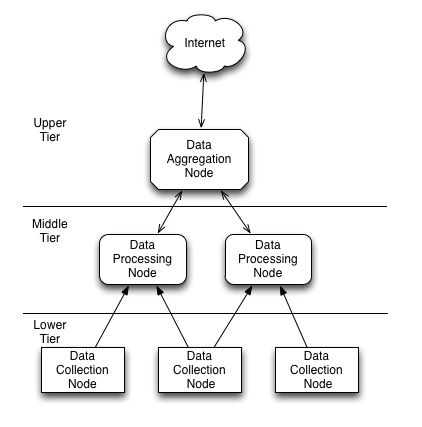
\includegraphics[width=0.65\textwidth]{Chap4/figures/khasarch} 
			\caption{Overview of the K-HAS Architecture}
			\label{arch:khas:arch}
			\end{figure}


\section{The Local Knowledge Problem}
While large in size, it is typical that a WSN would use low cost nodes with limited power, memory and computational capabilities; causing them to lack the ability to be aware of their surroundings or the data that they are sensing \cite{Akyildiz2002}. This means that, unless fixed by a routing protocol or a technician, data is delivered on a chronological basis and is then filtered at the base station, usually manually. Some WSNs store all of the data on the node and users of the network use a `pull' model to query for data from nodes \cite{Sadagopan}, but this requires some technical knowledge and, although it does increase the battery life of the nodes, it is a manual process again.

The environment that a WSN is deployed in is often a rich source of data to be sensed (such as inside a bird's nest to sense temperature, humidity and movement), which often contains patterns that can be used to improve the performance of the network. For example, if a node knows that it is has only been triggering between the hours of 6pm and 5am for the past few weeks, it can then learn to enter a deep sleep outside of those hours or use that time to transmit data it has been storing while it assumes it will be inactive, based on previous days. Alternatively, this knowledge can be used to prioritise data throughout the network so that the most important data is received first, instead of the most recent. An example of this could be two camera nodes deployed facing the entry and exit of a building, tasked with looking for intruders between 5pm and 8am. If the camera facing the exit is triggered at 5:01pm and the camera on the entrance is triggered at 5:05pm, then the knowledge that the security guard leaves through the exit between 5:00pm and 5:08 pm will allow the entrance camera to prioritise its capture as more important, as it is an irregular occurrence.

This knowledge can be categorised as either \textit{local} or \textit{global}. Local knowledge \nomenclature{LK}{Local Knowledge} is the knowledge of an area that has been gained through experience or experimentation \cite{Joshi2001} For example, a native to the Amazon may know that three of the locations in which the nodes are to be deployed are flooded for two weeks of the year, rendering their readings useless for that time period and increasing their risk of failure. This is local knolwedge, as it cannot be gained without experiencing the flooding in that area, or measuring local water levels.

We believe that the use of this knowledge can increase the effectiveness of the network, as well as prioritise data based on its value as opposed to when it was recorded. To show this, we have developed a network architecture for WSNs that utilises knowledge from the data it senses, as well as its deployed environment. It is called the Knowledge-based Hierarchical Architecture for Sensing (K-HAS) \nomenclature{K-HAS}{Knowledge-based Hierarchical Architecture for Sensing} and this thesis will show how K-HAS addresses the problem of delivering the most important data first and improving the overall efficiency of the network.

	
	\section{K-HAS}\label{arch:khas}
		K-HAS has been designed as an architecture for WSNs that addresses the above problem by using knowledge to classify sensed data and adapt to changes in the structure of the network. By pushing knowledge bases out to the edge of the network, all nodes in the network have some awareness of the data they are sensing, as well as how important it is, based on the current projects that the network is involved in. This is achieved by using rules with different levels of granularity based on the knowledge processing capabilities of that tier. Figure \ref{arch:khas:arch} shows a high level overview of K-HAS, showing the flow of data from each tier.
	
	
	\subsection{Data Collection}\label{khas:dc}
	The data collection (DC) tier is very similar to sensor nodes commonly used in a WSN, using hardware that has similar, limited processing power and storage to nodes such as: the I-Mote and Waspmote. These DC nodes are deployed at the edge of the network and tasked with sensing their environment, pre-processing the sensed data and using each other to relay data to the next tier.

	DC nodes are capable of performing processing on data, such as the time it was recorded and its size, but their limited knowledge processing capabilities allow them to have an increased battery life and reduced size, making them suitable for a variety of deployments as they can be integrated easily with existing devices (i.e. cameras) and be easily disguised, or hidden.

	\subsubsection{Knowledge Base}
	Reduced knowledge processing capabilities and low memory restrict the knowledge that these nodes can hold and they are limited to a static knowledge base that is encoded at the time of 	deployment. DC nodes run an operating system designed for embedded devices, the size of the operating system is minimal when compared to an operating system used on modern desktop computers and provides much more limited functionality, such as sleep scheduling, basic filesystem access and the capabilities to run a variation of popular languages. 

	For example, TinyOS \cite{levis2005} is an operating system designed for sensor nodes and uses a dialect of the C language, called nesC, that is optimised for the memory constraints of most sensor nodes. The operating system exposes components that allow basic commands, such as reading from the sensor interface or sending a message. Commands are executed as a request to perform some action and events signal the completion of that action. Intensive tasks, such as data processing, can be scheduled to run at a later time, ensuring that the low-power node remains responsive and preventing any calls from blocking other events.

	The Waspmote nodes, explained in Section \ref{tech:waspmote}, do not run any operating system and any event handling, networking or memory management is performed solely by the single file application that is uploaded to the node through the bootloader. Performing intensive tasks, such as local data processing, can drain the battery of the node, cause it to fill the available memory or even cause the node to go down. DC nodes do not have the safeguards in place that most operating systems and applications do, operational code must be lightweight, responsive and ensure that events do not run for longer than intended. 

	Some nodes within this class do not have the capability to process text files within the file system and, therefore, must have the knowledge added to their operational code. DC nodes only perform simple operations on the properties and content of the data that they sense, such as the time it was recorded, the location and its size. For more complex data, such as images and video, DC nodes do not possess the computational power required to process them and instead use the metadata associated.
	Unlike modern rule engines, these static rules do not use forward chaining and the outcome of one rule does not cause the rules to be fired again. Listing \ref{kb:dcrule} shows an example of some of the rules in the knowledge base and highlights that the core structure of this file is simply a list of if statements that can be executed one after the other. Forward chaining is not used here because processing times need to be kept to a minimum and a chain of rules being fired could easily overwhelm the node. If any rules are fired that suggest the observation may be interesting, it is prioritised through the network and potential classifications are encoded within the observation before it is sent on.

\begin{lstlisting}[breaklines=true, caption={Pseudocode DC Node Rules}, label={kb:dcrule}]
if month of observation is JUNE AND time of observation is between 17:00 and 19:00 and active otter project is TRUE
	add classification to observation(`Potential Otter sighting')
	prioritise observation as interesting
if temperature is 37 AND time of observation is between 01:00 and 05:00 and active leopard project is TRUE
	add classification to observation(`Potential Leopard sighting')
	prioritise observation as interesting
\end{lstlisting}

When the data is recorded by the DC node, the knowledge base is fired and inferences are made about the contents of the data. Each DC node has a static knowledge base loaded onto it before it is deployed, which is based on the local knowledge of the area that it is to be deployed in.  For example, a node deployed on the bank of a river would have a different knowledge base to a node deployed in the fields of a plantation.

Once a trigger has been processed, the data is packaged and then sent on to the Data Processing (DP) node.

	\subsection{Data Processing}\label{khas:dp}
	DP nodes act as cluster heads of the network, serving a subset of all deployed DC nodes. When data is sensed, it is forwarded through all DC nodes to the DP node that is tasked with serving the originating DC node. These nodes have more knowledge-processing capabilities than a DC node and do not perform any direct sensing. 

	Due to the greater capabilities, DP nodes have a much shorter battery life than DC nodes and a network typically consists of fewer DP nodes. These capabilities, such as increased memory and higher processing power, allow DP nodes to run a rule management system (such as Drools \cite{proctor2005drools}), that would not be possible on nodes that run on an OS for embdedded systems, that is able to handle more complex rules and process more than just files, they can perform the same tasks as most modern computers, such as: image processing, audio processing or reading metadata from files that requires extra libraries. When a DP node receives data, it processes everything associated, this includes metadata, the data itself and the inferences made by the DC node. If the DC node has inferred that the data is of a higher priority, then this data is processed first. This is done by prioritising the data at two stages: once it has been received and when it is about to be sent.

	In our current implementation, DP nodes use two different radios, a Zigbee radio to allow long range communication from DC nodes and a Wi-Fi radio that provides short range communication that allows for higher data rates.

	\subsubsection{Knowledge Base}
	In our motivating scenario the network is image-based, this means that the DP node would perform image processing, as well as processing the image metadata. The increased knowledge processing capabilities allow DP nodes to run rules dynamically, learning from the sensed data and providing classifications that change based on changes in the environment. For example, if a DP node has not seen an elephant before, and it is not aware of the object in the image, then it will await a human classification. The node will then record the time period that it receives elephant pictures, i.e. June to July, and become more alert the following year. Similarly, the node will know not to look for pictures of nocturnal animals during the day. This local knowledge allows processing power to be saved and, thus, time; this ensures that the processing of sensed data is optimised as much as possible in order to reduce the time it spends in the network.
	
	% The rule engine used in our current implementation is Drools, a Java based rule engine that allows for rules to be defined in \textit{.drl} files and these can be loaded dynamically into a knowledge base. This flexibility allows to be changed on the fly without the need to restart the device, or even require human access, as all of this can be achieved through network communication. 
	The rule engine used should allow for rules to be dynamically inserted into the rule base, so that rules can be updated through network communication.

	Upon receiving sensed data from a DC node, the rule base is fired on the metadata of each file received. If the rules determine that the data is of interest or, in the best case scenario, provides a classification, then the data is packaged and sent on to the Data Aggregation (DA) node.
	
	\subsection{Data Aggregation}
	Placed at the root of the network, these are nodes with the same knowledge-processing capabilities as DP nodes (although they typically have greater memory, processing power and a continuous power source) and would be accessible by users of the network. When DA nodes receive sensed data, it is unpacked and stored with a link to the node that the data originated from. Compared with a standard WSN, these nodes can be compared with a base station, or endpoint.
	
	Any information added by the DP node is parsed and classifications are extracted. If a classification is found, it is stored and the DA node checks for any active projects that contain the classification. If a match is found then all users involved in the project are informed via their preferred method of communication. Using the motivating scenario as an example, the people involved with projects could be researchers and professors and they may be looking for images of leopards, requesting to be informed via Twitter.
	
	All sensed data received, regardless of whether it has been classified, is accessible through a web interface hosted by each DA node. The interface shows all of the sensed data from each deployment, along with the associated classification. More importantly, it allows users to classify the data using a voting system. Users have roles which give them different privileges within the system. Normal users are able to vote and the majority vote is seen to be the current classification. While this is not a necessary feature of a DA node, it does allow the network to utilise the knowledge of human experts to inform future classifications.
	
	However, privileged users are able to confirm a classification and prevent any further votes. Once a classification has been confirmed, it is then sent back to the DP node it originated from. If the classification made by a user is different to the one inferred by the node, then it updates its knowledge base and acknowledges receipt.

	This system is vital in the early stages of deployment as this is used to build up a knowledge base. The more user classifications there are, the more accurate the network will be in the future. After a few months of classifications, K-HAS is then able to use the knowledge base to make more informed classifications, requiring fewer classifications/confirmations from users. The exception to this is sensed data that cannot be matched to the knowledge base.
	
	\subsubsection{Knowledge Base}
	DA nodes do not typically experience the resource constraints that DC and DP nodes must compensate for. Because of this, they hold a global knowledge that contains a history of all observations made by all nodes, as well as the location and deployment times of all nodes in the network. When nodes are deployed, this is updated, by users, to show the location of the node and when it was placed. 

	Every classification sent from DP nodes is stored in a database and contains all information about an observation: date, time, originating node, route taken within the network, location, sensed data, classification of sensed data. They also hold information for all projects running, for example: a project to track elephant movements within the forest. When sensed data that could be related to the project is received, such as an image with an elephant classification, users associated with that project are informed through email, or other means.
	
	While DC do not store any of the observations they capture, and DP nodes only store part of the observation that can be used in future classifications, DA nodes store the complete observation made by every DC node, as well as any extra knowledge that is added by users upon receiving the sensed data. What is stored by the the DP node is dependent on the deployed purpose of the network. For example, in our motivating scenario, we store: the processed image, the classification, the node it originated from and the date and time it was captured.
	
	As well as this, the functionality of DA nodes can be extended to provide administrative operations on the network, such as the recording of node locations, time of deployment and viewing all active nodes. This allows the DA node to monitor active nodes and alert users if a node has not sent any data in a while. The longer a K-HAS network runs, the more knowledge a DA node gains, both from users that classify observations and from changes in the sensed data. This knowledge is then relayed back to DP nodes, updating their knowledge bases as to what clasifications were correct and which need updating for future observations.

	\subsubsection{Feedback Loop}
	The feedback loop is a protocol within K-HAS, that uses human input, and other sources, to update DP nodes. When a DP node classifies sensed data, it stores some of that to assist with future classifications. What is stored depends on the type of sensed data. For example, images would mean that the DP node would store the resulting processed image, its classification and information about the time it was taken, the camera that took it and the location. When that is sent to the DA node, a human would then look at the image and mark the classification as correct, or modify it if it was not. Once that classification has been finalised, the DA node sends either a confirmation or a modification to the DP node that sent it, updating its knowledge base. This protocol seeks to reduce the number of incorrect classifications the longer the network is deployed and allows the nodes to be dynamic and `learn' throughout the lifetime of the network. It also allows nodes to adapt quickly to new data, if a DP node is unable to classify an image of an animal it does not yet have template images for, the knowledge of a human expert can provide those templates and the feedback loop will deliver that knowledge.
	
	
	\section{Technological Components}\label{arch:tech}
	In this section, we describe the technologies used in our designs of K-HAS and how they integrate in order to use local knowledge based on their respective knowledge processing capabilities. The majority of components, both hardware and software, used in K-HAS are used so they are applicable for any WSN, but some choices have been made to remain in line with our motivating scenario and, thus, are more specifically suited for the capture of scientific observations.
	
	\subsection{Data Standard}\label{arch:tech:dwc}
		To pass sensed data through the network, we first had to choose a standard format that would allow us to encode the sensed data, as well as enrich it with inferences made through processing. Darwin Core (DwC) is a body of standards with predefined terms that allows for the sharing of biodiversity occurrence information through the means of XML and CSV data files \cite{wieczorek2012}.

The Global Biodiversity Information Facility (GBIF)\cite{gbif} indexes more than 500 million Darwin Core records published by organisations all over the web, allowing datasets that were previously siloed from the public to be accessed by both human and machine. The primary purpose of Darwin Core is to create a common language for sharing biodiversity data that is complementary to and reuses metadata standards from other domains wherever possible \cite{wieczorek2012}.

DwC Archives follow a star file structure, where a record can contain many occurrences, which is the recording of a species in nature or in a dataset. In an occurrence, there is an \textit{event}, a recording of a species in space and time, enriched with other terms such as \textit{identification} and \textit{location}. DwC is the standard set of terms that can be used, while a Darwin Core Archive (DwC-A) provides the structure for data recorded using these terms. The core files in a DwC-A are:
\begin{enumerate}
	\item EML.xml
	\item Meta.xml
	\item Data files
\end{enumerate}
While DwC does not have the extensions available to OBOE, an extensible base ontology designed for ecological observations that is explained in detail in section \ref{OBOE}, it is extremely concise for recording observations within the biological diversity domain and aims to be a standard reference for sharing these observations.

% The standard structure of a Darwin Core Archive (DwC-A) is a star record; an archive of files with a core metadata file that describes the content of all other files within the archive.

The record shown in figure \ref{dwca} represents a DwC-A that conforms to the star schema. The ecological metadata language (EML) document contains all of the details about the project, such as who is involved, the institution code, contact details and the project(s) related to the observation. Listing \ref{dwc:eml} shows a fragment of the EML file and a complete DwC archive can be found in Appendix \ref{appendix:dwc}.
\vspace{\baselineskip}
% \lstinputlisting[language=XML, caption=Darwin Core Ecological Metadata File, label=dwc:eml]{Chap5/figures/dwc_arch/eml.xml}
\begin{lstlisting}[caption=Darwin Core Ecological Metadata File Fragment, label=dwc:eml, breaklines=true, language=XML]
<alternateIdentifier>e71fda1c-dcb9-4eae-81a9-183114978e44</alternateIdentifier>
<title>Images from Danau Girang during the PTY Project 2011-12</title>
<creator>
	<individualName>
		<givenName>Christopher</givenName>
		<surName>Gwilliams</surName>
	</individualName>
	<organizationName>Cardiff University</organizationName>
	<positionName>PhD</positionName>
	<address>
		<city>Cardiff</city>
		<administrativeArea>Cardiff</administrativeArea>
		<postalCode>CF24 3AA</postalCode>
		<country>Wales</country>
	</address>
	<phone>(+44)2920 123456</phone>
	<electronicMailAddress>C.Gwilliams@cs.cf.ac.uk</electronicMailAddress>
<onlineUrl>christopher-gwilliams.com</onlineUrl>
</creator>
<pubDate>2012-07-26</pubDate>
 \end{lstlisting}

The descriptor file is an XML document that contains the column headers in the attached files and the mappings of those headers to DwC terms, an example file is shown in Listing \ref{dwc:meta}. This file shows that this is an archive containing the sighting of an individual, and that the sighting has been split into two files. The largest benefit of Darwin Core is its modularity. Extension files can be added to enrich the data for each occurrence. In this example the extension file is named as \textit{images.csv} and contains image-based evidence to support the observation.

\noindent\begin{minipage}{\textwidth}
\lstinputlisting[language=XML, caption=Darwin Core Descriptor File, label=dwc:meta]{Chap5/figures/dwc_arch/meta.xml}
\end{minipage}

    \begin{figure}
    \centering
      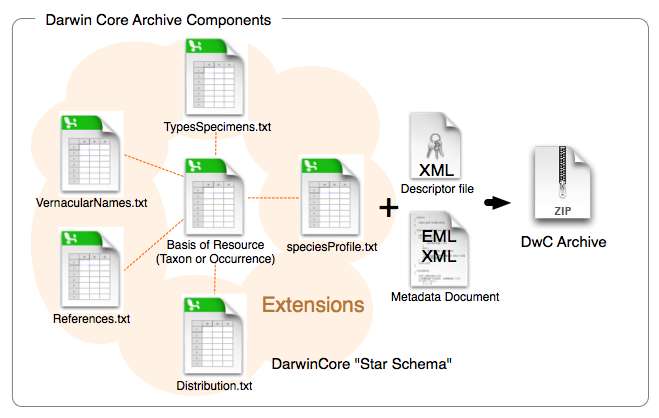
\includegraphics[width=\textwidth]{Chap5/figures/dwca.png}
    \caption{A Darwin Core Star Archive \cite{wieczorek2012}}
    \label{dwca}
    \end{figure}

Listing \ref{dwc:set} shows the comma-separated central file (Basis of Resource) containing the core details of the observation, i.e. the animal observed, and the column headings map to the descriptor file. Other linked files are typically linked by the unique ID of the observation, containing information that extends the observation and provides further context.

\noindent\begin{minipage}{\textwidth}
\lstinputlisting[caption=Darwin Core Occurrence Data, label=dwc:set]{Chap5/figures/dwc_arch/set.csv}
\end{minipage}


% Ecological Metadata Language (EML) is a metadata used by ecologists and the language is used to describe projects and those involved. This file acts as a form of certificate and descriptor as to what the data is related to and who owns it. The XML file, shown in Listing \ref{arch:dwc:eml}, outlines a sample project and users involved in the project.

% \lstinputlisting[language=XML, firstline=0, lastline=21,breaklines=true,label=arch:dwc:eml,caption=Darwin Core: EML.xml]{Chap4/listings/dwc_arch/eml.xml}

% The core file, \textit{meta.xml}, shown in Listing \ref{arch:dwc:meta} lists the files that contains the actual sensed data, as well as the terms used to describe it. Examples include: date, time, location, type of data, filename and species contained.

% \lstinputlisting[language=XML, breaklines=true,label=arch:dwc:meta,caption=Darwin Core: meta.xml]{Chap4/listings/dwc_arch/meta.xml}

% Data files contain the actual sensed data, based on how it is supported, and these files are linked in \textit{meta.xml}. For example, temperature readings or direct human sightings would be stored in a CSV file and linked, however, images or video would require the metadata to be store in a CSV file and a filepath would be referenced in the XML. The structure of the CSV file contains a header line that matches the terms in the meta file and each line would be an observation. The terms are linked to the Darwin Core glossary so the archive can be validated and processed by a DwC archive reader.

All of these files are then archived and sent as a ZIP folder throughout the network. If the sensed data is media based, then the media is included as well. Sofwtare libraries to process DwC archives are included on both DP and DA nodes.

Darwin Core is suited to K-HAS because its use in ecological observations matches our motivating scenario and the archive can be easily created by a DC node, as it does not require any heavy processing and all of the files are commonly used formats.
	
	\subsection{Middleware}
	The knowledge-processing capabilities of DA and DP nodes are the same and this is part of what makes K-HAS different from most other WSNs; both types of node run the sensor middleware, but each for different purposes. DA nodes use the middleware for administrating the network, receiving and archiving sensed data and allowing users to provide classifications. DP nodes use it for the receiving, sending and controlling the flow of processing of sensed data before it is passed on.
	
	Existing suitable middlewares have been detailed in Section \ref{sec:middleware} and our requirements for K-HAS were partially determined by the expertise of the users in our motivating scenario. Below is a list of our three core requirements:
	\begin{description}
		\item[Portability] Heterogeneous WSNs utilise nodes with different architectures and capabilities, if middleware is to be used on the nodes it must be able to run on these varied devices. 
		\item[Usability] Users of K-HAS should not be expected to have knowledge of computer science or the underlying architecture, this network should be usable by almost anyone. The same must be said for the middleware as well.
		\item[Extensibility] A closed-source middleware can be used, but it must then support all sensor nodes and data types, as well as receive regular updates. Open-source, or extensible, middleware can be used to add support for newer nodes.
	\end{description}
	
	GSN is a Java-based open-source middleware. New generic sensors can be added through XML files, while more complex sensors can be added through custom Java classes. GSN is covered in more detail in Section \ref{sec:GSN}. Because GSN can run on any architecture that supports the Java Virtual Machine (JVM), it meets our portability requirements and the web interface to provide administrative functionality makes it usable by those without any domain knowledge. Finally, the ability to add new sensors through XML means that it can be extended by almost any user of the network with very little guidance.
		
	\subsection{Knowledge Capture}\label{arch:kc}
		GSN is packaged with a web interface that allows users to see all nodes deployed and view the latest sensed data received. The web interface is targeted towards users with domain expertise and has limited functionality focussed towards sensor administration. However, it does make GSN accessible by more than one computer, as well as a variety of different architectures. For example, the admin webpage could be accessed on the machine that runs GSN, or from a tablet computer connected to the same network. We used the same approach to develop a web-based tool that provides access to all sensed data, as well as a simple interface for performing tasks, such as uploading new rules or updating the location of nodes.
		
		All sensed data is read from a MySQL database and users can view the metadata from each observation, such as location, date, time and temperature, as well as the data itself. From this, users are able to classify the data based on their role. Shown in the ontology in Chapter \ref{chap:ont}, K-HAS uses roles to control active projects and classifications; there are administrators and researchers. Researchers are involved in projects and receive notifications when relevant data has been received. They have access to the web interface and can vote on classifications for sensed data. Administrators lead projects and can create/complete them, but they also have the ability to finalise classifications. K-HAS follows a knowledge hierarchy (Figure \ref{arch:kno:hier}), with administrators at the top and DC nodes at the bottom. While there are more DC nodes in the network, their knowledge bases are more limited and classifications are trusted less than classifications made by DP nodes. Although there are fewer DP nodes, their knowledge bases are more detailed. Researchers and admins do not share a level on the knowledge hierarchy because we assume that administrators would be more experienced domain experts. For example, researchers could be students at Danau Girang, whereas an admin would be a professor with more experience. When an administrator makes a classification, all prior classifications are ignored and the feedback loop protocol is used to update nodes.

		\begin{figure}[!h]
			\centering
			\begin{tikzpicture}

			\def \h {5};
			\def \f {.7};

			\foreach \y in  {0,1,2,3} {
			    \def \w { \h*\f-\y*\f };
			    \def \v { \y*\f-\h*\f };
			    \draw (\v,\y) -- (\w,\y);
			}

			\draw (-\h*\f,0)  -- (0,\h);
			\draw (\h*\f,0)  -- (0,\h);
			\node at (0,0) [above] {DC Nodes};
			\node at (0,1) [above] {DP and DA Nodes};
			\node at (0,2) [above] {Researchers};
			\node at (0,3) [above] {Admins};
			\end{tikzpicture}
			\caption{Knowledge Hierarchy for K-HAS}
			\label{arch:kno:hier}
		\end{figure}
		
		Figure \ref{kc:loris} shows an observation where users can vote on the contents. An administrator can then confirm that classification and prevent further votes from being cast. This type of moderation means that it does not have to be specialists voting on sensed data that cannot be classified by DP nodes.
		
		\begin{figure}[h]
		\centering
		\includegraphics[width=\textwidth]{Chap4/figures/loris}
		\caption{Web Interface for Observations}
		\label{kc:loris}
		\end{figure}
		
		Viewing data for new observations is useful for gaining classifications and alerting members of a project, but viewing older sensed data allows patterns to be identified in order to create new rules. Figure \ref{kc:loris_data} shows a map of all deployed nodes in the area surrounding the field centre in our motivating scenario. When users select a node, a table is populated with all of the classified observations that it has captured; this can then be used to extract patterns from the data and create rules. For example, the three observations of the Malay civet are only seen late at night, if further observations also showed this, then we could create a rule defining the active hours of the Malay civet and, potentially, list days that it is likely to pass. These rules can then be written and uploaded to the knowledge base.
		\begin{figure}[h]
		\centering
		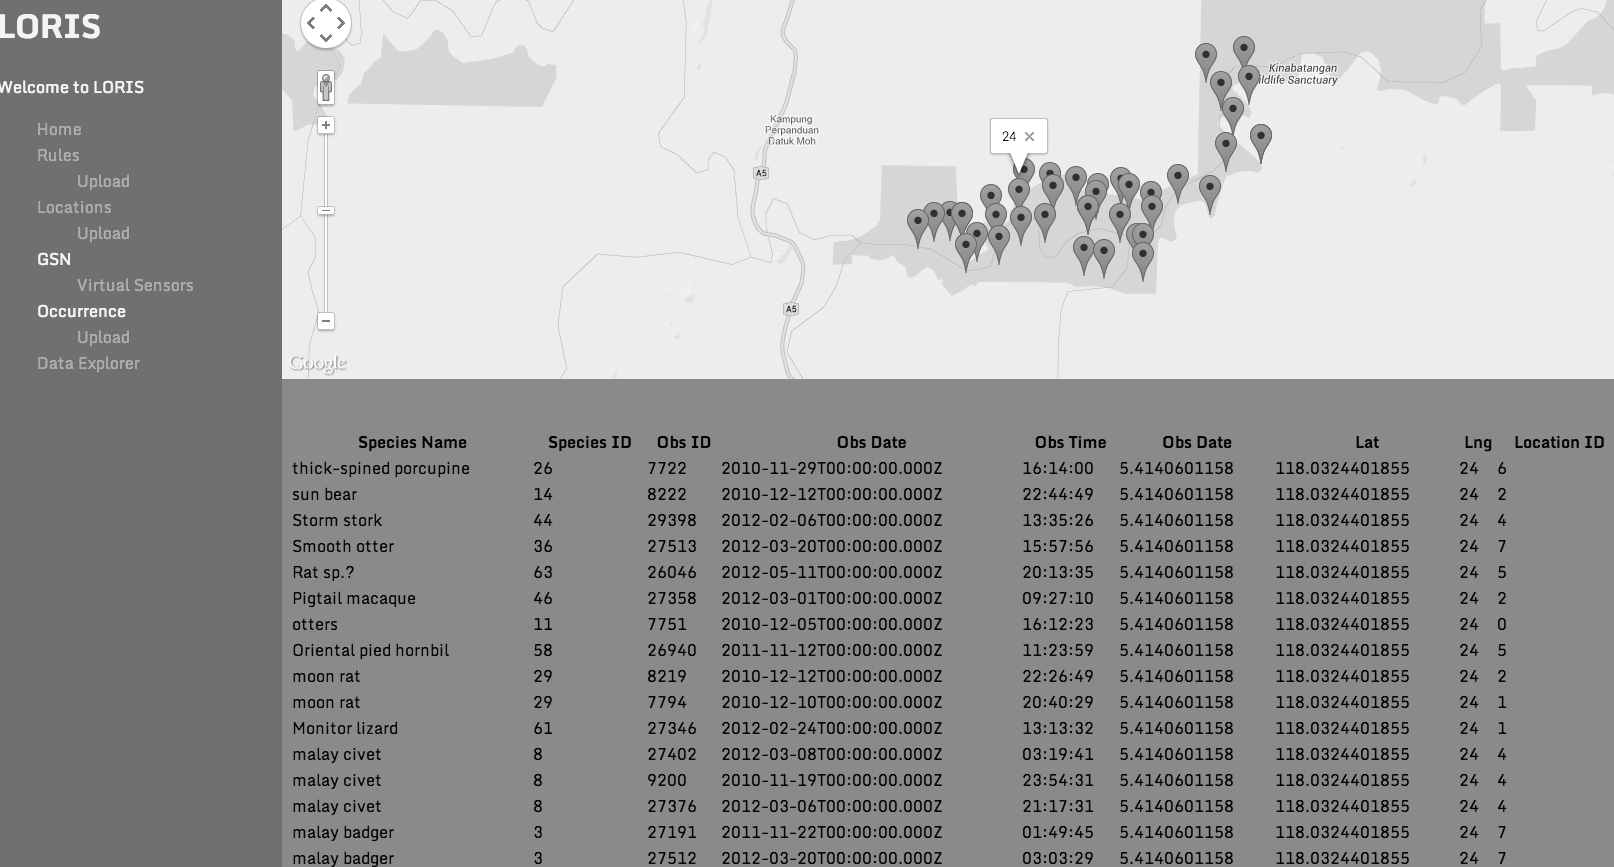
\includegraphics[width=\textwidth]{Chap4/figures/loris_data}
		\caption{Web Interface for Classified Sensed Data}
		\label{kc:loris_data}
		\end{figure}

		
	
	\subsection{Knowledge Base}\label{arch:kb}
	%Discuss drools here and the API developed for access to it from Sitesy.
	The Drools rule engine is a Java-based engine that uses forward chaining inference for the processing of rules \cite{proctor2005drools}, which means that rules are used to make meaningful inferences about data. Unlike DC nodes, which have limited knowledge processing capabilities, Drools is able to chain rules together and a rule that may not have been triggered at the start of processing may be triggered later if another inference is made. For example, a rule that is specifically for small mammals may not be triggered until an inference has been made that the image may contain small mammals based on the time and location of the observation.
	
	Drools is able to dynamically update its knowledge base, adding rules and firing them on observations that have already been loaded, as well as newer ones. This allows DP nodes to adapt to new rules and local knowledge whilst they are deployed. The use of \textit{drl} files use a mixture of Drools and Java syntax to define rules, allowing them to modify, or create, Java objects. For example, a rule could be triggered on the receipt of sensed data and create a DwC object from the received data, process it and perform checks on the result that would trigger different rules based on that result. This is one of the main reasons we chose Drools, as it can work with GSN and DwC Java objects, as well as the ability to run on any architecture that supports Java. In order to add rules to the Drools system, knowledge of the Drools syntax and, ideally, Java is required, which does make it a part of the network architecture that requires some specialist knowledge. 
	
	The functionality of Drools is extensive and the engine is very powerful, however, it does require specialist knowledge to use and manipulate rules. Using a custom developed Drools web interface , detailed in Section \ref{arch:kc}, we created a simplified interface that uses a custom REST API for Drools, allowing users to create sessions, add rules, load data and fire rules, returning the output to the interface. Users can view, and load, existing drl files, shown in Figure \ref{kc:loris_drl}. I
	
		\begin{figure}[h]
		\centering
		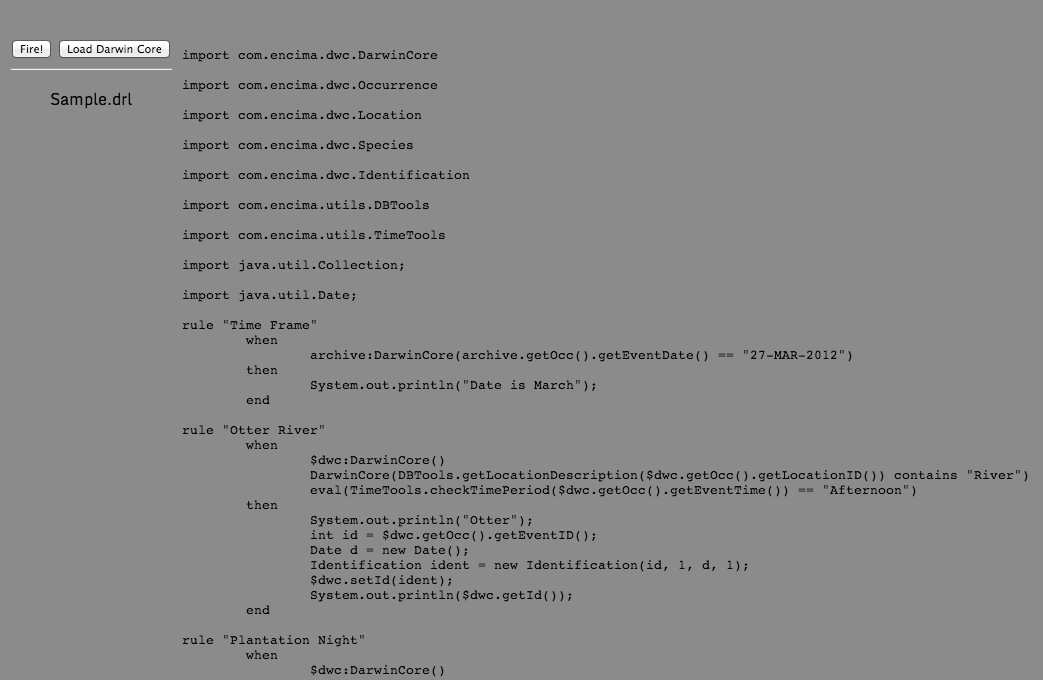
\includegraphics[width=\textwidth]{Chap4/figures/rules}
		\caption{Web Interface for Drools Operations}
		\label{kc:loris_drl}
		\end{figure}
	
	Once a file has been selected, users can view the rules and use the controls on the webpage to perform common operations. The \textit{Load Darwin Core} button loads all DwC archives that are stored in the MySQL database into the current Drools session and the \textit{Fire} button runs all loaded rules on the loaded data. If any of the rules trigger, then the output is presented to the user in the same page, allowing them to act on the results. For example, the location of observations could provide a narrowed down list of potential classifications, allowing an administrator to remove votes that do not match the list.

	Users can write new rules based on patterns gleaned from observations received during a K-HAS deployment, which can be found using the web interface and querying the database. These patterns can be encoded as rules into a \textit{drl} file and uploaded to have an immediate effect on the active knowledge base in the network. 
	
	Currently, these implementations have been developed for our motivational scenario, but much of these tools are general enough to be repurposed in order to apply to a variety of different WSNs. The Drools API can be used for any kind of sensed data and the web interface would require minor changes to be extensible.

	\subsection{Routing Protocol}\label{arch:routing}
		The routing protocol we have selected for K-HAS is not fixed for every deployment but, from our research, we modified the commonly used Mininum Cost Forwarding Algorithm (MCFA), outlined in Section \ref{bg:rp:mcfa}, as it allows for changes in the topology of the network and does not require every node to have a global view of the network.

		On deployment of all nodes, a DA node sends out a packet containing the number zero, representing the number of hops to the DA node. Nodes in range receive the packet, store it along with the identifier of the originating node and then send it once it has been incremented by one. The next nodes receive that packet and do the same until the edge of the network is reached. If a node has a number stored that is higher than the one it receives then it is replaced and sent on until the nodes at the edge of the network are reached.

		When a node wants to send data, it queries neighbouring nodes and sends to the node with the lowest hop count to the root. We modified this to run in accordance with our tiered architecture as we expect the topology to remain the same for much of the deployment.

		In MCFA, nodes do not store path information and messages are broadcast to all nodes when they are sensed.

		Firstly, our protocol runs in two modes: configuration and running. During the configuration mode, we use MCFA. Whereas MCFA does not store path information, we use the method described above to store both the hop count and the nearest neighbour. This process is carried out until all nodes of the network have a hop count (and neighbour) and a final pass is made by all nodes to find, and store, their neighbour with the lowest count. The main difference is that, unlike MCFA, not all nodes process all packets. If a packet originates from a DA node, then it is only stored by DP nodes but DP node packets are stored by both DC and DP nodes. DC nodes store it and send all data through their nearest DP node and DP nodes store other DP neighbours to delegate processing to, should a situation arise where they have too much data to process and cause a bottleneck. Configuration mode can then be run at a set interval throughout the deployment of the network, or initiated manually.

		Whilst in running mode, nodes do not query for the neighbour with the lowest hop count, or broadcast the sensed data to all nodes in range, they send to the node stored as their nearest neighbour. If that fails, then a query is sent out to find other available nodes in range and then sent to the one with the lowest hop count. If the nearest neighbour node is unavailable for more then three attempts, then it broadcasts a request to run the configuration mode again.

	
	\section{Walkthrough}\label{arch:walk}
		In this section we will explain the steps involved in the capture, and processing, of an observation when using the K-HAS architecture. Each tier is responsible for performing different actions upon the observation to ensure it is received by the DA node with an inference as to what it may contain.
		
		Not all of the features described in this section have been implemented within K-HAS and some features have only been tested on a small set of observations. For example, the image classification down to species level is a concept that we have not implemented but template matching is a commonly used practice within image processing \cite{fast1995}.

		\subsection{Scenario}\label{arch:scen}
			This walkthrough will use our motivating scenario and the type of sensed data will be images of animals in the Malaysian rainforest. In this example, we have a collection of wildlife cameras, with nodes attached to them, deployed in the forest. Projects for the rare clouded leopard and sun bear are currently active at Danau Girang. The clouded leopard is a nocturnal carnivore that uses existing paths and hill trails to travel through the rainforest and the sun bear is the smallest bear in the world and sightings are rare. It is also nocturnal and claw marks can be seen on trees that they have climbed. All of this information has been encoded onto the DP nodes and DC nodes know that images taken at night will be of a higher priority, as well as to prioritise further images at night from DC nodes that are deployed on ridges or existing trails.

			In order to explain the K-HAS architecture, we need to show the planned topology for the network in Danau Girang, which is based on the positions of the cameras in 2010. Figure \ref{topol} shows a section of the proposed topology around the field centre, with the rest of the network spreading out along the river on both sides. The triangle icon shows the location of the DA node (at the field centre), with DP nodes (square icons) placed near the DA node because of the poor range of Wi-Fi (Section \ref{tech:wifi}). Circle icons represent the DC nodes and they link to the nodes with the fewest hops to a DA node, as long as that route includes a DP node. 

			\begin{figure}[!t]
			\centering
			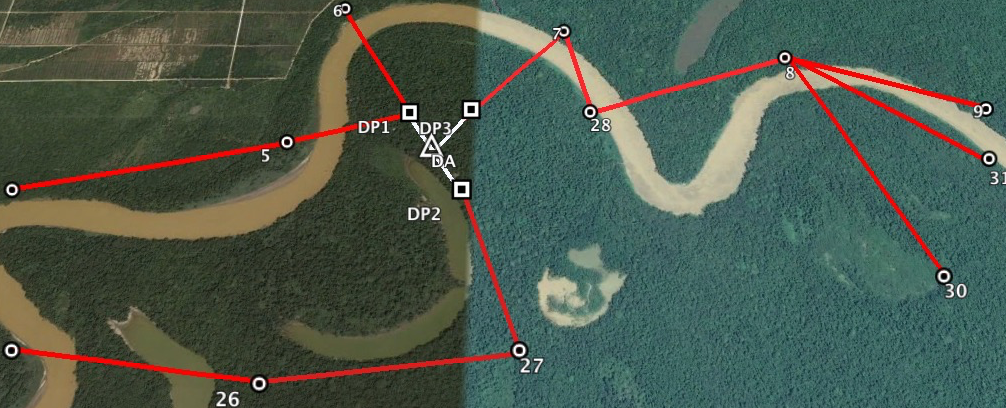
\includegraphics[width=\textwidth]{Chap4/figures/topology}
			\caption{Section of Proposed Topology for K-HAS in Danau Girang}
			\label{topol}
			\end{figure}
			
		\subsection{Data Collection}
			A DC node is deployed along a ridge in the rainforest and consists of a wildlife camera with a wireless node attached. At 0200, the infra-red sensor detects movement and the camera triggers a set of 3 images to be captured. The DC node creates the DwC archive for the observation. Terms that describe the observation, such as time, date, species identified and location, is added to the meta.xml file and links to CSV files that contain the data for each term. Any field that can be completed, such as time, location and date, is added to the set.csv file. A separate CSV file is created that holds the filename of each image that was taken. The image is shown in Figure \ref{cl2}.
			
			\begin{figure}[!t]
			\centering
			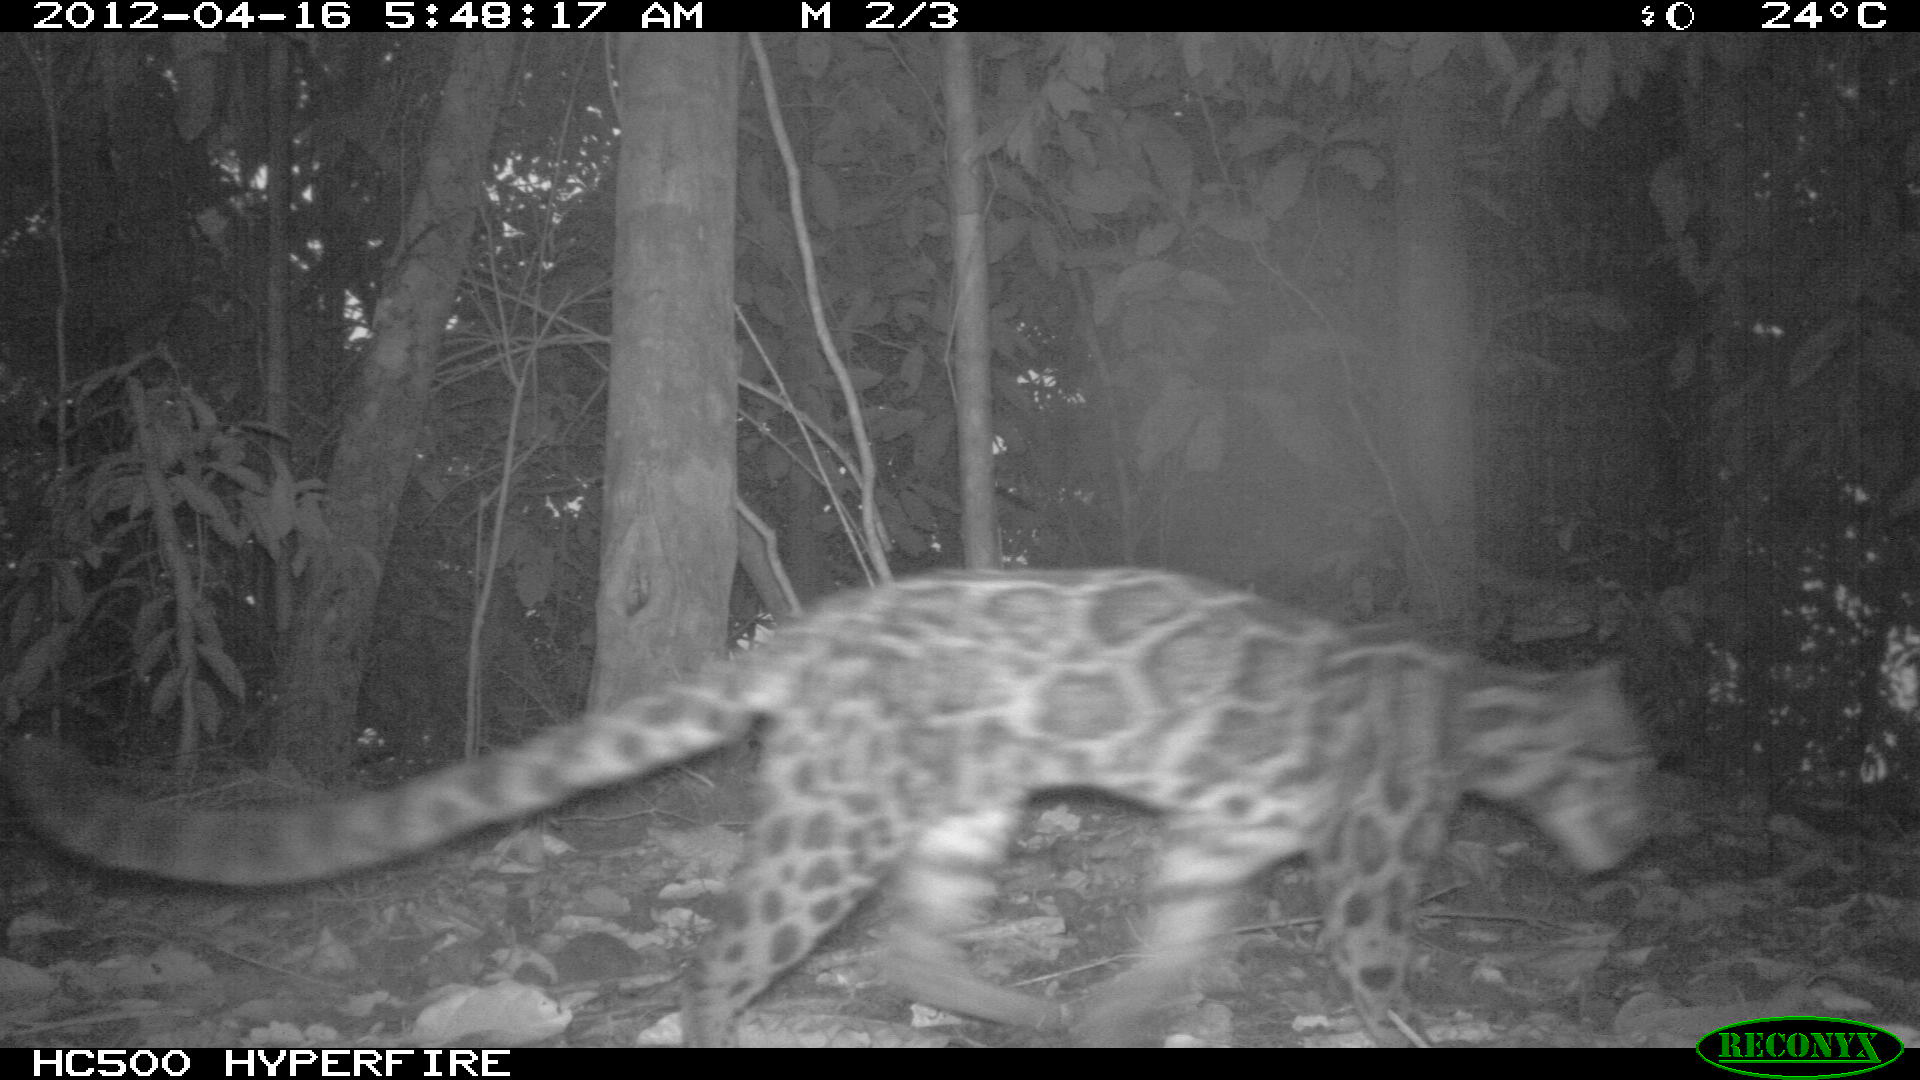
\includegraphics[width=\textwidth]{Chap4/figures/leopard2.JPG}
			\caption{Clouded leopard Image Capture}
			\label{cl2}
			\end{figure}

			\begin{figure}[!t]
			\centering
			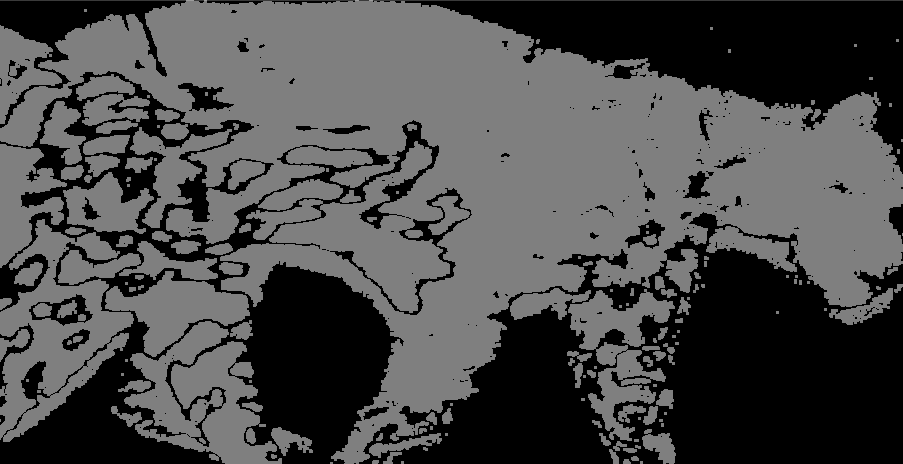
\includegraphics[width=\textwidth]{Chap4/figures/leopard_proc}
			\caption{Processed Image of clouded leopard}
			\label{clproc}
			\end{figure}
			
			The DC node runs its rules on the metadata of the images and infers that the image may contain a clouded leopard, this is because the image was taken in the early hours of the morning and the camera is deployed on a ridge. DC nodes run simple, non-chaining rules based on the file metadata and details about the node, such as location, but these rules are fixed from the time of deployment and are not updated until the network is redeployed. When bandwith is restricted, DC nodes use a queue to prioritise both their own observations and those receivied from other nodes. Observations marked as interesting are moved to the front of the queue and any others are sent afterwards.
			
			The inference is included in the archive and is compressed. The node then sends it through every DC node between the originating node and the DP node assigned. To achieve the long range communications in the forest, Digimesh is used; the low transfer rate does mean that an archive can take several minutes to send but it allows for a range of up to 1km.

	\subsection{Data Processing}			
			The DP node receives the observation and it is unzipped and processed by the Darwin Core library. If the data has been preprocessed by a DC node and marked as interesting, then the processing is prioritised, otherwise it is added to the queue. In this case, the DC node believes the observation is interesting and may contain a clouded leopard, so it would be processed before other observations that may be queued and not marked as interesting. The images are read from the filenames provided in the CSV and processed using two methods. The EXIF tags in the image are extracted and the images themselves are processed using the Open Computer Vision (OpenCV) library. A unique feature of the DP node is that it uses two radios to allow links to both DA and DC nodes. DC nodes send archives using Digimesh, to achieve long range communcation, and DA nodes use Wi-Fi, to provide a faster transfer rate than Digimesh and a more standard method that allows other devices to connect, such as mobile phones or laptops.
			
		\subsubsection{EXIF}
			EXIF (Exchangeable Image Format) tags are written to images at the time of capture. Examples of these tags can be time, date or camera serial number. The capabilities of the camera do affect how detailed the EXIF is, for example, a camera with GPS capabilities will enrich the image with the location. 
			
			Wildlife cameras have more functionality than common digital cameras, with details like moon phase, temperature and/or GPS location. Some devices even include the saturation, brightness and hue of each image. These capabilities allow the EXIF to be extremely detailed and this metadata can be used to find patterns in pictures that, when accompanied by local knowledge, assist with the classification of sensed data. 
			
			In this example, the knowledge base on the DP node is aware that clouded leopards and sun bears are nocturnal, but clouded leopards have previously only been seen when the temperature is between 30 to 35\celsius\ and only when the moon is not full. However, data on sun bear is not as complete and the knowledge base only shows that the bear is nocturnal and can be seen at any time of night in any area of the rainforest. The DP node identifies that the moon phase is not full and that the temperature is 32\celsius, from this it determines that the image could contain either animal and it cannot make a final conclusion.
			
		\subsubsection{Image Processing}
			Our Triton program, described in Section \ref{tech:sf:triton} is run on the set of three images. These images are converted to black and white and combined to build a background model for the complete set. The detected background is then removed and the final image is then searched for objects, where objects in the foreground will be shown with white pixels. The largest object is then found in the image and extracted to create a template, shown in Figure \ref{clproc}.
			
			Processed images of previously sensed images are stored on the DP node and associated with the confirmed classification, confirmed by a human or a node. Although the memory available on a DP node is typically around 32GB, this could easily fill in a matter of months if 3 full HD images were stored for every observation. Storing a single black and white template that contains a portion of the image is much more efficient and can still easily be associated with the classification made. The extracted image is then compared with the existing images, using the knowledge base to prioritise templates for comparison. In this example, nocturnal animals are prioritised and especially nocturnal animals with active projects associated. If the DP node has received an observation from the same DC node recently, then it will check for a classification on that and check for a match there first.

		As explained in Section \ref{tech:sf:triton}, species classification has not been implemented in K-HAS and templates are currently only associated with human classifications but this walkthrough describes how the process would be carried out if classification were to be implemented. These findings are written into the set.csv file of the DwC archive (Listing \ref{dwc:set}), using the identifier of the DP node as the `person' that identified the image and the scientific name for the clouded leopard as the species identified in the image. The archive is then zipped and sent on to the DA node, sending observations of interest first and delaying observations that have been found to contain nothing of interest.
				
		This observation is the first trigger from the DC node in the past few hours, so there are no recent classifications. However, processing of the metadata showed that the image was taken at night, so the DP node would use its knowledge base to match the images to templates of nocturnal animals first. Triton could then find a match to an existing template of a clouded leopard and completes its classification.
	
		\subsubsection{Classification}
		The metadata processing of the image shows that it could be any nocturnal animal that is known to come out when the moon is not full and the temperature is 32\celsius. This is not a complete classification but the image processing has found a match. 		
	\subsection{Data Aggregation}		
			Upon receiving a DwC archive, it is unarchived and processed by Darwin Core libraries, called by the middleware running on the node. The resulting archive is then inserted into a MySQL database and the files themselves are stored in a directory that maps to the DC node that captured the original observation. At the field centre, three users of the system have subscribed to updates for observations of clouded leopards.
			
			As the archive is processed by the library, the species is extracted and this triggers a rule to notify the subscribers. The rule then queries the database and finds their preferred method of communication. In this case, one is a lecturer and wants to be emailed while the two remaining are students and want to be notified via Twitter. An email is generated that contains the time, location and content of the observation, with the images attached, and sent on to the lecturer. The students are sent a short tweet that tells them a clouded leopard has been spotted and a link to the middle image in the sequence is provided; the middle image is used because local knowledge has shown that it is the most likely to contain the full subject in the image. In order to maintain privacy, a `direct message' can be sent on Twitter so this message is not public.
			
			The middleware on the node supports a web interface to allow users to perform administrative functions on the network, such as deploy a new node, on top of this there is a custom made website that shows all observations for every DC node. This allows users to log on and classify the images. In this case, the lecturer receives the email notification, reviews the attached images and clicks on the link to access the website to inform the DP node that the classification was correct. Due to the administrator position the lecturer has on the system, he is able to stop any users voting on the image and to simply confirm the classification.
			
			When a user classifies the observation, they see that a clouded leopard has been spotted in the same area on the same day for the past 5 weeks and they create a rule to automatically classify images from this camera that have a similar time (within an hour) and have an object extracted from them by the image processing. The user can then upload the rules through the same web interface and it will instantly become active on the system.

			If there was no classification, then users would be able to vote on the contents and use the classification with the highest vote, or the classification made by an administrator. Once a classification has been made, it is stored in the database and written to the archive. This triggers the DA node to send that classification on to the DP node that sent the original archive. In this case, the DA node informed the DP node that it has been confirmed as a clouded leopard and the DP node then stores the extracted image in the directory of clouded leopard templates, to assist with future classifications. This updated template causes the rule base of the DP node to be updated so similar data processed in the future would be correctly identified. The longer the network is deployed, the more knowledge DP nodes gain and the more accurate their classifications can be. For example, a change in season could cause a new, previously unknown animal to migrate to the rainforest. With human assistance, the animal can be identified and determined whether it is of interest. This knowledge can then be stored and sent on to DP nodes to prioritise and classify correctly the next time that it is captured. The feedback loop protocol is currently only a design and has been minimally implemented as a proof of concept.
					
	\section{Conclusion}\label{arch:conc}
		In this chapter we have explained the architecture we have developed to allow knowledge to be encoded and utilised within a wireless sensor network. Using tiers of nodes, with varying levels of knowledge-processing capabilities, we can process observations within the network and deliver data that has, where possible, already been classified. Working as more of a subscribe-push method, users do not have to check a DA node for new data, instead it is sent to them if it has been found to be part of a project they are subscribed to. If not, then the data is accessible to all users of the network through a web interface.

		%COMPARE WITH OGC SWE HERE!
		%http://essay.utwente.nl/59473/1/scriptie_R_de_Lange.pdf
		Using GSN as the application middleware allows sensors to be added, modified and maintained by those without technical knowledge and ensure future interoperability. However, it is not a standardised approach and using an architecture that implements the standard OGC SWE\cite{botts} would allow for interoperability through the use of standards not just for sensor networks but the Web as well. 
		
		One of the key features of K-HAS is that it is not a static deployment. The knowledge that the network holds at the time of deployment will rarely be the same as the knowledge held after a few months. Humans enrich the existing knowledge base and the nodes are able to make inferences about the data they are sensing, improving their classifications the longer they are deployed. When developing this architecture, GSN was the most robust architecture of those that we researched and tested, the support for many databases, administrative interface, native support for many widely used sensors meant that it was a better choice than a middleware that adopted the OGC SWE standards, especially as we were not interacting with SWE systems in our motivating scenario. However, while GSN is stable and mature, its large codebase does mean that there are dated features, such as using SOAP instead of REST and an unintuitive web interface that does not utilise web sockets. A middleware with similar automotation on receipt of sensor data could be used instead of GSN that did follow the standards set out by the OGC. We believe that this should require few changes to the core K-HAS architecture as it currently stands.
		
		In Chapter 6, we explain how we implemented a variation of K-HAS in our motivating scenario and Chapter 7 shows our evaluation of the K-HAS architecture, but Chapter 5 will first outline the development of an ontology to support the architecture described here.
		
			
			
			
			
			
			
			
			

\chapter{An Ontology for the K-HAS Architecture}\label{chap:on}
In this chapter, we explain the ontology that we developed to formally the components within K-HAS, the structure of the sensed data and the users involved with the network, as well as the format of the sensed data that is passed through the network.

This ontology provides those wanting to use K-HAS with a representation that is easy to reuse and deploy in a number of different scenarios, or even to select parts of the ontology that meet their requirements and implement those. 
\section{Background}\label{bg}

%COMPLETE THE BACKGROUND FOR EXISTING ONTOLOGIES

%MAYBE INCLUDE SUBSECTION FOR DEVELOPMENT METHODOLOGIES (IS THIS 2 DIFFERENT PAPERS?)

K-HAS was developed in order to provide a generic architecture for wireless sensor networks to utilise the local knowledge contained within their environment to process sensed data and, therefore, make more efficient use of the network bandwidth by prioritising sensed data that is deemed to be more valuable. We have defined local knowledge as knowledge of an area that has been gained through experience, or experimentation.

Before we were able to implement K-HAS, we needed to model the flow of knowledge within the network. Developing an ontology for K-HAS means that we can do this, as well as provide a computer-readable model for all of the classes and components used by K-HAS, and the relationships between them.

Making it computer readable has allowed us to reuse classes in the development of software for each tier. For example, we were able to develop a common Darwin Core java library that is used in this ontology and in our GSN middleware to unzip and process received archives.

During the development of the K-HAS ontology, we researched existing ontologies that were commonly used in the domains that K-HAS covered. These included scientific observations and sensor hardware.

Looking into existing ontologies, we found that there had been many surveys on representing sensors in the semantic web: \cite{Compton2009}, \cite{Janowicz2010}, outlines the existing work. These surveys clearly highlighted that these ontologies had been split into two branches; observation-centric and sensor-centric.

Observation-centric ontologies focus on the data that is sensed, and its content; whereas sensor-centric ontologies detail the components that make up a sensor, and the operations they perform to turn sensed data into an output.

We found no ontologies that linked these concepts together to show the flow of data within the network and the role that each sensor plays in delivering this data. This could be because other WSNs do not integrate structure, hardware and sensed data in the same way as K-HAS or due to the fact that most WSNs do not process their sensed data until they reach a base station, so they would not need to model their data structure within the network. Because of this, we developed an aligning ontology that reuses existing ontologies, where possible, and introduces new classes that allows these ontologies to interlink. The result is an ontology that covers the flow of sensed data from the point of capture to the point it is received, processed, reviewed and stored at the end point of the network. Not only does the ontology cover how the data changes as it flows through the network but also the roles and capabilities of each tier.

K-HAS has been developed to be used with any sensors and is not specific to wildlife cameras, therefore we also looked into sensor-based ontologies that concentrate on the hardware and the individual capabilities of each device within the network.

From this we have categorised relevant existing ontologies into Observation-Centric and Sensor-Centric ontologies.

\subsection{Observation-Centric Ontologies}
%This can be seen as an ontological representation of the OpenGIS Observations and Measurements (O\&M) Standard \cite{botts2008ogc} that provides a framework for representing observations, measurements and procedures within sensor systems.

\subsubsection{OBOE}\label{OBOE}
The Extensible Observation Ontology (known in reverse as OBOE) is a popular suite of ontologies used to represent scientific observations \cite{Madin2007b}. Initially starting as base ontology for ecological observations, it has now grown into a suite of extensions that make it suited for chemistry, bioinformatics, anatomy and others. OBOE is represented by OWL-DL \cite{McGuinness2004} and allows the characteristics of a generic scientific observation to be linked to domain specific characteristics.

OBOE focuses on the concept of an \textit{observation}, which is made up of an entity, a measurement and a characteristic \cite{Madin2007}. An example of an observation could be a researcher observing an animal (the entity) and recording the gender (the measurement) as male (the characteristic). A single observation could then consist of multiple observations within it, such as gender, location, species and the number of species observed. 

    \begin{figure}
    \centering
        \scalebox{0.73}{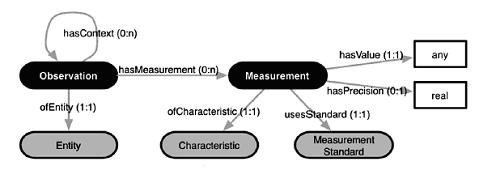
\includegraphics{Chap5/figures/OBOEcore.JPG}}
    \caption{The Core of an OBOE Observation}
    \label{oboe}
    \end{figure}

Figure \ref{oboe} shows the basic structure of a core OBOE observation, outlining the five key classes that are linked by seven properties. While this is the core structure of OBOE, domain specific extensions have been implemented by utilising `extension points' that are part of OBOE's core. OBOE follows the O\&M Standard (below) very closely, providing extensions to the core classes that allows more information about each to be encoded, adding context and enhancing the value of an observation.

The primary benefits of OBOE are that it is generic enough to cover almost all types of scientification observation and domain extensions allow for more specific details to be stored.

\subsubsection{O\&M}
The OpenGIS Consortium (OGC) Observations and Measurements Standard aims to provide a framework suitable for recording any observation made by a sensor, regardless of the domain \cite{Botts}. 

The key difference, when compared to other ontologies, to note with O\&M is that \textit{observation} and \textit{measurement} are not just classes. They also denote an action.
An observation is an action that causes a result, yielding a value and a measurement is a set of operations that provide some result(s).

O\&M provides a conceptual model, as well as XML encoding for observations and measurements. The listing \ref{omxml} shows an observation of a vehicle in a given time and place. Similar to the encoding of a measurement with the standard and protocol used in OBOE, O\&M provides support for the recording of the procedure used to gain the measurement for the observation. 

\begin{lstlisting}[caption=An Observation of a Vehicle encoded in O\&M, label=omxml, breaklines=true, language=XML]
 <?xml version="1.0" encoding="windows-1250"?>
 <om:GeometryObservation gml:id="geom1610" 
 xmlns:om="http://www.opengis.net/om/1.0" 
 xmlns:xsi="http://www.w3.org/2001/XMLSchema-instance" 
 xmlns:xlink="http://www.w3.org/1999/xlink" 
 xmlns:gml="http://www.opengis.net/gml" 
 xsi:schemaLocation="..Specialization_override.xsd">
   <om:samplingTime>
     <gml:TimeInstant>
       <gml:timePosition>2009-09-16T17:22:25.00</gml:timePosition>
     </gml:TimeInstant>
   </om:samplingTime>
   <om:procedure xlink:href="urn:ogc:object:procedure:ifgi:GPS"/>
   <om:observedProperty xlink:href="urn:ogc:def:phenomenon:OGC:Shape"/>
   <om:featureOfInterest xlink:href="urn:ogc:object:feature:vehicle"/>
   <om:result>
     <gml:Point srsName="urn:ogc:crs:epsg:4326">
       <gml:pos>40.7833 -73.9667</gml:pos>
     </gml:Point>
   </om:result>
 </om:GeometryObservation>
 \end{lstlisting}
 
 The listing shows that an observation centres around a \textit{feature of interest} that can be a physical object and the measurement is the detection of the vehicle at the recorded location. Figure \ref{oandm} shows a basic diagram of the ontology. While the event of a feature is linked, it is clear that the main focus is on the observation and the measurement associated with it.

    \begin{figure}[h]
    \centering
	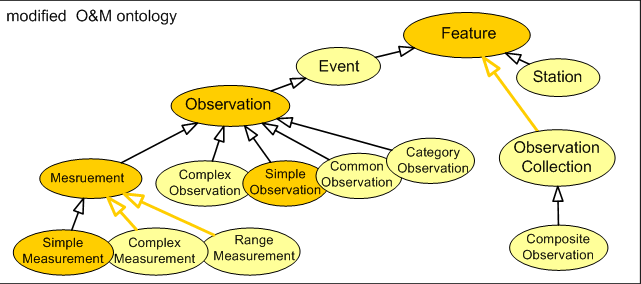
\includegraphics[scale=0.65]{Chap5/figures/o&m_ontology.png}
    \caption{The OGC O\&M Ontology}
    \label{oandm}
    \end{figure}
 
The structure of an observation within O\&M is focussed on the action and the result, this makes it suited for sensor networks across many domains that perform a wide range of observations. Because the users of the O\&M standard are spread across many domains, each with their own terms and definitions, the creation of an ontology for the standard aimed to remain as generic as other observation-centric ontologies. 

\subsubsection{Darwin Core SW}\label{bg:dwc}
Darwin Core is a body of standards for representing, sharing and storing observations, we explain this in more detail in Section \ref{arch:tech:dwc}. While it does not have the extensions available to OBOE, Darwin Core is extremely concise for recording observations within the biological diversity domain and aims to be a standard reference for sharing these observations.

The standard structure of a Darwin Core Archive (DwC-A) is a star record; an archive of files with a core metadata file that describes the content of all other files within the archive.

The record shown in figure \ref{dwca} represents a DwC-A that conforms to the star schema. The ecological metadata language document contains all of the details about the project, such as who is involved, the institution code, contact details and the project(s) related to the observation, shown in Listing \ref{dwc:eml}.

\lstinputlisting[language=XML, caption=Darwin Core Ecological Metadata File, label=dwc:eml]{Chap5/figures/dwc_arch/eml.xml}

The descriptor file is an xml document that contains the column headers in the attached files and the mappings of those headers to DwC terms, an example file is shown in Listing \ref{dwc:meta}. This file shows that this is an archive containing the sighting of an individual, and that the sighting has been split into two files. The largest benefit of Darwin Core is its modularity. Extension files can be added to enrich the data for each occurrence. In this example the extension file is named as \textit{images.csv} and contains image-based evidence to support the observation.

\noindent\begin{minipage}{\textwidth}
\lstinputlisting[language=XML, caption=Darwin Core Descriptor File, label=dwc:meta]{Chap5/figures/dwc_arch/meta.xml}
\end{minipage}

    \begin{figure}
    \centering
      \scalebox{0.53}{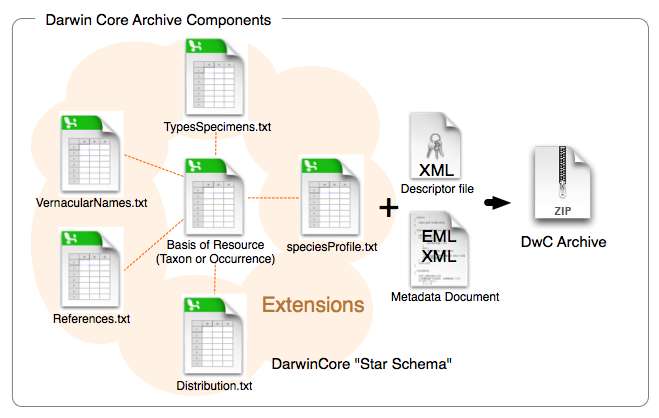
\includegraphics{Chap5/figures/dwca.png}}
    \caption{A Darwin Core Star Archive}
    \label{dwca}
    \end{figure}

Listing \ref{dwc:set} shows the comma-separated central file (Basis of Resource) containing the core details of the observation, i.e. the animal observed, and the column headings map to the descriptor file. Other linked files are typically linked by the unique ID of the observation, containing information that extends the observation and provides further context.

\noindent\begin{minipage}{\textwidth}
\lstinputlisting[caption=Darwin Core Occurrence Data, label=dwc:set]{Chap5/figures/dwc_arch/set.csv}
\end{minipage}

In order to represent DwC occurrences in an ontological format, work has been done to represent Darwin Core terms, as an ontology, in OWL. Darwin-Semantic Web (Darwin-SW) \cite{dwc_sw} is the project that aims to do this and many of the core terms associated with an occurrence have already been formalised.

    \begin{figure}[h]
    \centering
        \scalebox{0.23}{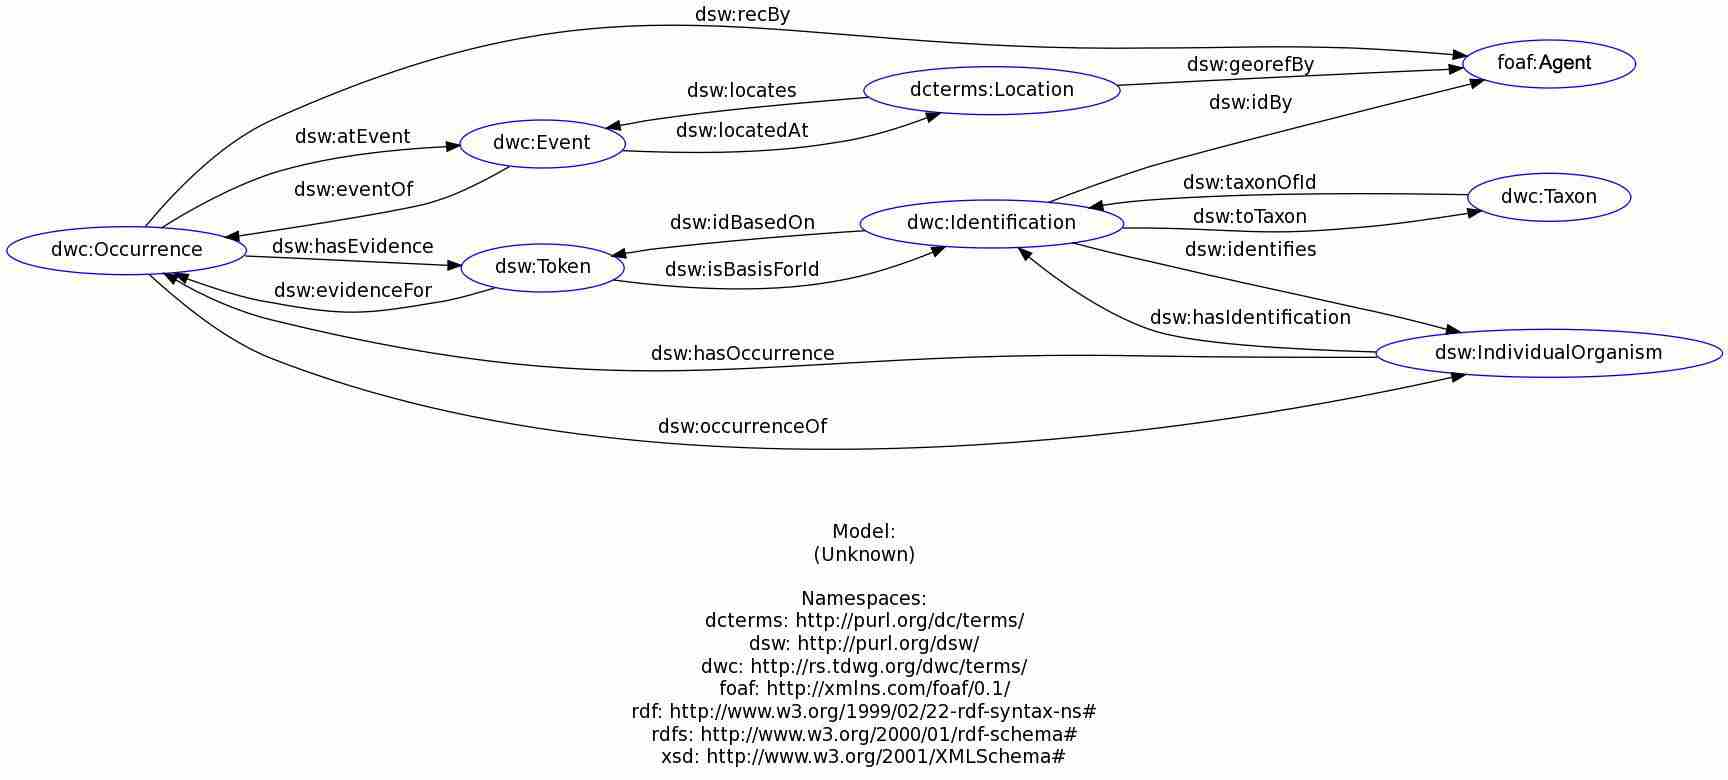
\includegraphics{Chap5/figures/dsw.jpg}}
    \caption{Darwin-SW}
    \label{darwin-sw}
    \end{figure}

While Darwin-SW does not represent all of the classes within the DwC namespace, it contains the core classes required to record an occurrence, to a more-detailed level than OBOE. The downside of this is that the specificity of the terms limits DwC to ecological observations, making it far less generic than OBOE and other alternatives. There are positive aspects that, for those that need to record ecological observations, DwC allows for a greater level of detail and  can be mapped to OBOE with ease.

\subsection{Sensor-Centric Ontologies}
Sensor-centric ontologies are more focussed on the structure of the sensor, the network and the sensing processes involved. 

\subsubsection{SensorML}
The Sensor Markup Language (SensorML) Standard has been developed by the OGC, and complements the O\&M Standard, to enable the discovery and tasking of internet-connected sensors \cite{Botts}.

SensorML provides an XML schema for describing a sensor, its capabilities and the processes available. At the core, SensorML comprises of:
\begin{enumerate}
  \item Component - A physical process that transforms information from one form to another.
  \item System - Model of a group of components.
  \item Process Model - Atomic processing block used within a Process Chain.
  \item Process Chain - Composite block of Process Models.
  \item Process Method - Definition of the behaviour of a Process Model.
  \item Detector - Atomic part of a Measurement System.
  \item System - Array of components, relates a Process Chain to the real world.
  \item Measurement System - Specific type of System, mainly consisting of sampling devices and detectors.
  \item Sensor - Specific type of System that represents a complete Sensor.
\end{enumerate}

These definitions outline the core concepts of SensorML, a \textit{system} that performs one (or more) process(es) and is comprised of a group of \textit{components} \cite{Robin2006}. A SensorML document allow for a general, formal specification of a \textit{sensor} and its capabilities. The document describes a \textit{component}, outlining what data it reads in and the output once it has been processed. Several of these \textit{components} can the be used to create a \textit{system} and the primary goal of SensorML is to describe the process of how an observation came to be, focussing on the technical featuresof the node.

%\begin{lstlisting}[caption=SensorML Sample Document, label=sensormldoc, breaklines=true]
%<Component>
%  <keywords>
%    <KeywordList>
%      <keyword>weather station</keyword>
%  ...
%    </KeywordList>
%  </keywords>
%  <identification>
%    <IdentifierList>
%      <identifier name="uniqueID">
%        <Term definition="urn:ogc:def:identifier:OGC:uniqueID">
%          <value>urn:ogc:object:feature:Sensor:IFGI:thermometer123</value>
%        </Term>
%      </identifier>
%  ...
%      </identifier>
%    </IdentifierList>
%  </identification>
%  <classification>
%    <ClassifierList>
%      <classifier name="sensorType">
%        <Term definition="urn:ogc:def:classifier:OGC:1.0:sensorType">
%          <value>thermometer</value>
%        </Term>
%      </classifier>
%    </ClassifierList>
%  </classification>
%  <capabilities>
%    <swe:DataRecord definition="urn:ogc:def:property:capabilities">
%      <swe:field name="status">
%        <swe:Text definition="urn:ogc:def:property:OGC:1.0:status">
%          <gml:description>System operating values.</gml:description>
%          <swe:value>active</swe:value>
%        </swe:Text>
%      </swe:field>
%    </swe:DataRecord> 
%  </capabilities>
%  <inputs>
%    <InputList>
%      <input name="atmosphericTemperature">
%        <swe:ObservableProperty definition="urn:temperature"/>
%      </input>
%    </InputList>
%  </inputs>
%  <outputs>
%    <OutputList>
%      <output name="temperature">
%        <swe:Quantity definition="urn:ogc:def:property:OGC:1.0:temperature">
%          <gml:groupName codeSpace="ObservationOffering"> Weather </gml:groupName>
%          <swe:uom code="Cel"/>
%        </swe:Quantity>
%      </output>
%    </OutputList>
%  </outputs>
%</Component>
%  \end{lstlisting}

\subsubsection{SSN}
The Semantic Sensor Network (SSN) Ontology is the most fitting ontology for our requirements, as it covers systems processes and observations. Developed by the W3C after an extensive review of existing ontologies \cite{lefort2011semantic}, the SSN ontology is designed to allow focus on a variety of perspectives, such as the sensor within the network or the data that has been observed.

    \begin{figure*}
    \centering
        \scalebox{0.50}{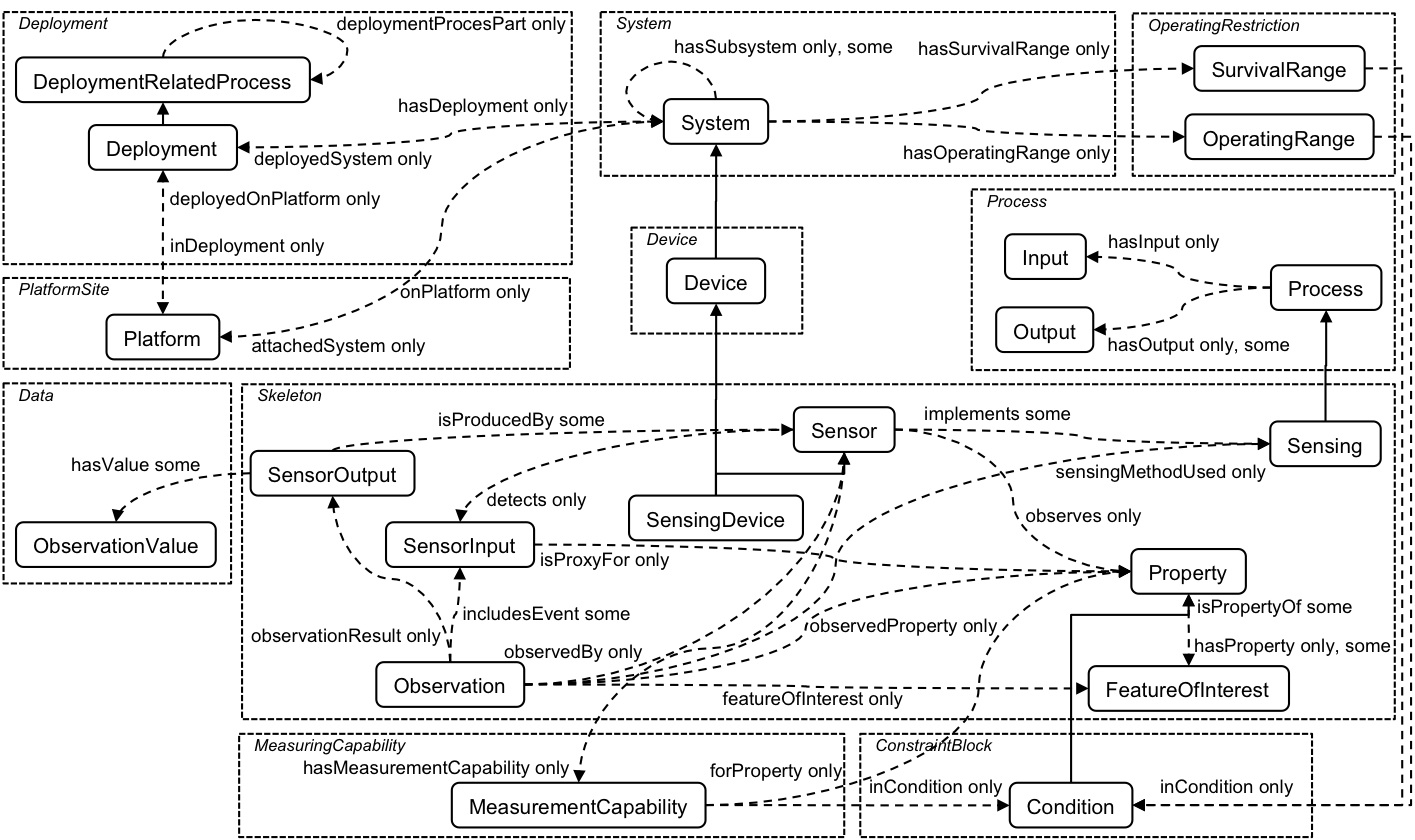
\includegraphics{Chap5/figures/ssnont.jpg}}
    \caption{SSN Ontology}
    \label{ssnont}
    \end{figure*}
    
Figure \ref{ssnont} shows the model for the SSN ontology, displaying the relationships that connect each class, as well as their associated properties. It also highlights the modular approach that has been taken, separating the system from the process and the observation.

The observation pattern of SSN is centred around `Stimuli-Sensor-Observation', which can be simply described by an event causing a sensor to trigger and create an encompassing observation to store details about the event, as well as the device that recorded the event. While SSN is focussed on sensors, capturing the measurement capabilities of each sensing device that makes up a system and specifics on its lifespan, the development of the ontology arose from the review of sensor-centric ontologies as well, recording data about observations is a structure very similar to O\&M.

\subsubsection{Findings}
There are many ontologies that are suited for sensor-based scientific observations and ontologies that allow for the description of sensor hardware are very complete. However, in our research, we were unable to find a complete ontology that allowed for a sensor to be described as well as specifics of the observation. SSN was the closest that we found for this, but it was still very hardware focussed and aimed at a technical audience. SSN primarily describes the hardware of each node and their capabilities, whereas our requirements are for both hardware and sensed data to be represented in a single ontology.

We found that many of these ontologies satisfied many subsections of K-HAS completely, meaning that it would be unnecessary to reproduce these concepts. From these findings we have developed an alignment ontology that connects ontologies across multiple domains to support our proposal of K-HAS, creating an ontology that is both sensor-centric and observation-centric.

\section{Method}
% *Outline standard ontology development method
% *Explain our variation
% Reference the various methods outlined

Before we began development, we researched existing methods that have been used to develop current ontologies. From this, we found three well-documented methodologies; the methodology used to develop the Toronto Virtual Enterprise (TOVE) ontolgy, the Methontology and the methodology used to develop the Enterprise Model ontology.

The methodology by Uschold and King \cite{Uschold1995}, used to develop the Enterprise ontology, is a four step method that was most suited to the processes we expected to follow. The steps are not covered in great detail in the original paper but, research since provides greater detail for each step.

\subsection{Identify Purpose}
The aim of this step is to identify why the ontology is being built and what requirements it is supposed to fulfil. This includes considerations, such as the audience, the intended purpose and the specificity of the ontology.

Other methodologies have used more structured methods to informally identify the requirements of the ontology. Gruninger and Fox \cite{Gruninger1995} propose competency questions; these are questions that are used to identify the problems that the developed ontology is developed to solve. These questions can act as a benchmark, showing that an ontology is sufficient if it can solve the questions raised here.

\subsection{Build the Ontology}
Building the ontology can be broken down further into 3 smaller steps: capture, code and integrate existing ontologies.

\subsubsection{Capture}
 % - identify key concepts, provide unambiguous text definitions
The capture stage involves defining the concepts and terms that the ontology will model, as well as how they map to the real world. This can be done in one of three ways:
\begin{enumerate}
\item Top Down - Starting with the core conepts, create the more specialised classes until you have identified all subclasses.
\item Bottom Up - This process begins with the more specialised classes and grouping them into the more general classes towards the top of the heirarchy.
\item Middle Out - A combination of the two, this process involves specialising, and generalising, the classes identified in the middle layer of the hierarchy.
\end{enumerate}
% REFERENCE THE ONTOLOGY 101 PAPER
As for the capture of the knowledge used to identify the classes needed, this is an area that has been documented, but primarily provides recommendations. \cite{Fernandez-Lopez1999} suggests interviews with domain experts, iteratively brainstorming with a group actively involved in the development of the ontology. This stagehas often been referred to as the knowledge-acquisition stage.
% and **REFERENCE** recommends the use of Common KADS \cite{Hoog1992}, a knowledge analysis methodology used to develop knowledge-intensive systems.

\subsubsection{Code}
 % - perform the above step in a formal language (i.e. OWL)
This step involves coding the terms identified in the previous step into a formal language, such as the Web Ontology Language (OWL).

\subsubsection{Integrate Existing Ontologies}
 % - join all ontologies that match/overlap with the identified terms
Some of the literature (REFERENCE) recommends that this step is carried out at the same time as the two steps prior, so that the ontology is developed with existing ontologies in mind. This also allows overlap to be identified, and incorporated, early. Being aware of commonly-used ontologies within the domain, before development begins, is a more logical approach and does avoid the need to create new terms for existing concepts.

Existing ontologies can be integrated by importing them and linking the existing terms to the terms identified in the ontology that is being developed. However, there is also the method of developing the ontology completely, so that it is consistent without the need to rely on existing ontologies and creating `sameAs' relationships between the terms identified and only the required terms in the existing ontologies.

In \cite{Jimenez-Ruiz2008}, it is recommended that, when importing external ontologies, the whole ontology is not used. Rather, one should aim to extract only the required fragments from the external ontology that are relevant to the concepts in the developed ontology.


\subsection{Evaluation}\label{method:eval}
For the evaluation, Uschold and King adopt the definition of \cite{Fernandez-Lopez1997}: “to make a technical judgement of the ontologies, their associated software environment, and documentation with respect to a frame of reference..." The frame of reference may be requirements specifications, competency questions, and/or the real world”.

There are some well documented methods for evaluating ontologies in the literature, \cite{Uschold} proposes using the competency questions, used in the first step, to ensure that they can all be fully answered by the finished ontology. 

\subsection{Documentation}
Although this step is listed at the end of the development cycle, it seems more fitting to document all major aspects of the ontology as it is being developed. Documentation of the ontology should include: any assumptions, all concepts introduced, all ontologies that have been incorporated (by whatever means) and any primitives used for the definitions of concepts.

\section{Results}
This section details our results when using the Uschold and King methodology, accompanied by more recent research for particular steps, to develop the K-HAS ontology. 

\subsection{Identify Purpose}\label{ident}
The need to create the K-HAS ontology was partly due to the reasons outlined by Gruninger and Fox \cite{Gruninger1995}, we had identified a problem as we were developing a sensing architecture that utilised local knowledge: how could we formally represent the flow of knowledge and sensed data throughout a wireless sensor network?

To determine the scope that K-HAS should cover, we identified a set of competency questions that represent what we expect K-HAS to cover within the domain. In order to present this, we used an approach similar to that of \cite{Choi2010}, which can be seen in Table \ref{tab:comp_qs}.

\begin{table}[h]
\caption{Competency Questions} 
\begin{tabular}{ p{10cm}}
\hline
\textbf{Competency Questions}\\ 
\hline
Find all \textbf{Occurrences} of an \textbf{Individual} \\
Find all \textbf{Occurrences} of an \textbf{Individual} at a \textbf{Location}\\
Find all \textbf{Occurrence} within a specified \textbf{Date} and \textbf{Time} range \\
Find all \textbf{Sensors} that have recorded an \textbf{Occurrence} of an \textbf{Individual}\\ 
Find all \textbf{Locations} of an \textbf{Individual}  \\
Find the storage location of a \textbf{Project} \\ 
Find all \textbf{Projects} containing an \textbf{Individual}\\
Find all \textbf{People} involved in a \textbf{Project}  \\
Find all the \textbf{Evidence} that supports an \textbf{Occurrence}\\
Find all the \textbf{Types} of evidence that supports an \textbf{Occurrence} \\
\hline 
\end{tabular}
\label{tab:comp_qs}
\end{table} 

These questions allow us to identify the core concepts that the ontology needs to represent, as well as serving as a tool to evaluate the completed ontology.

\subsection{Build the Ontology - Capture}\label{buildcapture}
This part of the development cycle is the identification of the concepts and their implementation. The first step is capture the knowledge that will be used to identify the core concepts within the ontology. 

To capture the knowledge for the ontology, we used a combinatorial approach of those outlined in the literature. We interviewed domain experts, as well as overseeing a basic implementation of a system, and we iteratively brainstormed the concepts throughout the development cycle.

Over the course of eighteen months, which involved 2 field visits and several brainstorming meetings, we identified the core concepts that the ontology would need to contain, as well as the properties that would link them. From this, it would seem that we followed the \textit{Top-Down} approach, but the first visit with domain experts also allowed us to identify some of the more specialist classes early on in the development cycle. Thus, it seems that in practice we followed a more \textit{Middle-Out} approach.

Table \ref{tab:concepts} outlines the core concepts we have identified for K-HAS to be complete, as well as the definitions we have used for the architecture. When integrating existing ontologies, the definitions of similar terms would need to match with our definitions or we would not deem them the same as the K-HAS concepts.

\begin{table}
\caption{K-HAS Concepts} 
\begin{tabular}{p{5cm}|p{2cm}|p{5cm}}
\hline
\textbf{Concept} & \textbf{Subclass Of} & \textbf{Definition}\\ 
\hline
Occurrence & - &  \\
Identification & - &  A text-based recording of the content of an Occurrence\\
Evidence & - & Media to support the Identification, such as a photo or recording.\\
Location & - & The location of the Occurrence.\\ 
Date & - & The date of the Occurrence.\\
Time & - & The time of the Occurrence.\\ 
Project & - & Project(s) that can contain many Occurrences\\ 
Node & - & A device with sensing capabilities.\\ 
Data Collection (DC) Node & Node & Node with limited knowledge-processing capabilities charged with sensing a feature (or features) of its environment. \\
Data Processing (DP) Node & Node & Node with knowledge-processing capabilities charged with serving a subset of DC Nodes and processing their sensed data. \\
Data Aggregation (DA) Node & Node & Node with knowledge-processing capabilities that stores all knowledge and sensed data for the whole network. \\
Person & - &\\ 
Administrator & Person & Person in charge of a project (or projects). \\
Worker & Person & Person involved with a project. \\
\hline 
\end{tabular}
\label{tab:concepts}
\end{table}

Mapping these concepts, a diagram of the base K-HAS ontology is shown in Figure \ref{khas_base_ont}. The next step is to create the ontology and map the concepts identified to existing ontologies within the same domain space(s).

    \begin{figure}[h]
    \centering
        \scalebox{0.17}{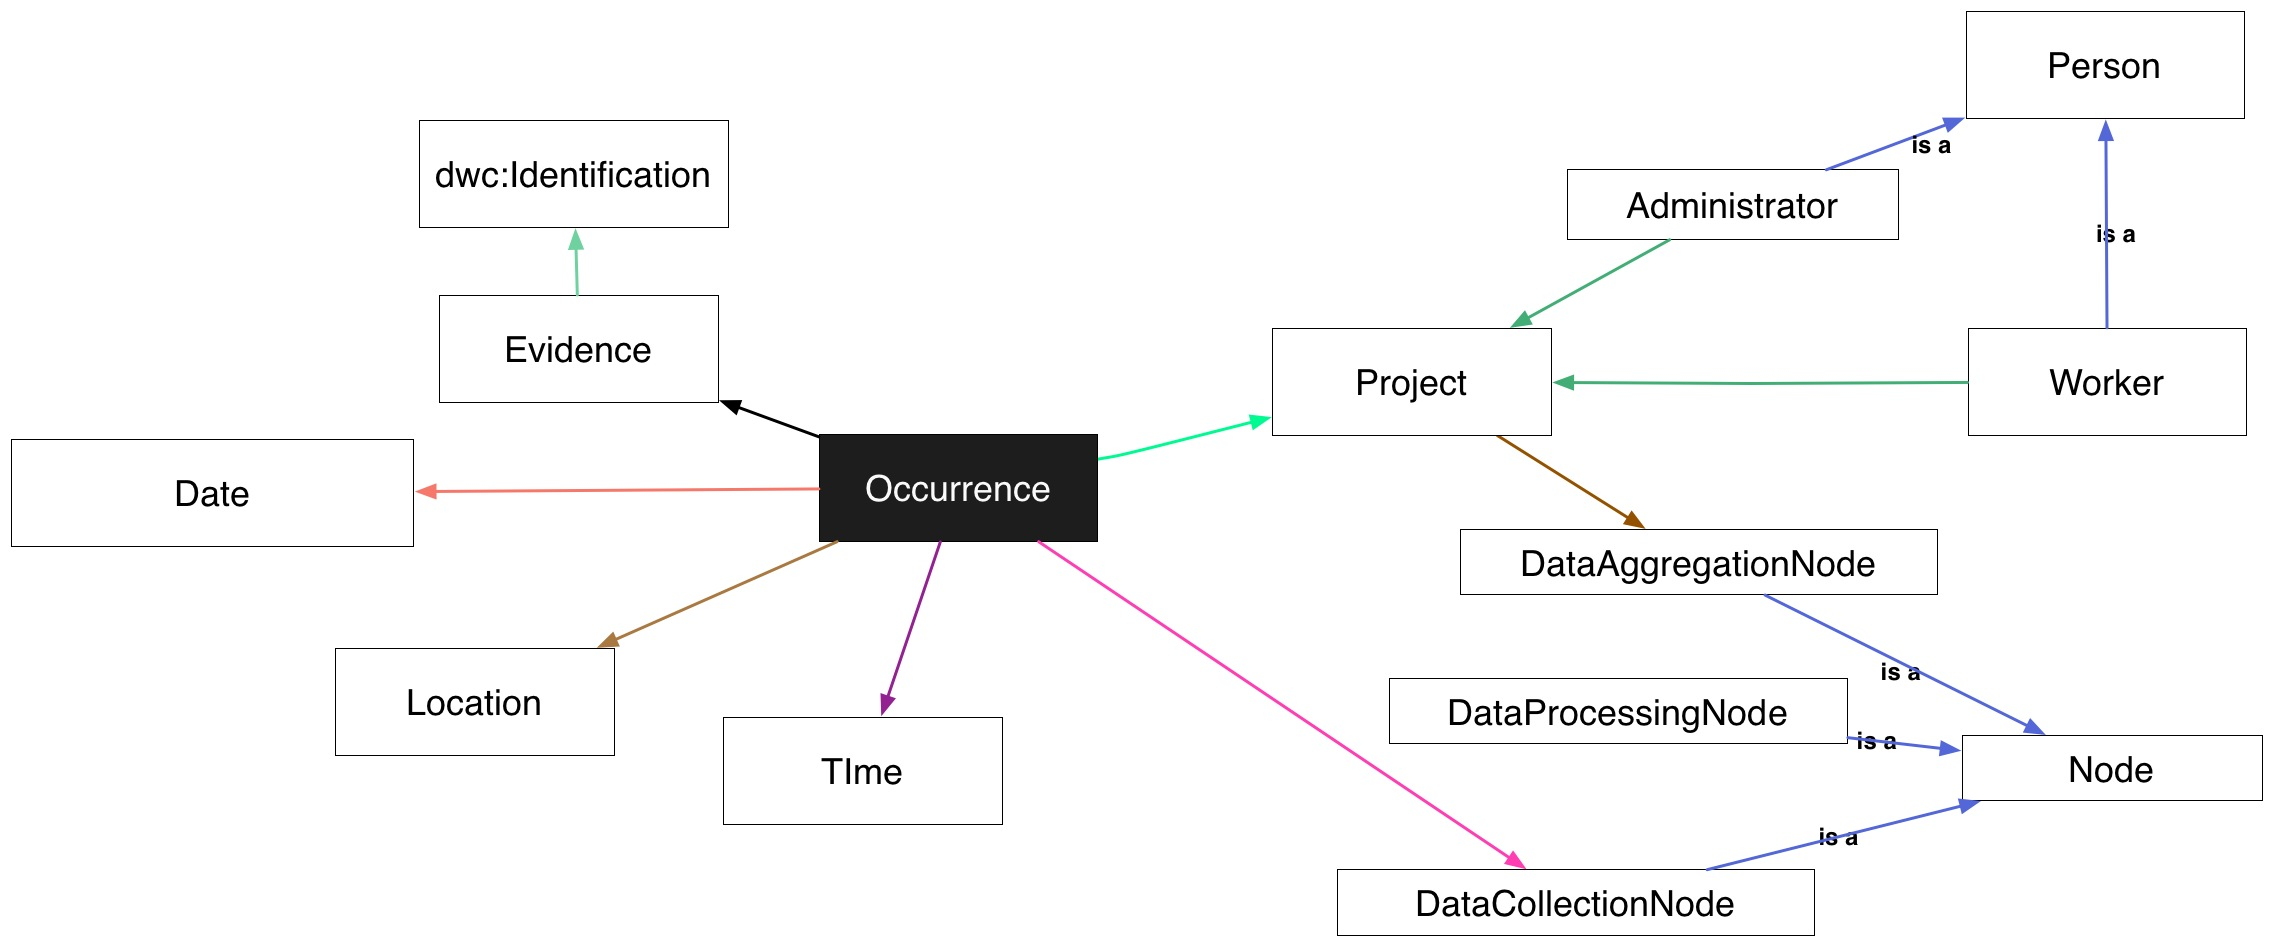
\includegraphics[angle=90]{Chap5/figures/khas_base.JPG}}
    \caption{K-HAS Base Ontology}
    \label{khas_base_ont}
    \end{figure}



\subsection{Build the Ontology - Code}
Once the concepts had been identified (and agreed upon), the ontology must be coded. We used Protege 4.2.2 \cite{Noy2000a} and implemented K-HAS in the Web Ontology Language (OWL), creating a core file that could be expanded; should we need to import existing ontologies.

\subsection{Build the Ontology - Integrate Existing Ontologies}
Our proposal for K-HAS is focused on scientific observations. Because of this, the focal point of our existing ontology research is of ontologies that are centred around scientific observations, this allows us to create a more generic ontology that is still able to capture all of the semantic details associated with a wildlife observation.

As explained in Section \ref{bg}, our research of existing ontologies covered two categories: observation-centric and sensor-centric. We identified ontologies, within multiple domains, that satisfied many of our requirements for K-HAS, but not all. Using the core concepts outlined in Section \ref{buildcapture}, we created a minimal ontology and used the results of our research to map K-HAS concepts to those that had already been identified.

During this process we found that we had determined concepts that mapped to existing ontologies, but may not share identical structures, or even the same name. For example, the OBOE ontology describes the concept of an occurrence, which is very similar to our occurrence and the occurrence in the Darwin Core-SW ontology. When we found these mappings, we used \textit{sameAs} relationship to form a link that allows data stored according to these existing ontologies to map directly to K-HAS. However, the structure of an OBOE observation is, as outlined in Section \ref{OBOE}, is more generic for all types of scientific observation and depicts the observation of an entity, containing a measurement of a particular characteristic. Whereas the structure of a Darwin Core observation is more limited to scientific observations of taxa which allows it to have more predefined terms, such as location, species name and the evidence for the recorded individual. Because of this, it was difficult to create a structure that encapsulated both OBOE and Darwin Core due to the generality of an OBOE observation compared to the more specific structure of DwC.

Research showed that Darwin Core maps to K-HAS' requirements more completely, as well as the fact that there has been work to represent Darwin Core Observations in OBOE \cite{dwc_oboe}, K-HAS occurrences map directly to Darwin Core and elements that are similar to OBOE have been linked by the \textit{sameAs} relationship. This does mean that full OBOE observations cannot map directly, but K-HAS, and Darwin Core, occurrences can be converted, if necessary. However, using the terms in our ontology we can create a subset of an observation that does not include all of the terms defined in OBOE but can still map to all three ontologies.

For the sensor hardware of K-HAS, we found that the SensorML ontology maps directly to our concepts and we also realised that we did not need to recreate concepts that may already exist in popular ontologies outside of the domain spaces we researched. For example, the Friend of a Friend (FOAF) ontology \cite{Document2010} is an ontology designed to create machine-readable pages that describe people, so it is more logical that K-HAS reuses existing terms from popular ontologies to allow pre-existing data to be mapped with ease.

% INCLUDE TABLE TO MATCH TERMS TO EXISTING ONTOLOGIES??

\subsection{Extend theOntology}

Whilst researching popular ontologies, we became aware that some classes identified for K-HAS were not satisfied by what is currently available, these are prefixed with khas and shown in Figure \ref{khas_ont}. The final step for creating the ontology was to add these concepts to the linked ontologies, we call these \textit{extension concepts}, concepts unique to K-HAS which do not exist in any other ontology. These terms were linked to the unique layered architecture of K-HAS and we defined them within a new K-HAS namespace, changing our ontology from an alingment of existing ontologies to an extension of these.

The final ontology is shown in Figure \ref{khas_ont} and shows how each concept maps to existing ontologies. The figure shows that there were only five extension concepts unique to K-HAS that can be subclassed from the \textit{person} concept in the FOAF ontology and \textit{node} in the SensorML ontology.

    \begin{figure}[h]
    \centering
        \scalebox{0.14}{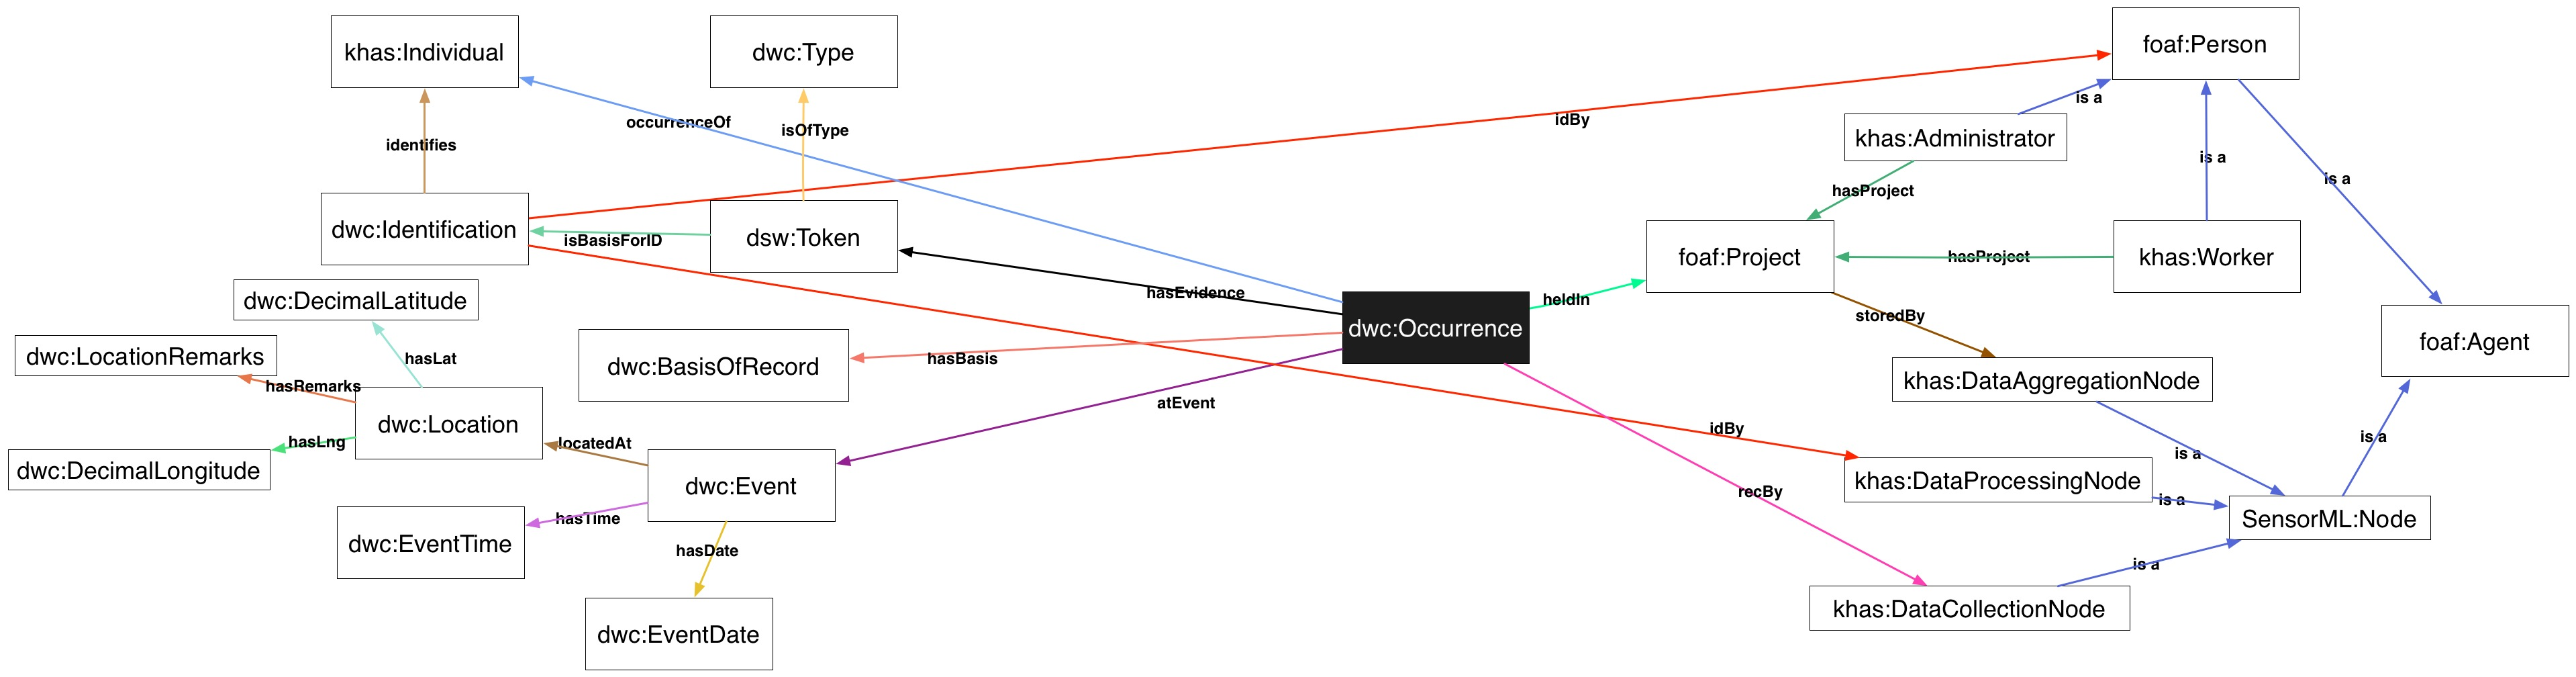
\includegraphics[angle=90]{Chap5/figures/khas_ontology.JPG}}
    \caption{K-HAS Ontology}
    \label{khas_ont}
    \end{figure}
    
\section{Evaluation}

Uschold and King's ontology development method does not explain how to evaluate the created ontology and much of the literature describes a number of methods that can be employed, \cite{Brank2005} outlines a number of different evaluation techniques and separates them into categories. These categories are listed below:
\begin{enumerate}
	\item Comparing the ontology to a `golden standard'.
	\item Using the ontology in an application and evaluating the results.
	\item Comparing the ontology with a collection of documents from the domain to be covered.
	\item Manual evaluation by humans to test if the ontology meets a set of predefined criteria.
\end{enumerate}

The last category mentioned is similar to the method in Section \ref{method:eval} that uses the competency questions to determine the effectiveness of the ontology. Because there is no agreed method,we have evaluated K-HAS by testing it in the application it was developed in (Protege), mapping it to existing documents within the intended domain and ensuring that it can satisfy all of the competency questions we outlined in Table \ref{tab:comp_qs}.

\subsection{Using the Ontology in an Application}
We developed the K-HAS ontology in Protege, a Java based ontology editor, that also provides the functionality to reason over the ontology and check for inconsistencies. Using the Hermit reasoner that is built into Protege, the ontology was determined to be logically consistent.

To confirm the validation provided by Protege, we also used a web-based ontology validation tool, called the OntOlogy Pitfall Scanner (OOPS), that scans an ontology for common errors, such as defining incorrect inverse relationships or using recursive definitions, that can occur during the development phase \cite{Poveda-Villalon2012}. The results of this tool showed that no pitfalls had been detected.

We have a customised build of K-HAS running that receives data from a variety of sources and stores it in a MySQL database that allows users to classify through a web site. The schema of the database maps to our ontology, scientific observations are received, unzipped and stored in the relevant fields in the database. Using real sensed data, we have successfully stored over two hundred occurrences and mapped existing DwC occurrence to K-HAS.

\subsection{Competency Questions}

In Table \ref{tab:comp_qs} we have identified some basic competency questions that we expected K-HAS to be able to satisfy with the concepts we had identified, Table \ref{eval:comp_qs} shows how the original questions are satisfied by K-HAS. We have mapped the terms we originally used to the terms used in K-HAS (and the linked ontologies) and shown the concepts involved with each question, as well as the relationships linking them.
\begin{table}[!t]
\caption{Competency Questions} 
\begin{tabular}{ p{5cm}p{5cm}p{5cm}}
\hline
\textbf{Competency Questions} & \textbf{Concepts} & \textbf{Relationships}\\ 
\hline
Find all \textbf{Occurrences} of an \textbf{Individual} & Occurrence; Individual & Occurrence occurrenceOf Individual \\
Find all \textbf{Occurrences} of an \textbf{Individual} at a \textbf{Location} & Occurrence, Token, Individual, Location, Identification & Occurrence hasEvidence Token \\ 
& & Token isBasisForID Identification \\ 
& & Identification identifies Individual \\
Find all \textbf{Occurrence} within a specified \textbf{Date} and \textbf{Time} range & Occurrence; Event; Date; Time & Occurrence atEvent Event \\
& & Event hasTime Time \\ 
& & Event hasDate Date \\
Find all \textbf{Data-Collection Nodes} that have recorded an \textbf{Occurrence} of an \textbf{Individual} & DCNode; Individual; Occurrence & Occurrence recordedBy DCNode \\
& & Occurrence occurrenceOf Individual \\  
Find all \textbf{Locations} of an \textbf{Individual} & Occurrence; Individual; Event; Location & Occurrence occurrenceOf Individual \\ 
& & Occurrence hasEvent Event \\ 
& & Event locatedAt Location \\
Find the storage location of a \textbf{Project} & Project, Data Aggregation Node & Project storedBy DataAggregationNode \\ 
Find all \textbf{Projects} containing an \textbf{Individual} & Individual, Project; Occurrence & Individual occurredIn Occurrence \\ 
& & Occurrence heldIn Project \\
Find all \textbf{Persons} involved in a \textbf{Project} & Person; Administrator; Worker; Project & Administrator hasProject Project \\ 
& & Worker hasProject Project \\
Find all the \textbf{Evidence} that supports an \textbf{Occurrence} & Occurrence; Token & Occurrence hasEvidence Evidence \\
Find all the \textbf{Types} of evidence that supports an \textbf{Occurrence} & Occurrence; Token; Type & Occurrence hasEvidence Token \\ 
& & Token isOfType Type \\
\hline 
\end{tabular}
\label{eval:comp_qs}
\end{table} 

The table shows that all of the competency questions outlined in Section \ref{ident} have been satisfied by the final ontology and each concept used maps quite easily with little to no change.

\subsection{Comparing the Ontology with a Collection of Documents}
Within the domain of scientific observations, Darwin Core is a popular choice for observations of wildlife and plants, it was because of this that we chose to use many of the pre-existing concepts from Darwin Core in K-HAS. 

In the data driven approach suggested by \cite{Brewster2004}, a corpus of documents, related to the domain that the ontology covers, and the keyword content is matched with the terms used in the ontology. Because Darwin Core observations are structured into archives of files, explained in Section \ref{bg:dwc}, we evaluated the K-HAS ontology by combining the approach of comparing a corpus of documents related to the domain with human evaluation of ensuring an ontology met a set of requirements to create a method that ensured existing scientific sensed observations could be mapped to K-HAS with little to no modification.

As we have previously explained, an archive of Darwin Core files consists of a minimum of 3 files: a metadata file that contains information about the creator of the archive and the project it relates to (eml.xml), a metadata file that describes all of the files that contain the occurrence and the fields within them (meta.xml) and a csv file that contains the data relating to the occurrence itself. Within the archive, the core files that need to be mapped to K-HAS are the meta.xml and eml.xml files as this allows us to store what and who.

We used files from a DwC archive made available online to extract the terms associated with an occurrence and we mapped these terms to K-HAS concepts, the results can be seen in Table \ref{tab:dwc_eval}.

\begin{table}[h]
\caption{Evaluation of K-HAS against Darwin Core Occurrence Terms} 
\begin{tabular}{ p{5cm}p{5cm}p{5cm}}
\hline
\textbf{Darwin Core Term} & \textbf{K-HAS Concept}\\ 
\hline
occurrenceID & Occurrence \\
basisOfRecord & Basis of Record \\
recordedBy & Person/Node \\
associatedMedia & Token \\
eventDate & Event Date \\
eventTime & Event Time \\
locationId & Location \\
scientificName & Individual \\
identifiedBy & Person \\
dateIdentified & Identification \\
\hline 
\end{tabular}
\label{tab:dwc_eval}
\end{table} 

Each term within a Darwin Core observation maps to K-HAS with only a few changes to the terms, while the definitions do not change. As K-HAS is an alignment ontology, there are extra concepts that do not map to Darwin Core, but can encapsulate each occurrence. For example, a project in K-HAS can contain many occurrences. As previously mentioned, \cite{dwc_oboe} shows how a DWC archive can be represented in OBOE, which means that it would not be too complex to map an OBOE observation in K-HAS.

\section{Conclusion}

In this chapter we have presented an ontology for the K-HAS architecture and described our methodology for development, as well as showing that existing ontologies are not complete enough to cover our requirements for K-HAS. The K-HAS ontology we present is an alignment of ontologies that are spread across multiple domains and provides a complete solution for a sensor network that deals with scientific observations and we believe this is the first extension ontology that combines sensor-centric and observation-centric ontologies. We have also extended this alignment to include concepts that model the unique features of K-HAS, but this ontology should be suitable for any sensor network that deals with observations.

Our evaluation has shown that the ontology is logically consistent and that existing scientific observations, in other formats, can be mapped across to K-HAS with few changes. The competency questions we identified during the design phase of the ontology can all be satisfied by the resulting ontology and our K-HAS network currently stores data with a schema that follows the design of this ontology.

In the future, work would be done to make the Darwin Core terms more modular and users will then be able to `plug in' their occurrence structure of choice. Currently, this ontology has been developed with the scientific observations of our motivating scenario in mind. The modular design allows it to be adapted to suit observations with different structures. The K-HAS, FOAF and SensorML modules can all be reused in almost any WSN but not all networks will be tasked with recording individuals. In these cases, DwC (and some K-HAS) terms would need to be replaced with terms suited to the task of the network, such as flood monitoring.


\chapter{Deployment in the Malaysian Rainforest}
	In this chapter, we detail the design and deployment of a modified K-HAS in the Malaysian rainforest. We also highlight the issues we experienced deploying the architecture in a humid, dense rainforest for use by those without domain knowledge of WSNs.
	
	Experiments carried out in the rainforest had already shown that the range of wireless communications could be reduced by up to 80\% and we expected that the lifetime of nodes in such conditions would be affected.
	
	Yearly visits were made to the Danau Girang Field Centre (DGFC) to test different nodes, gather knowledge and trial iterations of K-HAS. The first visit showed us just how much the rainforest affected communications, but also allowed us to gather knowledge from researchers and cameras that had previously been deployed. Subsequent visits were then used to test our own nodes and software, based on the knowledge we had gained from the first visit. We developed K-HAS with a view to deploying it in Malaysia, however, it soon became clear that our design was  beyond what was currently available, as well as the time constraints.
	
	Developing a camera with both wireless and processing capabilities, as well as being waterproof, proved to a be an extremely difficult task, while wireless wildlife cameras were already commercially available with range much higher than what our experiments had yielded. This could be because of their test environments being places such as American forest with less dense foliage, lower canopies and much lower humidity and using wireless technologies that are not licensed for worldwide use. For our own node designs, we attempted to use various node types connected to a camera, such as the Raspberry Pi and Waspmote nodes; both yielded problems with mounting an SD card that was readable by both camera and node. At the time, we were unable to create a camera combined with a node that could be left untouched for months at a time in a rainforest.
	
	However, we still needed to implement a network to evaluate our approach, thus we developed a modification to the K-HAS that utilised the latest commercially available hardware to provide an architecture that provides similar capabilities. Because these changes were made due to issues with deployment in Danau Girang, we chose to name it LORIS, after a famous animal in Malaysia. A Slow Loris is a small, nocturnal primate commonly found in South and Southeast Asia but in our context it is an acronym that stands for Local-knowledge Ontology-based Remote-sensing Informatics System.
	
	LORIS has been developed specifically for the Malaysian rainforest, our motivating scenario and, as such, much of the hardware and software has been implemented to reflect this.
	
	The rest of this chapter is structured as follows. Section \ref{loris:arch} highlights the changes we had to make from K-HAS and explains the hardware used at each tier. Section \ref{loris:dep} explains how we planned and deployed the network and Section \ref{loris:res} details the results from the deployment in Malaysia.
	
	\section{ Deployment Architecture}\label{loris:arch}
		The aim of LORIS was to keep as much of the architecture of K-HAS as possible and reuse the ontology without the need for modification; serving as a form of validation. In order to do this, we identified the tiers of the network that could be deployed in the rainforest, given the hardware and wireless constraints, and the areas that needed to be addressed. Regular power and cheap computers with good knowledge-processing capabilities meant that DA nodes were simple to deploy and, with the growth of powerful microcomputers like the Raspberry Pi, DP nodes were also in abundance. However, finding a reliable camera that could integrate with a node capable of processing observations that was also reliable enough to withstand the humid rainforest proved to be difficult.
		
		\subsection{Data Collection}
				Experiments were run yearly in Malaysia to test the performance of variations of hardware. As covered in Section \label{tech:wifirange}, the first year involved testing the range of Wi-Fi with an IGEP board. The limited range of 30m meant that, despite the high transfer rate, it was not possible. Wi-Fi was not designed for use in resource-constrained sensors, so the power consumption of the radio meant that it limited the lifetime of the node.
				
				The following year, we used the Digimesh protocol, explained in Section \label{tech:digimesh}, which provided a longer range and was developed for use in sensor networks.  While the range was suitable for the rainforest, it was not as much as we had anticipated. The other difficulty proved in mounting an SD card on two devices at the same time, the existing wildlife cameras and our Waspmote nodes, without causing corruption from read/write clashes.
				
				From these experiments, we began to look into commercial alternatives that combined both the node and the camera. The most usable solution we found was the Raspberry Pi coupled with a camera attachment \cite{Sarajevo2014}, but it was not ready for use in the Malaysian rainforest or to be used for an extended unsupervised period. Existing wildlife manufacturers were then looked into and we found that wireless cameras had been manufactured, but they had no local processing capabilities and had not been used much in research. Based on these findings, we used Buckeye X7R cameras \cite{Buckeye}. Using the same Digimesh protocol as the Waspmote, they had a tested range of 1 mile and their casing had been developed to withstand harsh environments. The 1 mile range was tested in a more open woodland in the US but the higher quality components used, as well as their modifiable antenna supported our theory that we would achieve better range with their cameras.
				
				We expected to achieve around 800m of range and these proved to be suitable DC node replacements, despite the fact that we had to forgo local processing or the storage of any local knowledge.
		\subsection{Data Processing and Aggregation}
				Because our DC nodes were wildlife cameras that did not have any knowledge processing capabilities, and because our DC node sites were near enough to the field centreß, we combined the DP and DA nodes into one machine stored at DGFC, that contained both a Digimesh radio and an Internet connection. The benefit of using commercial grade hardware was the software that accompanied it; remote management and configuration software allowed users to modify the settings on each camera, as well as handling the retrieval of images from every node deployed. EXIF tags written to images could be modified, as well as how many images were captured for each observation. The software had been created to be used by those without any specialist knowledge and was easily used by researchers in the field centre.
				
				Each observation was saved into a directory that matched the ID of the camera it originated from and this meant that the existing software used in K-HAS could be used without modification. Sensor middleware, such as GSN, is running on the same machine and virtual sensors listen for changes in each directory; where each virtual sensor represents a deployed camera.
				
				When new observations are detected, Drools runs on the images to start metadata and EXiF processing. Some rules had already been extracted from the processing of 120,000 images collected from our yearly visits to DGFC; other rules had to be added by users of the WSN. When an observation had been processed, rules were run once again to determine if a match could be made to existing projects and, if so, who should be notified.
				
				The web interface for classifying and viewing all observations was accessible by those within DGFC, as well as uploading rule files and new locations. Using this interface proved to be easier for those without a WSN background and the GSN interface had a steeper learning curve.	Figure \ref{fig:loris} shows the basic metadata of an observation, outlining where it was captured and when; as well as the images themselves.
				
				\begin{figure}[h]
				\centering
				\includegraphics[width=\textwidth]{Chap6/figures/loris}
				\caption{LORIS Web Interface}
				\label{fig:loris}
				\end{figure}
				
	\section{Deployment}\label{loris:dep}
		In June of 2013, a three week visit was made to Danau Gurang, with three Buckeye cameras and the software required to deploy LORIS. The network was first tested within the field centre and one of the Buckeye cameras had been broken during transport, giving us only two cameras. Due to the protected nature of the forest, we were unable to nail any cables to trees to use the high gain antenna and it was not possible to use the cables without first securing them, because animals tampering with cameras was a common occurrence.
		
		For the initial week of the deployment, we wanted to test the robustness of the network before focussing on the data. This meant placing the cameras in locations where they would be triggered often and in an area where they would be affected by rainfall and humidity. Figure \ref{cam_locs} shows the locations of the cameras during both of the weeks that it was deployed. Buckeye 1 was deployed for the first week along the main path leading to the field centre from the river, this experienced the most traffic due to the number of researchers present at the time. 
	
	    \begin{figure}[h]
	    \centering
		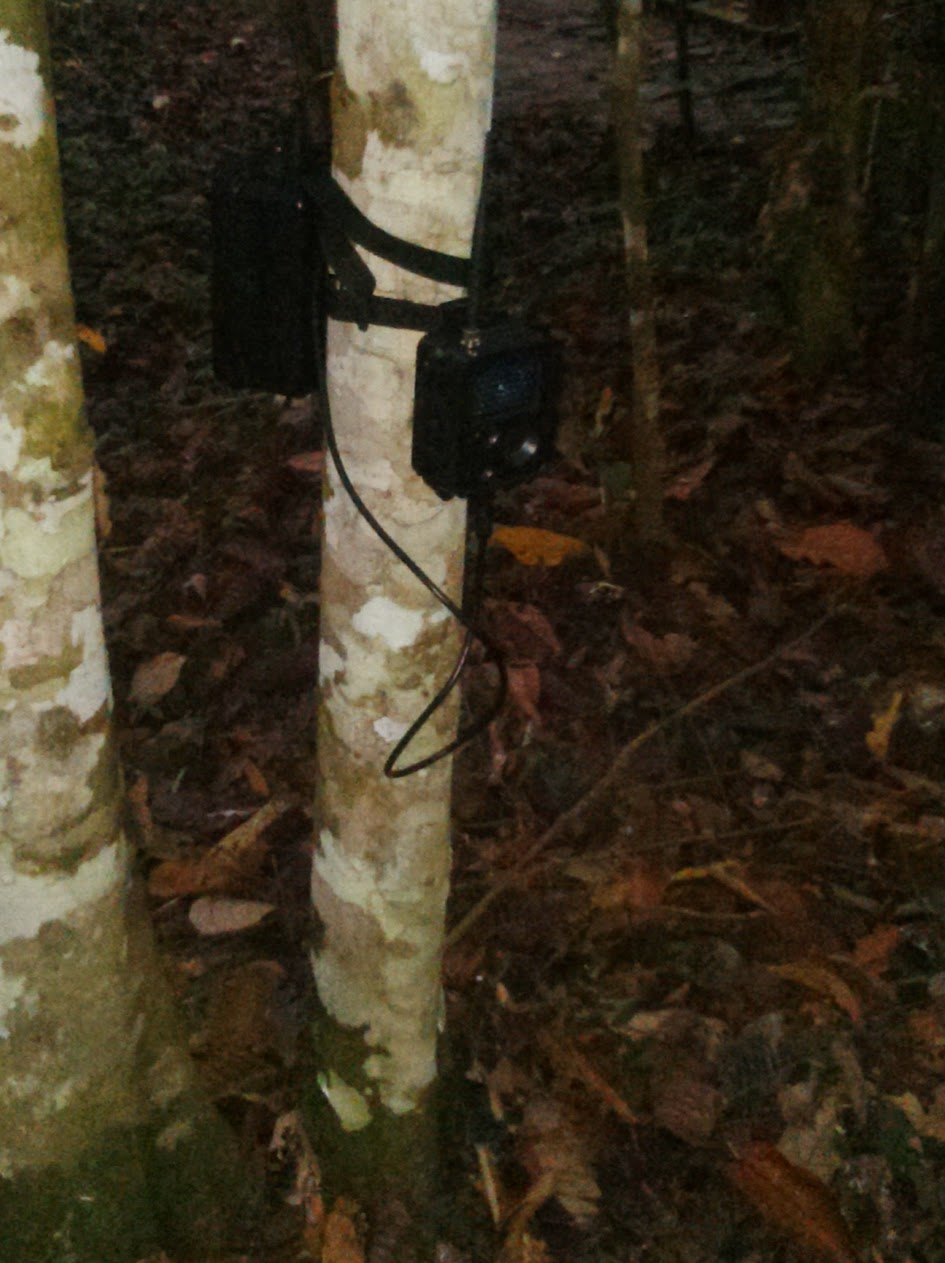
\includegraphics[width=\textwidth]{Chap6/figures/buckeye}
	    \caption{Camera Locations Around Danau Girang}
	    \label{cam_locs}
	    \end{figure}
	
		\subsection{Direct Connection}
		For six days, we tested two Buckeye cameras that were near enough to the field centre to maintain an active connection to the base station. This meant that no hopping was involved and cameras were not reliant on each other to transmit images. Buckeye 1 was placed on a main path that guaranteed human foot traffic and Buckeye 3 was placed on a trail in the forest that, while experiencing minimal foot traffic, was expected to yield small mammals and birds.
		
		For the duration of the six days, the cameras did not report a drop in battery levels and a total of 1076 images were sent. Buckeye 1 was in a more open environment, despite being further away, and average speeds of 4KB/s were achieved. 
		
		Transmissions from Buckeye 3 were significantly hampered by the dense forest that it was surrounded by, as well as the fact that a low-gain antenna was used. We also speculate that the field centre itself acted as a barrier to the signal, as the base station was located on the opposite end. Because of this, we experienced an average speed of 1.2KB/s, taking around three minutes to receive an image. This is consistent with experiments conducted in previous years where dense, humid forest has led to a decreased range of, up to, 78\%. Lower frequencies do experience a longer range, but the data rate is significantly impacted.
		
		\subsection{1-Hop Network}
		For a further five days, Buckeye 1 was moved further into the forest and Buckeye 3 was set up as a routing camera that forwarded images onto the base station, 63 images were taken during this period.
		
		The location of the moved camera is also shown in Figure \ref{cam_locs}. As was expected, the traffic of the network reduced significantly when the cameras were moved from the main path, with almost all 63 pictures being of animals. Due to animals moving a lot faster than humans, the number of pictures taken per trigger was increased to two, this would ensure network traffic was not overwhelming while increasing the chance of capturing the subject.
		
		Surprisingly, the speed of transmission from Buckeye 1 was faster than Buckeye 3, despite being routed through it, with an average speeds of 1.8KB/s.				
		\section{Results}\label{loris:res}
		Deploying a network for two weeks is not a robust experiment and does not show that LORIS can withstand months of running without human intervention. However, it does serve as a proof of concept that, using commercial hardware, a modified K-HAS network can be implemented and utilise the knowledge of its environment.
		
		The pictures of humans from the first six days are not of use for the current motivating scenario, focussed on animals in the rainforest corridor, but one could see this network also being tasked to warn the authorities of hunters in restricted areas of the rainforest. However, the images we have of animals, while few are animals of interest due to the proximity of the cameras to humans, were processed and used to create templates for future observations. 
		
		    \begin{figure}[h]
		    \centering
			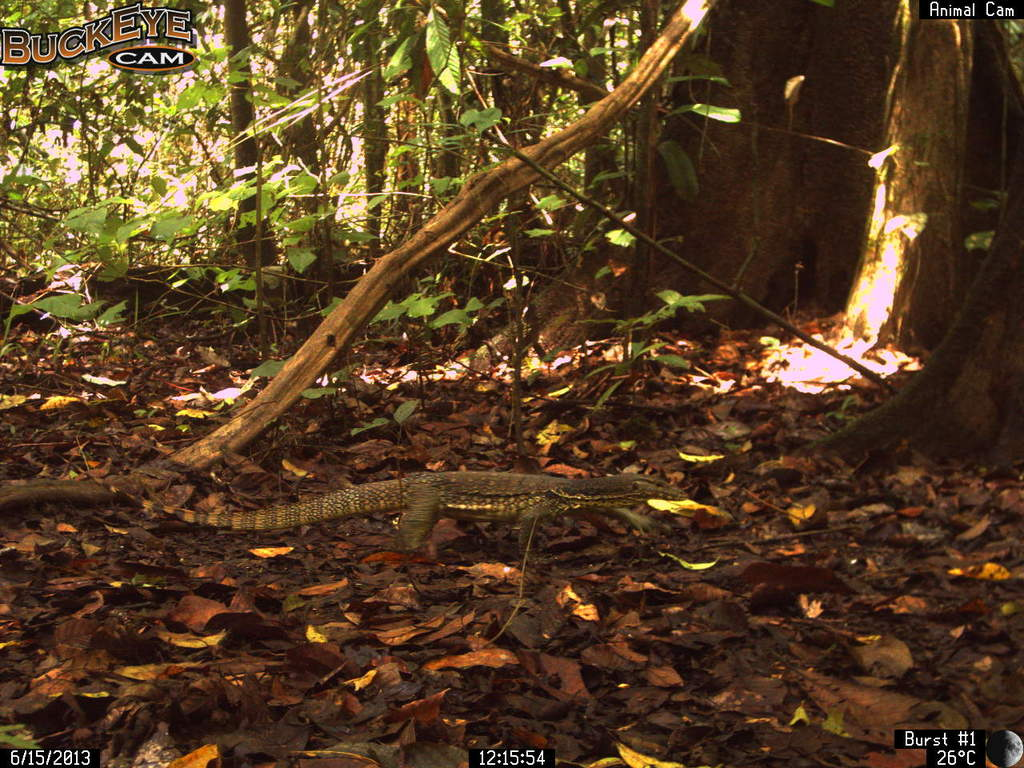
\includegraphics[width=0.65\textwidth]{Chap6/figures/buckeye_img}
		    \caption{First Image of Lizard by Buckeye 3}
		    \label{buckeye_img}
		    \end{figure}
		
		More interestingly, we were able to infer further rules from the short deployment that helped us to narrow down the choice of animals to match to based on the time of day and location. For example, Figure \ref{buckeye_img} shows a lizard crossing the path of Buckeye 3 in the middle of the day and Figure \ref{buckeye_img_2} shows the lizard walking past in early afternoon on a different day. This allows us to encode a window of time  in which the lizard is more likely to appear onto the static knowledge base of DC nodes or, in the case of LORIS, onto the DA/DP node. Images an hour later were captured by the camera, showing the lizard walking in the opposite direction. While this was not every day, and the deployment time was too short to establish a pattern, it does help us to infer that a lizard passing by in early afternoon is likely to walk the same path approximately an hour later.
		
		    \begin{figure}[h]
		    \centering
			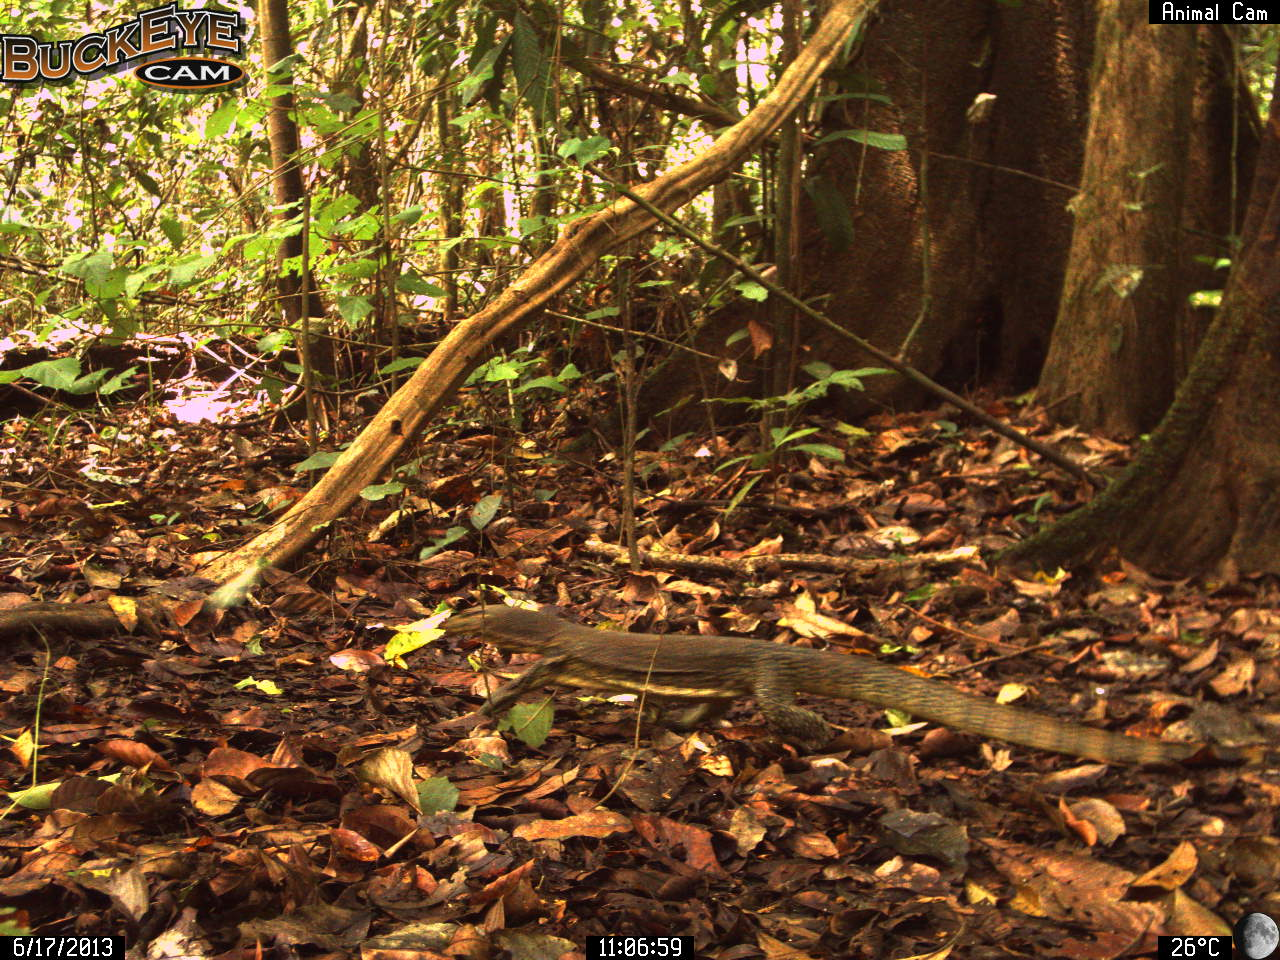
\includegraphics[width=0.65\textwidth]{Chap6/figures/buckeye_img_2}
		    \caption{Second Image of Lizard by Buckeye 3}
		    \label{buckeye_img_2}
		    \end{figure}
	
	\section{Rules}
		This section explains the rules used in LORIS and K-HAS in more detail, to highlight how classifications are made as well as how nodes in the network are monitored. Any examples made here relate to our motivating scenario. The rules on each node are a vital way of encoding local knowledge and a practical use to show how local knowledge, from users or previously sensed data, can be used classify newly sensed data.
		
		As highlighted in Section \ref{arch:kb}, K-HAS uses the Drools rule engine, a Java based rule management system that uses forward chaining based inference. Forward chaining starts with some data, in our case a set of images, and uses inference rules to extract more data. We use this method to make meaningful inferences from properties of the sensed data. For example, an image taken at 8pm could be run through Drools and an inference rule will tell the system to start by looking for nocturnal animals.
		
% 		\subsection{Data Collection}			
% 		As explained in Section \ref{khas:dc}, DC nodes are unable to run the Drools engine and instead utilise static rules that are encoded at the time of deployment. Instead of utilising forward chaining to draw a single conclusion, these rules are executed one by one and the outcome of one does not affect the outcome of another. An example of such rules could be a rule to determine the time of day that an image was captured (such as morning, afternoon, evening or night) or a rule to determine what animals it is more likely to be based on the temperature and location of the node, shown in Listing \ref{lst:dcrule}. No rule engine is used by the DC node and the rules are executed in the code before the observation is archived and sent on.
		
% \begin{lstlisting}[caption=Encoded Data Collection Rule, label=lst:dcrule, breaklines=true]
% 	if img.temp > 32 && img.temp < 38 then
% 	classification.potentialAnimals = [clouded_leopard, malay_civet, sun_bear]
% 	if img.time > 1800 && img.time < 0500 then
% 	classification.animalBehaviour = nocturnal
% \end{lstlisting}
	
	\subsection{Data Processing and Data Aggregation}
		The increased knowledge-processing capabilities allow DP nodes to run a complete implementation of Drools, this means that forward chaining can be used and the knowledge base is dynamic, i.e. it can be updated whilst the network is deployed. 
		
		Rules are written in \textit{drl} files that are loaded into a knowledge session. Sessions, as well as the firing of rules, are handled by the Java code. The benefit of using Drools with a Java based middleware, such as GSN, allows the simple integration of the two technologies, allowing a sensor class in GSN to insert an archive into the session and run the rules. When sensed data is received from a DC node, it is unarchived and Drools is run on the DwC files describing the original observation, the metadata, the originating DC node and the knowledge base of the DP node.
		
		Listing \ref{drools:dp} shows an example of some more simple rules that would be contained within the knowledge base. In this file, the rules use existing local knowledge with the properties of the observation to infer the contents and then update the DwC archive, or return suggestions as to what the contents may be. For example, the \textit{Clouded Leopard Ridgeline} rule uses the location ID of the camera to match with a human description and uses local knowledge of the area and global knowledge of the time to infer that the image may contain a Clouded leopard.
		
		\lstinputlisting[caption=Drools Rule File, label=drools:dp]{Chap4/listings/rules.drl}
		
		These rules are very simple and only scrape the surface of the local knowledge that can be utilised, as well as how DwC archives can be effectively used to carry the data of these inferences, but it does show that Drools is a powerful rule engine and that these rules can be extended further to make full use of the knowledge base. 
		
		DA nodes use the same rule engine as DP nodes but rules are used for the post-processing of Darwin Core archives. For example, when a classified archive is received from a DP node, Drools is run to check if the classification matches an existing project. If it does, then it searches for those that are subscribed to the project and notifies them via their selected medium. Drools can also be used to monitor the nodes deployed in the network and check their status. Rules are run to check for archives from DC nodes and, if a node has not sent an archive in a set number of days, then administrators are informed that it may have run out of battery.
		
		More importantly, rules are vital for the exchange of knowledge between nodes in the network. If a user classifies an observation on a DA node, then rules are fired that identify the DP node that sent it and update the knowledge base, on the original DP, so that the image template it uses in future classification matches the one identified by the user.
		
		\subsection{Existing Data}
			Throughout our visits to Danau Girang, we collected local knowledge through field work and interviews with the researchers based at Danau Girang. As well as this, we collected classifications made by the researchers for images that had been taken during camera deployment. Using these data, we have extracted patterns in animal movements in order to create some basic rules for the DC and DP nodes. In this section, we will describe the data we have and the methods used to extract rules.
			
			\subsubsection{Semi Structured Interviews}
			On our final visit to Danau Girang, we designed a set of 14 semi structured interview questions that we asked to ten researchers based at the field centre, with the majority working on different projects. We used these questions to gain insight into common trends between projects and patterns recorded about the animal subjects. A subset of the questions have been listed below:
			
			\begin{itemize}
				\item What species are you looking at?
				\item Do you have specific sites that you look into?
				\item What specifics do you know about the target species?
				\item Do others use your research? If so, how?
			\end{itemize}
			
			These questions have been designed to be as open as possible to allow the interviewees to provide as much detail as they wish, or even transition to a different topic. The interviews were recorded and later transcribed to text. We then used a software package called Dedoose \ref{REFERENCE}, which is an online tool that is used for performing qualitative analysis on text based documents. Uploading our documents to the service allowed us to manually review the responses to each question and highlight, or `tag', excerpts of interest and link to other excerpts that had either been mentioned by another interviewee; or were related to other comments. Each excerpt was tagged with the subject it was discussing, for example, a comment on the accessibility of an area of the forest during certain times of the year were tagged as \textit{local knowledge}. The excerpts were combined and exported into a CSV file that detailed who the interviewee was, the content of the excerpt and the tag.
			
			This method allowed us to gain knowledge we would not have learnt from our short time at the field centre, these face to face sessions gave us insight into patterns and observations that had been made by researchers who have been based at Danau Girang for many years. An example of this is the global knowledge of the sleeping patterns of Clouded Leopards. It is widely accepted that they are nocturnal however, the camera trapping project has shown that their sleeping patterns around Danau Girang do not support this and they have been seen throughout the day and night. This could be due to the human impact, availability of prey or even the climate of the area, but, if researchers had just used this global knowledge then they would have seen fewer Clouded Leopards. Similarly, if we had used a rule to only look for Clouded Leopards at night, then a lot of images would have been misclassified. While it cannot be directly encoded, this is an example of local knowledge overriding global knowledge.

			While we were not able to construct a full set of rules from these findings, the results have provided support for patterns extracted from existing data that has been classified by researchers, which we discuss further in the next section. 
			
			\subsubsection{Existing Data}
			When images are manually collected at Danau Girang, researchers process each image set and they have recently been recording the classifications. However, these classifications are only being recorded for currently ongoing projects and other images are ignored. During one of our visits, we collected a CSV file of 2650 confirmed classifications made by researchers. The data had not been cleaned and multiple users had used different names for the same species, we cleaned the data manually and matched it with the images in our database.
			We then used the classifications for each species to determine any patterns by analysing the details recorded for each observation, which are listed below:
			\begin{itemize}
				\item Time
				\item Date
				\item Location
				\item Temperature
				\item Moonphase
				\item Classification
			\end{itemize}
			
			SQL queries provided these details for each species and we recorded patterns that could be identified. For example, if a Samba Deer was only spotted between the hours of 7pm and 4am then we could write a rule that the species is nocturnal. More detailed rules can be created if there are patterns across multiple details. A species that is only spotted in two of the twenty sites between the hours of 7pm and 4am means that nodes with local knowledge can make accurate classifications without the need for image processing. However, these rules are based on large amounts of data collected from an active, or previous, deployment. DC nodes in their early deployment stages would not have the data to make such detailed rules.

				\begin{lstlisting}[breaklines=true, caption={Example Rule created from Existing Data}, label={imp:lst:rule1}]
if TIME > 1500 and TEMP <= 26:
    if TIME < 0000:
        if MOONPHASE <= 2:
            CLASSIFICATION = GOAT (25\% chance)
        if MOONPHASE > 2:
            if DATE in JAN:
                CLASSIFICATION = HUNTER (2.6\% chance)
				\end{lstlisting}
			
			Using the Weka package, we constructed a J48 decision tree and used the resulting model to create a collection of simple rules that could be run on a DC node. Figure \ref{imp:lst:rule1} shows a rule that was created from the output. This rule checks the time of capture for the observation, the temperature and the moonphase; which has been converted into a numeric values. If the temperature is less than 26 degrees and the time is between 3pm and midnight, then there is a 25\% chance of the classification being a goat. The if-statements are executed in order and the classification that matches the properties of the observation, and has the highest percentage chance, is forwarded to a DP node.
            
            Because the features used to generate the rules are available in every observation, and do not require any external information, DC nodes are able to process the series of if-statements quickly. This method of knowledge-processing comes at the cost of accuracy, when compared to using existing data, image processing and/or a dynamic knowledge base, but the speed and simplicity of these rules mean that they can be used by almost any node, regardless of computational capability.

		
	\section{Conclusion}\label{loris:conc}
	 K-HAS was developed, with the motivating scenario in mind, as an ideal, general-purpose network architecture that is able to utilise the knowledge of its environment. However, experiments to support the design and deployment of such a network within the timeframe of this PhD showed that the current technology was not ready to support a network that would run without human intervention for extended periods. LORIS is our more specialised, cut down approach that can be implemented using commercial hardware that is readily available, as well as software that we have open-sourced. 
	
	Our deployment in Malaysia has shown that local knowledge can assist with classifications and can be gained from even a few images collected within the first few days of deployment. Ideally, we would like to leave this network running for an extended period to infer rules from the sensed data and test the reliability of the network in harsh conditions. From both the visit and the deployment, we have offered evidence for the existence of local knowledge and provided a method that can be used to extract it from field experts. 
    
        The rules extracted from the interviews and classified data we collected while deploying LORIS can be used as a static knowledge base for DC nodes in the K-HAS architecture, or as the basic starting knowledge base for the DA node in LORIS. As more classifications are made to new sensed data, this same process can be used to create new rules for previously unrecorded classifications, as well as refine existing rules. 
	
	LORIS has shown that local knowledge can be used to enrich sensed data, and automate classification, when it has been received at the field centre, but we  maintain that K-HAS' aim of pushing local knowledge right out to the edge of the network makes a network more efficient and allow for a more timely delivery of important sensed data.  The main drawback of LORIS is that it relies on the chronological delivery mechanism used by the commercial cameras, whereas K-HAS can improve this mechanism by sending the data that it infers to be of a higher importance, rather than what was simply captured first.
\chapter{Simulation Experiments and Evaluation of the Architecture}
In this chapter, we present the results of simulation experiments developed to evaluate and explore choices offered by our K-HAS architecture. Using nodes with knowledge-processing capabilities to deliver interesting data quicker than a standard WSN, we have developed a simulation for our proposed architecture, K-HAS, as well as variations on the knowledge processing capabilities of the nodes at each tier.

The simulations were developed to determine whether K-HAS is the best mix of processing and collection nodes that maximises network lifetime while minimising the transmission time of interesting data. This was done by using a network structure, that matched our motivating scenario, and changing the knowledge-processing capabilities on each node at every tier; ranging from no knowledge on every node to the maximum knowledge-processing capabilities across the network. We aim to show that the more knowledge-processing capabilities that are pushed out towards the edge of the network, the more effective the network becomes at prioritising data that it believes to be interesting and delaying what it believes to be empty.

This chapter is structured as follows. Section \ref{sim:sim} describes the implementation of the network. Section \ref{sim:imp} outlines the results and Section \ref{sim:res} compares these with LORIS and the current solution in our motivating scenario. Section \ref{sim:conc} concludes our findings and highlights areas that require further experimentation.

\section{Simulation Environment}\label{sim:sim}

Using RePast Simphony \cite{Collier2003}, a agent-based network simulation tool developed in Java, we created a network to emulate K-HAS. RePast is an agent-based modelling system that allows for agents to be created and placed on a grid. Ticks denote a period of time and simulations can run for a fixed number of ticks, or until stopped. Ticks can also be used to schedule events, such as searching for neighbours, by calling methods that last for a set number of ticks, or begin at a particular tick. For example, a camera sensor node may be tasked with taking a picture every three hundred seconds. When the simulation reaches three hundred ticks (or six hundred, nine hundred, twelve hundred and so on), a scheduled event is run that would simulate the camera's capture of an image and transmitting it to an endpoint.
%train may take three hundred for it to arrive at its destination. When the simulation reaches three hundred ticks, a scheduled event could run that would open the train doors, make an announcement and so on.

RePast was chosen because we did not require the low level network configuration provided by other tools, such as NS2 \cite{mccanne1997network}, but we did need to modify and record the behaviour between nodes as they capture and process sensed data. RePast's event scheduling allows for nodes to be modelled as agents and the dynamic configuration allowed us to modify the simulations during run time. The aim of these simulations was to visualise how different knowledge-processing capabilities can affect the prioritisation and transmission time of observations, as well as the accuracy of their classifications. RePast allowed us to utilise existing Java code we were using in our K-HAS middleware and develop a base simulation that could be configured easily with XML files.

Agents were created, using the RePast SDK, and Java classes were used to manipulate their behaviour. Simple networks may only contain basic agents with only a few variations from those provided by RePast. However, for more complex networks, a hierarchy of agents is required and Java's inheritance can then be used to create subclasses of an agent.

A 2D space is used to display the grid and the simulation is run within RePast's own GUI. This GUI provides functionality such as editing the properties of classes, integrating with Matlab, taking screenshots and saving different configurations of the same network.

\section{Experiment Design}\label{sim:imp}
	While the aim of these simulations was to show the effectiveness of K-HAS over the current solution, we also wanted to determine if it was the optimal solution, in terms of delivery of interesting data and network lifetime. We believe that the ideal solution would be to attach nodes with high knowledge-processing capabilities to all cameras in the network, however the short battery life means that replacements would be made as often as the current manual solution, detailed in Section \ref{tech:motiv}.

	Throughout this chapter, we will be referring to nodes tasked with different purposes as the three definitions listed here:
	\begin{itemize}
		\item Sensing Node: A node that has been tasked with the captuing, and routing, of sensed data.
		\item Routing Node: A gateway node that is tasked with collecting, processing and forwarding sensed data.
		\item Central Node: A node with similar functionality to a typical base station, tasked with storing all sensed data and providing an interface to users.
	\end{itemize}

	At the routing and sensing tier, the degree of knowledge processing capabilities can range from the levels outlined below:
	
	\begin{itemize}
		\item No Knowledge (NK): The node possesses no knowledge processing capabilities.
		\item Minimal knowledge (MK): The node possesses basic knowledge processing capabilities and contains a static rule base (Section \ref{khas:dc}).
		\item High Knowledge (HK): The node possesses high knowledge processing capabilities and is able to process data, metadata and use a dynamic rule base (Section \ref{khas:dp}).
	\end{itemize}
	
	The higher knowledge-processing capabilities of HK nodes allow them to classify observations with a greater accuracy, but their battery life is much shorter than MK nodes due to their increased power needs (Section \ref{tech:hw}). In contrast, MK nodes can run for a longer period without requiring battery replacement. MK nodes, however, are unable to classify observations to the same level as HK nodes. While HK nodes can classify an observation as interesting or empty and, in our scenario, match to a species, MK nodes can only assume an observation is interesting using the image's metadata as they lack the capabilities to reliably determine whether an observation is empty or not. The scenarios we have implemented cover combinations of HK, MK and NK, in a twenty five node network. We use twenty five nodes because DGFC had a between twenty and twenty two active cameras during our first and second visits and we knew that the first implementation of the network would require a single endpoint. From this, we chose to use four routing nodes so that each could handle an equal number of sensing nodes, if they were all within range, and a single central node. Our experiments in Danau Girang were restricted to a smaller number of nodes, due to cost, but we expected to deploy a sensing node onto all of the active cameras. The hierarchical nature of the network is shown in Figure \ref{fig:sim} and explained later in this section. These scenarios were developed to determine which combination of MK, NK and HK nodes allowed for the greatest network lifetime, as well as the greatest accuracy when delivering interesting sensed data, and they have been outlined below:
	
	\begin{itemize}
		\item NK-ALL: Sensing and routing nodes possess no knowledge processing capabilities.
		\item MK-ALL: Sensing and routing nodes possess minimal knowledge processing capabilities.
		\item NK-MK: Sensing nodes possess no knowledge processing and routing nodes have minimal knowledge.
		\item MK-HK (K-HAS): Sensing nodes have minimal knowledge and routing nodes possess high knowledge. This scenario matches the K-HAS architecture we proposed in Chapter \ref{chap:arch}
		\item HK-ALL: Sensing and routing nodes have high processing capabilities.
	\end{itemize}

Before implementing, we designed the agents required based largely on the ontology proposed in Chapter \ref{chap:ont}. Using that, we created a hierarchy of nodes inheriting common properties from a node object. As previously mentioned, we had metrics on range and transmission times from previous experiments and the deployment of LORIS. We used these to create properties for each transmission medium that could be used by each node object. Table \ref{sim:tab:terms} shows how the K-HAS terms, introduced in Chapter \ref{chap:arch}, and LORIS terms, detailed in Chapter \ref{chap:imp}, map to the node types described above. The nodes used in our simulations map directly to the ontology.

\begin{table}[h]
\centering
\begin{tabular}{|l|l|l|}
\hline
\textbf{Network Type} & \textbf{Original Term} & \textbf{Maps To}          \\
\hline
K-HAS                 & DC Node                & Sensing Node + MK         \\
                      & DP Node                & Routing Node + HK         \\
                      & DA Node                & Central Node + HK         \\
LORIS                 & Buckeye                & Sensing Node + NK         \\
                      & DA and DP              & Routing/Central Node + HK \\
\hline
\end{tabular}
\caption{Mapping of K-HAS to Simulation Terminology}
\label{sim:tab:terms}
\end{table}

Using a Java library we developed for DwC archives during the implementation of LORIS (Section \ref{loris:arch}), we were able to implement DwC archives as the data standard in our simulations, this allowed us to model the prioritisation of sensed data, as well as the classification of observations, in the same way that an actual WSN would.

The structure of the simulation is as follows: The \textit{network builder} instantiates all the nodes, places them randomly on the grid and schedules events once the simulation has started. The nodes then use the properties of their transmission medium to find nodes in range and create a connection; depicted by a line between the node. The simulation uses metrics, such as the size of the image, extracted from the images taken at Danau Girang and the chance of an image being captured by a camera is based on the average capture rate of a camera. The fire rate has been calculated by the average number of pictures captured in a day taken by each camera. Figure \ref{fig:sim} shows an example topology of the MK-HK scenario, sensing nodes are marked in yellow, routing nodes in green and the central node is red. Black edges are used to link the nodes. Each node is placed randmonly on the space and links are established between neighbouring nodes with the fewest hops to a central node. Network parameters are set in a configuration file, before the simulation runs, such as: the number of each node type and the size of the space.


	\begin{figure}[h]
	\centering
	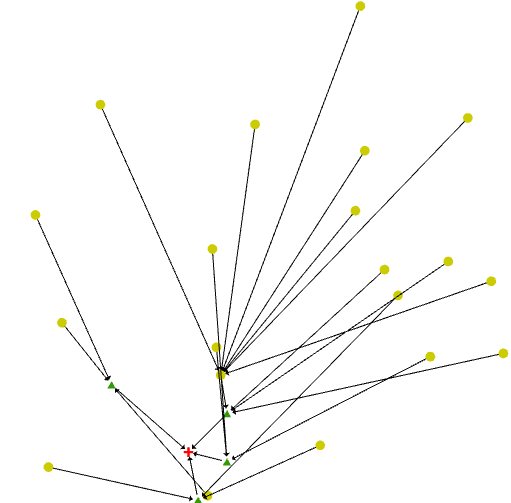
\includegraphics[width=0.70\textwidth]{Chap7/figures/khas_sim}
	\caption{MK-HK Simulation Example in RePast Simulator}
	\label{fig:sim}
	\end{figure}


%\begin{itemize}
%\item Network Builder
%\item Node
%	\begin{itemize}
%	\item Sensing
%	\item Routing
%	\item Central
%	\end{itemize}
%\item Darwin Core
%	\begin{itemize}
%	\item Identification
%	\item Location
%	\item Occurrence
%	\item Image
%	\item Species
%	\end{itemize}	 
%\end{itemize}

\subsection{Darwin Core}
The Darwin Core class represents a DwC archive, encapsulating \textit{Identification}, \textit{Location}, \textit{Occurrence}, \textit{Image} and \textit{Species} (Section \ref{buildcapture}). The images we have collected from Danau Girang were processed to find details such as the average size when captured at night and day, how often an average camera triggers and the percentage of images with animal content. These data were then used to specify how often a randomly placed node should capture an observation per tick.

Upon each capture, images are created and given a random size, between the maximum and minimum size found in the 120,000 images collected from DG. The sum of the image sizes is used to calculate the size of the archive. Using this size, a sensing node calculates how long the archive takes to send based on the size and the transmission rate. We assume that the rate stays constant for the duration of transmission.
When an archive is sent to the routing node, we used the average time for our image processing tool and Drools engine to run and attempt a classification, which is 43 seconds (ticks), explained in detail in Section \ref{tech:sf:triton}. To keep the classifications as general as possible, so that the simulation applies to any WSN for scientific observations, archives are not classified down to the species level, they are marked as \textit{interesting} or \textit{empty} and then forwarded to the central node.

\subsection{Routing}
The routing protocol used needs to be dynamic in order to adapt to nodes being added and removed during deployment, while minimising traffic in a resource constrained network. In our approach, we use a modification the Minimum Cost Forwarding Algorithm (MCFA), described in Section \ref{arch:routing}. A cost is assigned to each node, based on how far they are from the central node, with neighbouring nodes choosing to connect to the node with the lowest cost. However, in normal implementations of MCFA, all nodes are of the same type and simply need to connect to a base station. This protocol is used in all scenarios.

In our K-HAS architecture, sensing nodes cannot connect directly to a central node because processing would not take place. Because of this, we used the same routing method across all scenarios. Our implementation of MCFA works with a discovery phase and a transmission phase. The discovery phase is a scheduled event, taking place at the start of deployment but it can be run throughout deployment to react to nodes being added or removed. 

\subsubsection{Discovery}
	Discovery begins at each central node, scanning nodes in range for routing nodes and sending a broadcast packet, with a cost of 0, to inform them that they are within range of a central node. Links between Central and Routing nodes use W-Fi in all of our scenarios. Once received, routing nodes increment the count and forward the packet to any routing nodes within range of them, where we use the range of Zigbee. We found that this method overloaded the routing nodes and all sensing nodes within range would connect to the first routing node they receive the broadcast from. We then implemented a method, called \textit{load balancing} \cite{Gupta2003}, which uses the sensing nodes connected to a routing node to calculate whether it should offload new nodes to a neighbouring routing node.
	
	The maximum connections a routing node can have is determined by the total number of sensing nodes in the network divided by the total number of routing nodes, which is held in the knowledge base of the central node. Once a routing node has the maximum number of connections allowed, it starts to offload to a neighbouring routing node that is also in range of the sensing node requesting a connection. If there are no neighbouring nodes then the routing node exceeds the maximum number of connections allowed, to save sensing nodes being left with nowhere to send their data.
	
	If the sensing node that receives the broadcast does not have an existing route to a central node, or the cost of the current route is higher than the received route, it adds an edge to the routing node, increments the count and forwards it to all nodes in range. This process continues until the broadcast reaches the edge of the network. Nodes do not have global knowledge of the route to the central node, only of their neighbour with the lowest cost.
	
	This phase can be repeated throughout the course of the deployment, simply by scheduling it as an event to occur every \textit{n} ticks. However, the simulation currently only uses the discovery phase at the beginning of the deployment.
	
\subsubsection{Transmission}
	Once the discovery phase has been completed, providing nodes are within range of the central node, the transmission phase begins where only DwC archives are then sent across the network. Observations are captured based on the mode of the simulation and sent to the lowest cost neighbour.
	
	In order to manage transmissions, sensing nodes have a \textit{SendState} object that contains the next archive to send, the time to send it and whether it is currently sending. This is used to determine what operations to perform, once an archive has been sent, it is deleted from the SendState and the sending flag is set to false. A new archive is then added and sent when the opportunity arises.
	
	When a routing node receives the archive, it begins processing. Routing nodes use the SendState as well, but they only add an archive once it has been processed and they then select the oldest archive that has been classified as interesting, providing an archive is not already waiting to be sent. The archive stores information about the route it takes, recording every hop, as well as the time it took from capture to central node.
	
	Scheduled sending events run every thousand ticks, which is configurable, to check the sending state of the node and send any archives in the SendState. The node then waits for the number of ticks that it will take in order to transmit the archive.
	
	Once the simulation is completed, either manually or through a defined number of ticks, the archives in each central node are iterated over and written to a CSV file, with details such as the path it took, total transmission time and time of capture.
	
\subsection{Capture}
	Using the existing data collected from Danau Girang, we calculated how often a camera triggers in a six month deployment, as well as how often the observation contained interesting content. 
	
	To calculate the count of interesting images, we processed every directory of images to extract the largest object in the foreground, using our Triton program. Once processed, we iterated through every directory, counted the total number of images and the total number of extracted images. This gave us a 20.7\% chance of an image being interesting, across every camera.
	
	The chance of a camera being triggered each second was calculated by the total number of observations (13,399) divided by the number of seconds in six months (15,552,000). This gives a chance of 0.000861561 of a camera trigger in any given second.
	%Edit this to explain why it runs every 1000 ticks
	
\subsection{Processing}
	The types of knowledge processing capabilities that we outlined in Section \ref{sim:imp} are used in the simulation to determine which type of processing to perform on observations. The result of processing is that an observation is marked as interesting or empty. The limitation of our image processing tool is that only the largest region of interest (ROI) is extracted, even if there are multiple objects in the image. The outcome can be any of the following:
		\begin{description}
			\item True positive (TP): An ROI is extracted that contains the animal in the set.
			\item False positive (FN): An ROI is extracted that contains nothing of interest.
			\item True negative (TN): A camera is triggered with nothing of interest in the image and no ROI is extracted.
			\item False negative (FN): An image containing an animal has no ROI extracted.
		\end{description}
	
	Using the results of our image processing application (explained in Section \ref{tech:sf:triton}) for the properties of HK processing, we encoded that an 82\% accuracy at detecting TP images, with a 98\% accuracy for finding TN images. Nodes with MK do not have the ability to mark an image as empty, but they can mark an image as interesting. However, the results we have from our rule base are not as extensive as the results we have for Triton (due to limited local knowledge and existing rules approved by domain experts), so instead we use a predefined 10\% accuracy for detecting TPs. This 10\% is used because we needed to show the difference between a node with MK and a node with HK. HK nodes have the ability to process the contents and metadata of sensed data, with access to libraries and a dynamic knowledge base. MK nodes are able to look at the basic metadata and only have a static knowledge base, limited in size. In future work, we could test with greater accuracy or, with more rules, we could run experiments to find the exact accuracy of an MK node. An interesting image is an image that contains an animal and can be either a TP or FN. Empty images are those that do not contain an animal and can be either FP or TN.
	

\section{Results}\label{sim:res}
In this section, we explains the results from simulating each scenario in a randomly generated network graph. 

Each scenario, outlined in Section \ref{sim:imp}, runs to simulate a 6 month deployment. Using our motivating scenario, we modelled each scenario on a fixed number of nodes: 1 central node, 4 routing nodes and 20 sensing nodes. The implementation of our architecture has been limited to using Zigbee as the transmission medium between all sensing nodes, with a Wi-Fi connection between routing nodes and a central node. Sensing nodes then send an observation when it is captured or, if it has not captured anything then it checks for a backlog every ten minutes. Sensing nodes check for new observations to process every five minutes. We ran each scenario a hundred times, with each run simulating a 6 month duration. The time to process an observation using MK has been simulated to take 5 seconds compared to the 90 seconds when a node has HK capabilities; these values have been chosen based on the average processing time we derived using existing data. 

\begin{figure}[ht!]
	\centering
	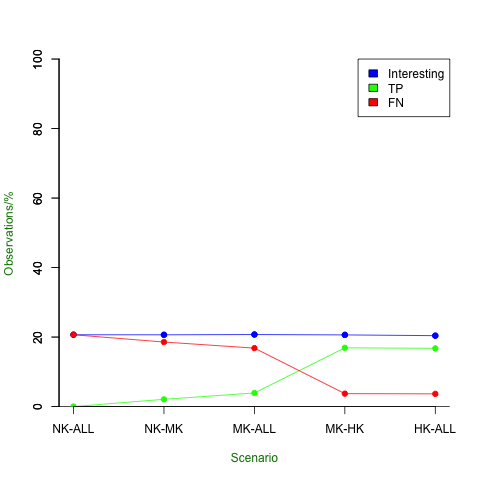
\includegraphics[width=0.7\textwidth]{Chap7/figures/ideal/all_int_percent}
	\caption{Percentage of Interesting Observations for All Scenarios.}
	\label{fig:res:ideal:int}
\end{figure}

The simulations were run in two modes: ideal transmission rate and variable transmission. Ideal used a fixed transmission rate (250kbps) for Zigbee links between all sensing nodes, with all observations being sent at the highest possible rate. Variable generates a random number for the transmission rate (between 20 and 250kbps) for each sensing node link, at the time of the network's initialisation. This models the large fluctuations in both speed and range that we observed in the Malaysian rainforest when we ran tests with Zigbee equipment. The Wi-Fi range remains constant because the distance of routing nodes from central nodes, in our motivating scenario, can be made small enough that a consistently good connection is achievable.

\begin{figure}[ht!]
\centering 
\begin{subfigure}{0.7\textwidth}
  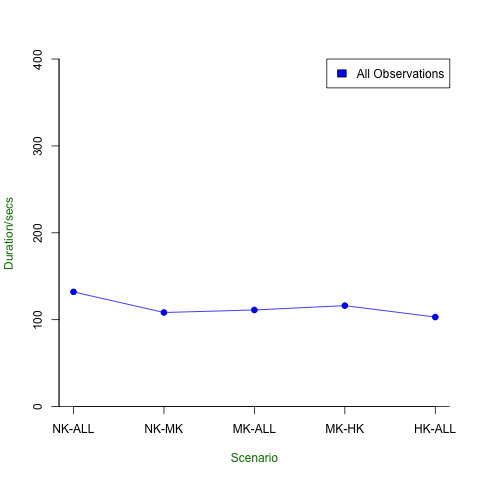
\includegraphics[width=0.8\textwidth]{Chap7/figures/ideal/all_total}
	\caption{Ideal Transmission Rates.}
	\label{fig:res:ideal:dur}
\end{subfigure}
\begin{subfigure}{0.7\textwidth}
  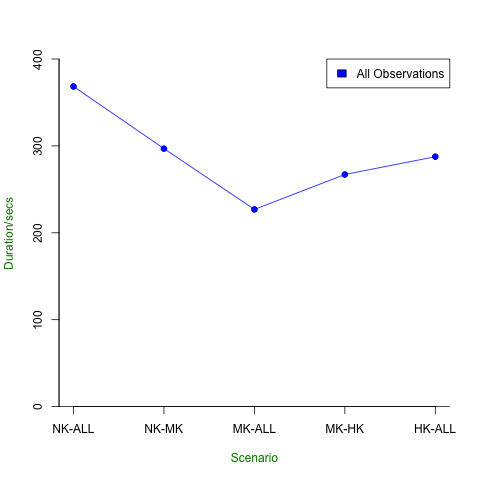
\includegraphics[width=0.8\textwidth]{Chap7/figures/real/all_total}
	\caption{Variable Transmission Rate.}
	\label{fig:real:dur}
\end{subfigure}
\caption{Mean Duration of All Observations}
\label{fig:mean:dur}
\end{figure}

Figure \ref{fig:res:ideal:int} shows the percentage of interesting observations that arrive at the central node. Due to the short transmission time, almost all observations arrive in near real-time (fewer than 2 minutes) and, as such, the split between empty and interesting remains almost constant at approximately 80:20. This is important because the chance of an image being interesting is 20.7\%, so all data is being received at the DA node, without any observations backed up on nodes in the network. However, the True Positive observations are the most important as they are the interesting observations that have been marked as such. False Positives are interesting observations that have been wrongly marked as empty. Increasing the knowledge processing capabilities of routing nodes, shown by the difference between MK-ALL and MK-HK, increases the number of TPs, as well as reducing the number of FPs. Another important point to note is that MK-HK and HK-ALL provide the same results, despite HK-ALL solely consisting of nodes with the highest knowledge processing capabilities.  This is probably due to the fact that all observations, in MK-HK, go through an HK routing node and, thus, would receive the same level of processing as in an HK-ALL scenario.

These results support our hypothesis that MK-HK is the best scenario to choose in terms of timeliness of data delivery, quality of data delivered and network lifetime, as MK-HK has all sensing nodes with minimal knowledge processing capabilities, allowing them to run for approximately three months, achieved from tests detailed in Section \ref{tech:hw:conc}. However, with HK-ALL, all sensing nodes run with higher capabilities and are limited to run for a maximum of three weeks before battery replacement is required. While this number is similar to the current, manual process described in Section \ref{tech:motiv}, this does include processing and prioritisation of sensed data, which can take weeks or, sometimes, months when carried out by humans.

\subsection{Duration}
The ideal transmission rate runs with the transmission rates of all nodes at their theoretical maximum, giving the highest speed for both Zigbee and Wi-Fi. Figure \ref{fig:res:ideal:dur} shows the mean duration of any observation, interesting or empty, in each scenario. With the exception of NK-ALL, it is clear scenarios that, where more nodes have higher knowledge processing capabilities, the mean duration is increased. An explanation for NK-ALL nodes showing a higher average duration is because the lack of knowledge on any of the nodes prevents it from prioritising observations, which means that some could be queued for longer before being sent on. One of the key points to note is that the difference in transmission time from capture to central node is typically no more than one hundred seconds. When compared with a standard, power efficient WSN with no knowledge processing capabilities, the reduced battery life may not be worth the trade off. However, these times are not solely for transmission, they also include in-network processing and prioritisation when they arrive at the central node. 

\begin{table}[h]
\centering
\begin{tabular}{|l|l|l|l|l|l|}
\hline 
      & Total & Interesting & \% Interesting & Empty & \% Empty \\
\hline
NK-ALL & 44205 & 9133        & 20.7           & 35071 & 79.3     \\
NK-MK  & 44244 & 9136        & 20.6           & 35107 & 79.4     \\
MK-ALL & 44052 & 9132        & 20.7           & 34920 & 79.3     \\
MK-HK  & 43754 & 10066       & 23.0           & 33688 & 77.0     \\
HKALL & 42511 & 9671        & 22.7           & 32840 & 18.9     \\
\hline   
\end{tabular}
\caption{Mean Number of Observations for All Scenarios under Ideal Transmission Rate}
\label{sim:tab:ideal}
\end{table}

During our visits to Danau Girang, we performed experiments for many different transmission methods: Wi-Fi, Zigbee and RF. The results were always different to what we experienced in the UK and the variation in connectivity in just a few minutes, or metres, was extreme in some cases. Days where the humidity was one percent higher than the previous day could result in a 50\% range drop and rain for a few minutes could drop all connections for an hour afterwards. Modelling this in our simulations was necessary to accurately plan for what we could expect in Malaysia. Our planned network topology (Section \ref{arch:scen}) in Danau Girang has routing and central nodes so close to each other that the Wi-Fi connection remained fairly stable and connectivity should remain at 100\%. When simulating sensing nodes, we randomly set their transmission rate between 20 and 250kbps at the start of each run. As each scenario is being run 100 times, this method is more efficient while still allowing for variation in the transmission rates. 

The number of interesting observations received in each scenario remained similar to the ideal mode (see Tables \ref{sim:tab:ideal} and \ref{sim:tab:variable}), as expected, but the fluctuation in transmission time (Figure \ref{fig:real:dur}) is much larger, with some images taking 800 seconds, or 13 minutes. In our motivating scenario, this is not much of an issue. However, if the image was of a hunter or the scenario was building intrusion detection system, then thirteen minutes is a long delay that could cause considerable damage. Of course, using all Wi-Fi connections is a more feasible option, but situations where long range is required prevents this and these simulations do not currently take into account broken links in the network, where changes to the node's environment (such as a fallen tree) that could block its signal or an increase in humidity, could cause it to drop out of range for minutes or even hours. 

The duration of an observation with both a variable and ideal transmission rate does not fluctuate largely and Figure \ref{fig:res:ideal:int} shows that the processing power of MK-HK vs. HK-ALL is identical. However, Figures \ref{fig:real:int:dur} and \ref{fig:real:empty:dur} show that the primary benefit of pushing HK processing capabilities out to the edge of the network allows for better prioritisation of observations. Sensing nodes with HK are able to determine whether an observation is interesting or empty with much greater accuracy than MK and these capabilities, right at the edge of the network, allows for an interesting observation to be processed as soon as it is captured and sent without further processing directly to a central node. The only delays being the processing time itself and the sending queue of intermediate nodes. Figures \ref{fig:real:int:dur} and \ref{fig:real:empty:dur} show that, when a network is not saturated, interesting and empty observations take a similar amount of time to pass through the network; with the exception of the HK-ALL scenario. WSNs with much worse transmission rates could experience a much larger time difference between interesting observations, especially when using long range FM frequencies that can transfer only a few bytes a second.
\begin{figure}[ht!]
\centering
    \begin{subfigure}{0.7\textwidth}
	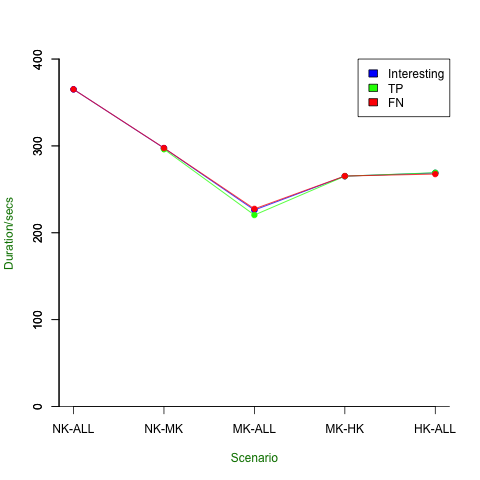
\includegraphics[width=0.8\textwidth]{Chap7/figures/real/all_int}
	\caption{Interesting Observations.}
	\label{fig:real:int:dur}
	\end{subfigure}	

	\begin{subfigure}{0.7\textwidth}
	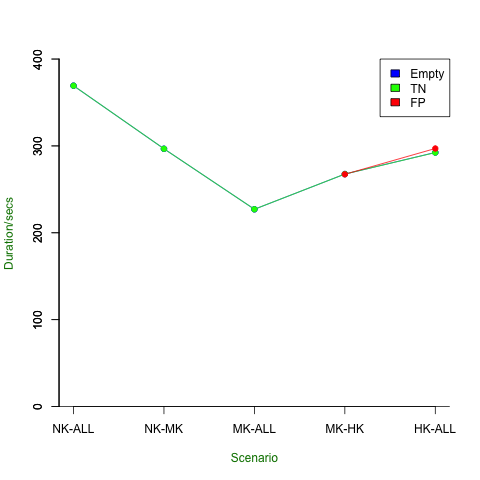
\includegraphics[width=0.8\textwidth]{Chap7/figures/real/all_empty}
	\caption{Empty Observations.}
	\label{fig:real:empty:dur}
	\end{subfigure}	
\caption{Mean Duration under Variable Transmission Rate}
\end{figure}

\begin{table}[h]
\centering
\begin{tabular}{|l|l|l|l|l|l|}
\hline
      & Total & Interesting & \% Interesting & Empty & \% Empty \\
\hline
NK-ALL & 43743 & 9012        & 20.6           & 34730 & 79.4     \\
NK-MK  & 44258 & 9195        & 20.8           & 35063 & 79.2     \\
MK-ALL & 44152 & 9130        & 20.7           & 35021 & 79.3     \\
MK-HK  & 44273 & 10183       & 23.0           & 34059 & 77.0     \\
HKALL & 43011 & 9935        & 23.1           & 33076 & 18.9     \\
\hline
\end{tabular}
\caption{Mean Number of Observations for All Scenarios under Variable Transmission Rate}
\label{sim:tab:variable}
\end{table}

\subsection{Network Saturation}



With the transmission rates of Zigbee and Wi-Fi, an observation of three images, each under a megabyte in size, can be processed and sent in a matter of minutes; when there are only a few hops. However, with these network topologies, we are unable to see how each scenario handles prioritisation when it is unable to send every observation captured. This can be done by either reducing the transmission rate or increasing the chance of an observation being captured. We chose to increase the chance of an observation being captured and maintaining the transmission rate in order to keep the simulations in line with our motivating scenario. Existing data from Danau Girang has shown a seasonality change in the number of images captured and we know that some sites are more active than others, therefore making a higher chance of capture more fitting. 

Imagine a scenario where flash floods in the rainforest prevent access to the nodes to change the battery and a mating season of sun bear has caused the capture rate to increase. The chance of an image capture has increased and users of the network have programmed the sensing nodes's sleep duration to a minute; saturating the network with more images than can be sent in a six month period.

\begin{table}[h]
\centering
\begin{tabular}{|l|l|l|l|l|l|}
\hline
      & Total  & Interesting & \% Interesting & Empty  & \% Empty \\
\hline
NKALL & 254352 & 127149      & 50           & 127149 & 50     \\
NKMK  & 264580 & 144058      & 54.4         & 120522 & 45.6     \\
MKALL & 183727 & 126530      & 68.9           & 57196  & 31.1     \\
KHAS  & 159446 & 115054      & 72.2           & 44392  & 27.8     \\
HKALL & 192010 & 155656      & 81             & 36353  & 18.9     \\
\hline
\end{tabular}
\caption{Mean Number of Observations for All Scenarios when Saturated}
\label{sim:tab:satur}
\end{table}

We simulated this across all five scenarios and the results are detailed in this section. The duration is increased for all observations (Figure \ref{fig:sat:total:dur}) and there is an increase in the time it takes an interesting observations when compared to an empty observation. Table \ref{sim:tab:satur} shows the average number of observation captured across all scenarios, however, when you look at the number delivered, we can see that the number of interesting observations delivered is much greater. This means that the network is successfully prioritising observations it believes to be interesting and not sending those that are empty because of the time and bandwidth constraints.

	\begin{figure}[ht!]
	\centering
	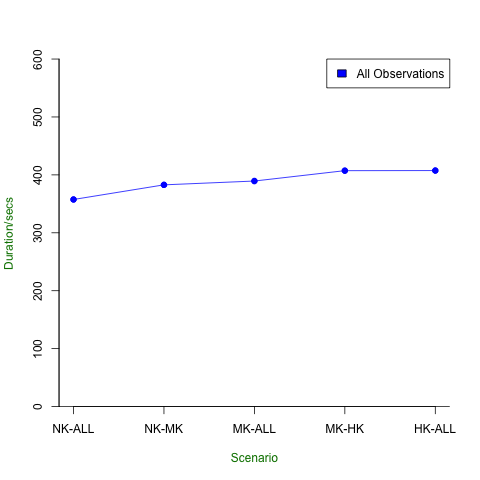
\includegraphics[width=0.7\textwidth]{Chap7/figures/saturated/all_total}
	\caption{Mean Duration of All Observations Across All Scenarios}
	\label{fig:sat:total:dur}
	\end{figure}

Figure \ref{fig:sat:total:dur} shows that the mean transmission time of all observation does not differ much between scenarios (with all scenarios at approximately 400 seconds) when the network is saturated, but we can see that the network must decide what images to send or drop when there are more observations than bandwidth available. HK-ALL is the slowest of these because of the increased time it takes to process and image with HK. This is shown more clearly when we compare \textit{interesting} and \textit{empty} observations. The red line (showing false positives) only exists for MK-HK and HK-ALL scenarios because MK nodes are not able to classify an observation as empty and, as such, NK-ALL, NK-MK and MK-ALL do not generate any false positives.

	\begin{figure}[ht!]
	\centering
		\begin{subfigure}{0.7\textwidth}
		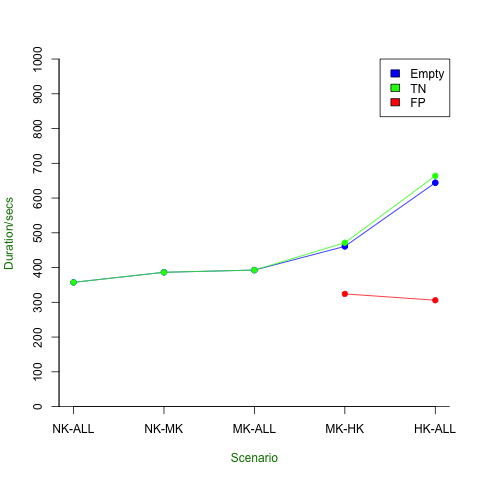
\includegraphics[width=0.8\textwidth]{Chap7/figures/saturated/all_empty}
		\caption{Empty.}
		\label{fig:sat:empty:dur}
		\end{subfigure}

		\begin{subfigure}{0.7\textwidth}
		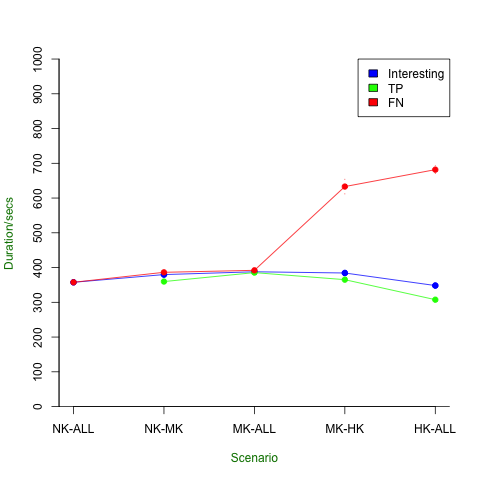
\includegraphics[width=0.8\textwidth]{Chap7/figures/saturated/all_int}
		\caption{Interesting.}
		\label{fig:sat:int:dur}
		\end{subfigure}
	\caption{Mean Duration of Observations across All Scenarios}
	\end{figure}

The mean transmission time of empty images (Figure \ref{fig:sat:empty:dur}) shows that the increase of knowledge processing capabilities improves the network's ability to filter out empty observations and a network with only HK nodes is able to defer empty observations from the time of capture so that bandwidth remains free for those that are interesting. Figure \ref{fig:sat:int:dur} shows the mean transmission time of interesting observations and we can see that interesting observations misclassified as empty bring the average duration for interesting observations up to approximately 400 seconds but the ability to prioritise allows TP observations to be delivered at a much faster rate of between 300 and 400 seconds, compared to more than 800 seconds for empty observations. It is worth nothing that, while misclassified interesting observations (FP) take longer to reach the central node in higher knowledge scenarios, the number of them received is greatly reduced from between 30\% and 45\% in MK scenarios to less than 20\% for HK scenarios; as shown in Figure \ref{fig:sat:int:percent}.

	\begin{figure}[ht!]
	\centering
	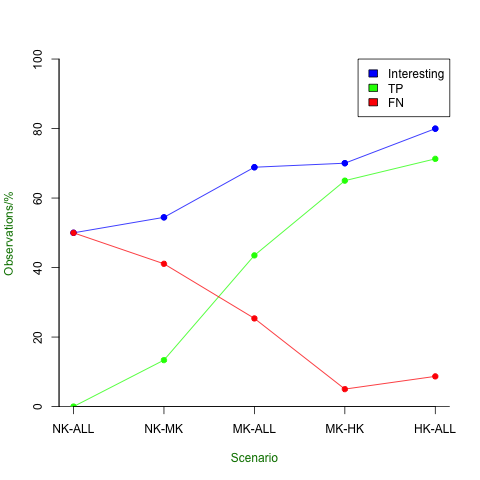
\includegraphics[width=0.7\textwidth]{Chap7/figures/saturated/all_int_percent}
	\caption{Percentage of Interesting Observations across All Scenarios}
	\label{fig:sat:int:percent}
	\end{figure}

	\begin{figure}[ht!]
	\centering
	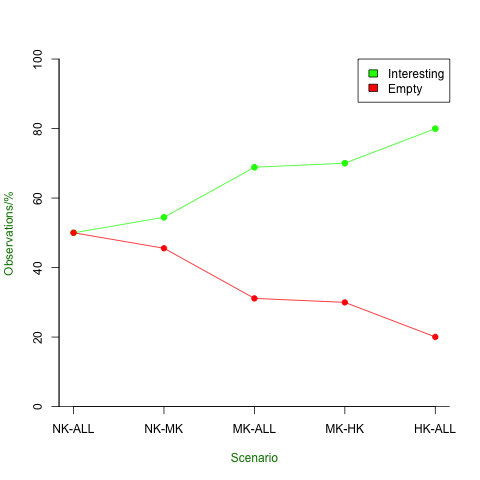
\includegraphics[width=0.7\textwidth]{Chap7/figures/saturated/all_int_empt}
	\caption{Percentage of Interesting Compared to Empty Observations across All Scenarios}
	\label{fig:sat:int:empty}
	\end{figure}

Saturating each scenario shows how different levels of knowledge processing across the the nodes can prioritise the delivery of interesting observations while filtering out observations that have been classified as empty. We can see that the HK-ALL scenario delivers the highest percentage of interesting observations (80\%), with a slightly higher average transmission time. Having HK on all nodes causes a large reduction in the lifetime of the network to 3 weeks. L-KHK (or KHAS) is a good alternative to this as it provides a network lifetime of 3 months for the majority of the nodes but still around 70\% of all images (same as MK-ALL) are interesting, but the majority of these are \textit{true positives}. In a network with limited access to a power source, MK-HK is the best implementation but, for networks with access to a continuous power source, HK-ALL can be used to increase the number of interesting observations delivered to the central node in a shorter time period.

% \subsection{Scenarios}

% This section details the results from each scenario of increasingly capable knowledge processing nodes. NK-ALL represents a 'standard' WSN where no nodes have knowledge processing capabilities and forward to a single endpoint. NK-MK simulates a network where sensing nodes have no knowledge processing capabilities, but routing nodes have MK, allowing them to detect whether an observation is interesting, but lack the knowledge to determine, with any confidence, whether an observation is of no interest. MK-ALL simulates a network where both sensing and routing nodes have MK capabilities. MK-HK is the RePast implementation of our K-HAS architecture; sensing nodes have MK and routing nodes have HK. HK-ALL has sensing and routing nodes that have HK capabilities. 

% Table \ref{tab:observ_int} shows the time for average transmission time, in hours, for interesting observations. Interesting observations consist of \textit{true positives} and \textit{false negatives}, which means that the spread of transmission times would be quite varied, because TPs would be prioritised but FPs would be treated as empty images. However, we can see that the total of interesting images almost doubles when all nodes have HK. More importantly, the difference between HK-ALL and MK-HK is less than 2\%, while still providing a battery advantage. With MK-HK and HK-ALL, the median is much lower when compared to MK-ALL and NK-MK, due to the higher levels of knowledge processing capabilities.

% With the results broken down further, Table \ref{tab:observ_tp} shows the average duration for true positives and we can see that, while the median stays much the same for each scenario, average duration varies considerably. The average time for a TP to be sent is lower for MK-HK than for MK-ALL, this could be due to the extra processing time for HK nodes or a processing backlog with a large number of observations. Although the duration of MK-HK is approximately twice that of MK-ALL, it does deliver more TPs, with 36.46\% of all images received being TP, compared with 8.45\% for MK-ALL.

% \begin{table}[h]\footnotesize
% \begin{tabularx}{\textwidth}{ |X|X|X|X|X|}
% \hline
% Scenario & Median & Mean & Standard Deviation & \% Total\\
% \hline
% NKMK & 608 & 841.95 & 854.18 & 22.11\\
% MKALL & 127 & 652.33 & 868.09 & 24.35\\
% MKHK & 3 & 255.49 & 591.63 & 38.86\\
% HKALL & 2 & 59.57 & 320.48 & 40.78\\
% \hline
% \end{tabularx}
% \caption{Transmission Time for Interesting Observations}\label{tab:observ_int}
% \end{table}

% \begin{table}[h]\footnotesize
% \begin{tabularx}{\textwidth}{ |X|X|X|X|X|}
% \hline
% Scenario & Median & Mean & Standard Deviation & \% Total\\
% \hline
% NK-MK & 3 & 277.01 & 543.22 & 3.88\\
% MK-ALL & 2 & 99.73 & 353.16 & 8.45\\
% MK-HK & 3 & 207.09 & 518.11 & 36.46\\
% HK-ALL & 2 & 2.77 & 2.75 & 38.16\\
% \hline
% \end{tabularx}
% \caption{Transmission Time for True Positive Observations}\label{tab:observ_tp}
% \end{table}

% \begin{table}[h]\footnotesize
% \begin{tabularx}{\textwidth}{ |X|X|X|X|X|}
% \hline
% Scenario & Median & Mean & Standard Deviation & \% Total\\
% \hline
% MK-ALL & 675.5 & 945.94 & 916.11 & 15.9\\ 
% MK-HK & 683 & 989.02 & 1006.4 & 2.41\\
% HK-ALL & 553 & 885.65 & 931.19 & 2.6\\
% \hline
% \end{tabularx}
% \caption{Transmission Time for False Negative Observations}\label{tab:observ_fn}
% \end{table}

% \begin{figure}[!h]
% \centering
% 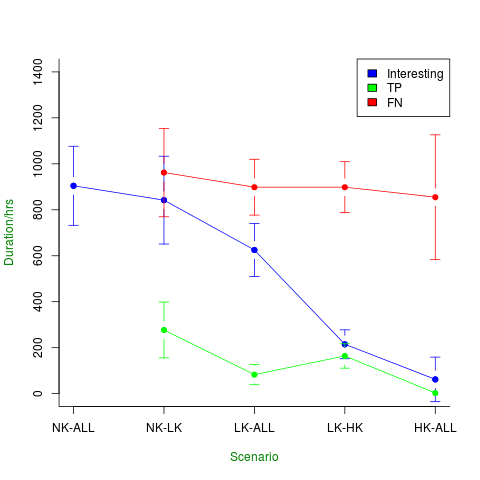
\includegraphics[width=\textwidth]{Chap7/figures/all_int.png}
% \caption{Mean Transmission Time for Interesting Observations in All Scenarios}
% \label{fig:all_int}
% \end{figure}

% \begin{figure}[!h]
% \centering
% 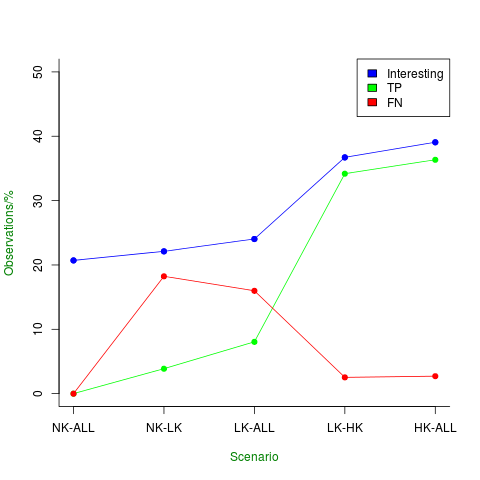
\includegraphics[width=\textwidth]{Chap7/figures/all_int_percent.png}
% \caption{Percentage of Interesting Observations in All Scenarios}
% \label{fig:all_int_percent}
% \end{figure}

% Figure \ref{fig:all_int} shows the average transmission time for interesting observations across every scenario. NK-ALL has no points for TP and FN because of its lack of processing capabilities. The drop in transmission time for interesting images is clearly visible here, but there is an increase in TN transmission time when comparing MK-ALL and MK-HK. This spike is better explained with the use of Figure \ref{fig:all_int_percent}, showing that, although it takes longer for TP images to be delivered in MK-HK, the percentage of TP images increased in MK-HK by almost four times that of MK-ALL. The faster transmission times in HK-ALL can be explained by the fact that all nodes can accurately detect empty images from the edge of the network and also prioritise interesting images with a greater accuracy than any other scenario. However, nodes with HK processing power have much higher power requirements and require battery changes every 3 weeks, this power trade off shows that nodes of this type can deliver interesting observations significantly faster than nodes with MK. A number of WSNs will place nodes in places that are not easily accessible by humans and not expected to be visited so regularly. In our motivating scenario, some nodes could be rendered inaccessible by river floods for weeks at a time and regular human traffic can prevent animals from using those sites. The percentage of TPs delivered by MK-HK and HK-ALL are not that different, but the delivery time when using both HK and MK nodes does affect the delivery time. 

% \subsection{MK-HK Scenarios}

% The main difference between HK-ALL and MK-HK is that all sensing nodes in HK-ALL have the ability to perform more intense data processing and determine which observations to prioritise with greater accuracy. Whereas MK-HK focusses on HK capabilities for the routing nodes and maximising the lifetime of sensing nodes by limiting them to MK capabilities. Therefore, we tested different proportions of MK and HK sensing nodes within the MK-HK scenario in order to determine the best ratio between performance and network lifetime. Table \ref{tab:khas_int} shows the average duration for an interesting observation when 4, 8, 12, 16 and 20 of the 20 sensing nodes have HK, with the rest having MK processing capabilities. Figure \ref{fig:khas_int_percent} illustrates how pushing knowledge further towards the edge of the network increases the delivery time and the percentage of interesting images. MK-HK 16 and MK-HK 20 have an average difference of three hours for interesting images, but MK-H K20 means that all nodes in the network have HK processing capabilities and, thus, a shorter battery life. While the difference in transmission time is not that significant, the extra MK nodes with a longer battery life means that they can be placed in areas that may not be easily accessible or need to remain undisturbed.

% \begin{table}[h]\footnotesize
% \begin{tabularx}{\textwidth}{ |X|X|X|X|}
% \hline
% Scenario & Median & Mean & Standard Deviation \\
% \hline
% MK-HK 4 & 2 & 153.21 & 462.75 \\
% MK-HK 8 & 2 & 146.04 & 428.79 \\
% MK-HK 12 & 2 & 156.95 & 461.67 \\
% MK-HK16 & 2 & 88.86 & 349.68 \\
% MK-HK 20 & 2 & 63.13 & 330.67 \\
% \hline
% \end{tabularx}
% \caption{Transmission Time Results for Interesting Observations}\label{tab:khas_int}
% \end{table}

% \begin{table}[h]\footnotesize
% \begin{tabularx}{\textwidth}{ |X|X|X|X|}
% \hline
% Scenario & Median & Mean & Standard Deviation \\
% \hline
% MK-HK 4 & 2 & 104.74 & 393.06 \\
% MK-HK 8 & 2 & 94.56 & 357.04 \\
% MK-HK 12 & 2 & 86.85 & 343.69 \\
% MK-HK16 & 2 & 29.15 & 191.82 \\
% MK-HK 20 & 2 & 2.08 & 1.93 \\
% \hline
% \end{tabularx}
% \caption{Transmission Time Results for True Positive Observations}\label{tab:khas_tp}
% \end{table}

% \begin{figure}[!h]
% \centering
% 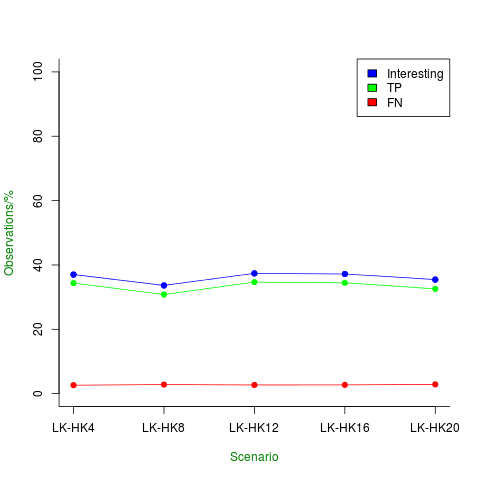
\includegraphics[width=\textwidth]{Chap7/figures/khas_int_percent.png}
% \caption{Percentage of Interesting Observations in MK-HK Variations}
% \label{fig:khas_int_percent}
% \end{figure}

% \begin{figure}[!h]
% \centering
% 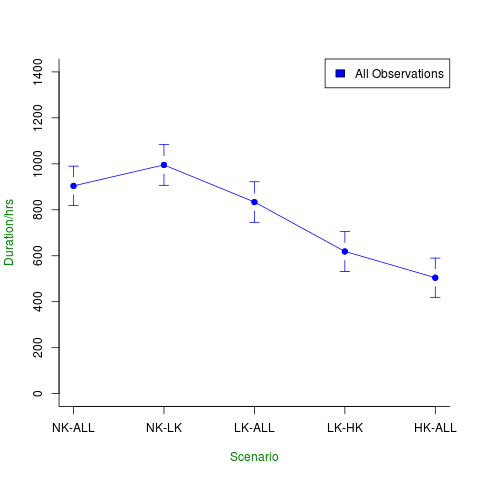
\includegraphics[width=\textwidth]{Chap7/figures/all_total.png}
% \caption{Mean Duration for All Observations in Zigbee Scenarios}
% \label{fig:all_total}
% \end{figure}

% \subsection{Unrestricted Transmission Speeds}
% In this section, we manipulated the variables set in out original simulations, that were based on existing sensed data, to identify bottlenecks that prevented observations from being received immediately. Zigbee has a low transmission rate, of 2.77 Kbps, therefore we expected increasing the transmission rate of all nodes in the network to a rate in the thousands (61920 Kbps) to determine whether this would reduce the mean transmission time for all images. Figure \ref{fig:unres_int} shows that, when compared with Figure \ref{fig:all_int}, the transmission time is reduced in all scenarios, by up to half in some cases. HK-ALL shows that this increase allows for interesting observations to be delivered with almost no delay, in near real-time. However, with a rate that should allow almost all observations to be sent in a matter of seconds, many scenarios still have a delay of 600 hours. Figure \ref{fig:unres_total} shows the average duration for all observations received at the central node and, with Wi-Fi transmission rates, we expected this to be much higher. However, when compared with Figure \ref{fig:all_total}, which shows the average duration for all observations using Zigbee as the transmission medium, we can see that the transmission time for most scenarios reduces to fewer than 500 hours. HK-ALL, remains much the same, despite the faster transmission rate. 

% Another bottleneck that we identified was the duration that each node would check for new observations, and process them. In the current solution, sensing nodes check every 10 minutes and routing nodes check every 5. This delay could cause an observation to not be picked up immediately, as well as the transmission delay. To test this, we reduced the Sensing node check to every minute and the Routing node to check every 30 seconds for new observations. Using Zigbee, the mean transmission time for all observations, in the HK-ALL scenario, was 501.02 hours. Using the increased transmission rate, it was 354.34 hours and with the reduced checking delay, the time dropped to 1.58 hours. Therefore, in order to create a real time implementation of these scenarios, one would need to use a fast transmission medium, such as Wi-Fi, and increase the time delay to check for new data; both of which would reduce the battery life of the node. This solution would ensure that all sensed data would be received almost as soon as it was captured, however, our HK-ALL Zigbee implementation would deliver interesting images within 3 hours but conserve battery life by using a radio with less power consumption and checking for new data less often. This faster solution would be primarily suited to deployments where power is not a constraint, but the real-time receipt of all sensed data is.

% \begin{figure}[!h]
% \centering
% 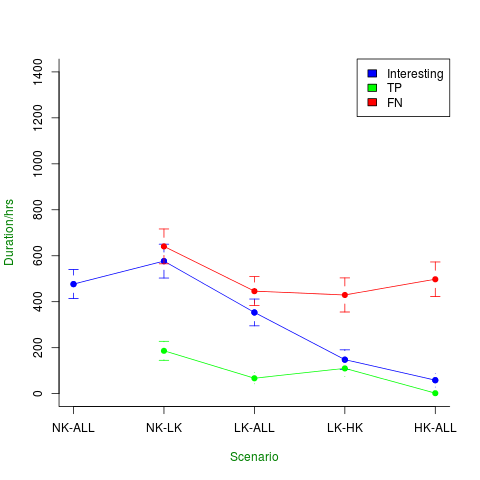
\includegraphics[width=\textwidth]{Chap7/figures/unres_all_int.png}
% \caption{Mean Duration for Interesting Observations in Unrestricted Scenarios}
% \label{fig:unres_int}
% \end{figure}

% \begin{figure}[!h]
% \centering
% 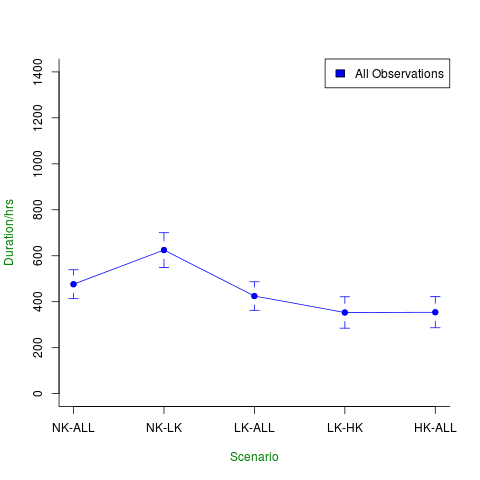
\includegraphics[width=\textwidth]{Chap7/figures/unres_all_total.png}
% \caption{Mean Duration for All Observations in Unrestricted Scenarios}
% \label{fig:unres_total}
% \end{figure}

\section{Conclusion} \label{sim:conc}
	
In this chapter, we have detailed the development of simulations to show the different scenarios for pushing knowledge out to the edge of a network. Using different levels of knowledge processing capabilities on nodes, we have shown that a network with HK processing capabilities can detect and prioritise interesting images, while simultaneously delaying empty images for a time when the network is not busy. However, using a network that solely comprises of HK nodes results in a battery life that lasts for 3 weeks on each node. The MK-HK network architecture we have proposed provides a combination of HK and MK nodes, distributed based on their role in the network. For example, nodes tasked with sensing and forwarding images only have MK processing capabilities. These simulations have shown that the HK-MK scenario results in a delay of interesting image delivery, when compared to MK-ALL, but the percentage of interesting images delivered is significantly increased.

Using a model of real world transmission rates, we have seen that the variation in transmission times can be quite large, but the difference between MK-HK and HK-ALL is not that great. This suggests that our MK-HK proposal (K-HAS) is the best solution for most scenarios as it provides a longer network lifetime with same ratio of TP:FN images as a network where every node is equipped with HK.

While the simulation is not feature complete, it is accurate enough to show how MK-HK utilises the knowledge-processing capabilities at each tier to process, and prioritise, sensed data based on knowledge gained from the environment, previously sensed data and from humans using the network. Our results also show that the difference between MK-HK and HK-ALL is  not significant enough to warrant the loss in network lifetime. However, not every scenario would be suited to this. NK-MK shows a slightly faster transmission time and a much longer network lifetime, as most nodes would not have any processing power. While the processing of sensed data would not be enough to rely on, it could act as pre-processing that could be processed further once power is not an issue. This would be well suited for networks where nodes have limited power and are not easily accessible, such as bird nest monitoring networks. 

MK-HK allows sensed data to be processed, and delivered, in near real-time with approximately 87\% of all interesting data being correctly classified. This number could increase the longer that the network is deployed, which is something we would like to investigate in the future.

Finally, we simulated the situation where there is more sensed data than the bandwidth available. The greater knowledge-processing capabilities of HK-ALL scenarios ensured that empty images were delayed and interesting observations were sent with a greater priority. While there were interesting observations misclassified as empty that were delayed, they made up less than 10\% of all interesting observations. MK-HK did receive fewer interesting observations, most likely due to its limited ability to prioritise sensed data right from the edge of the network, but the majority of interesting observations were true positives and they were prioritised over empty observations. MK-ALL, with a longer network lifetime of MK-HK and HK-ALL, did not prioritise interesting over empty data effectively but still provided more true positives than false negatives.

We can conclude that, for a power efficient WSN, the results from these simulations suggest that MK-HK can deliver many of the same benefits that HK-ALL provides while not pushing HK to the edge of the network, reducing the network lifetime. If power was of no concern, HK-ALL is able to deliver more interesting observations and prioritise more accurately from the edge of the network, as well as filtering important data more effectively when the network is saturated.









































\chapter{Conclusion and Future Work}
In this thesis, we aimed to show that utilising the local knowledge of an environment in a WSN improves the efficiency of the network by giving it the ability to prioritise sensed data based on the results of in-network processing.  We believe that pushing knowledge out farther towards the edges of the network improves the overall performance. To show this, we have developed a three-tier WSN architecture that uses knowledge-processing capabilities to process sensed data as it is forwarded through the network. Most current WSN implementations deliver data chronologically, or store it on the node to be retrieved by queries. We believe that this knowledge can be used to infer how valuable sensed data is and prioritise that through the network, delivering the most interesting data first. However, resources are still limited in WSNs and our architecture had to utilise these resources effectively, such as battery life and bandwidth, to maximise the network lifetime. Using Data Collection (DC) nodes at the edge of the network, they capture observations and use their limited knowledge-processing capabilities to enrich the sensed data before sending it on. Data Processing (DP) nodes use more powerful knowledge-processing features to attempt to classify observations and prioritise the sending of them to Data Aggregation (DA) nodes. DA node make the data available to users and use their classifications, and input, to dynamically update its knowledge base.

We used a collaboration with a research centre in Malaysia with the aim to implement K-HAS in the Malaysian rainforest, in an area that had experienced logging and contained a diverse range of rare wildlife. Using K-HAS, we wanted to deploy a network that would prioritise images of rare wildlife and only send images of common wildlife when bandwidth was available.  Over the course of 3 visits, we gathered knowledge from the area, researchers and locals to build a knowledge base and create rules that could be used to classify data. We also collected images taken from their current, manual solution to infer patterns and use existing classifications for new sensed data.

Current sensing technology means that K-HAS is not ready to be implemented as the architecture dictates. DC nodes are not yet readily available, and this is especially true for image capturing sensor nodes. Because of this, we modified the architecture to use commercial hardware with fewer capabilities that would allow us to actually deploy a sensor network in the Malaysian rainforest that does use local knowledge. We call this architecture LORIS, Local-knowledge Ontology-based Remote-Sensing Informatics System, and this solution combines the DA and DP node to hold all of the knowledge-processing capabilities.

LORIS has shown that even using local knowledge at the base station of a WSN means that sensed data is processed and organised within minutes of being received. This method also means that users are alerted to data that they have subscribed automatically.

Our simulations of K-HAS show that the bandwidth in a WSN is used more effectively when knowledge is pushed out towards the edge of the network, allowing nodes to perform knowledge-processing to make inferences about the contents of the data and prioritise, or delay, its delivery appropriately. We have no reason to think that this would not work in practice.


\section{Summary of Contributions}
In this section, we summarise the contributions detailed in this thesis, focussing on our deployment in Malaysia, the tiered architecture designed for general use and the alignment ontology created to formalise the architecture of K-HAS and the data standard that it uses. 
\subsection{K-HAS}
In Chapter 4, we present a novel tiered architecture, K-HAS, for WSNs that uses local knowledge. We explored existing networks, those related to our motivating scenario in Malaysia and also those that use knowledge or context-awareness, and routing protocols that use the sensed data to determine how it is routed. We explain the purpose of each tier in the network and show how sensed data is enriched and routed as it progresses through the network. Using Darwin Core as a data standard, each node communicates in a common format and metadata is packaged with data in archives that can be read by any node in the network. We also show how rules can be used to infer the content of sensed data and the ability to run rule engines in the network allows sensed data to be prioritised based on its value; not just the time it was captured.
\subsection{Ontology}
In Chapter 5 we explain the aligning ontology created to formally represent the K-HAS architecture and the data standard used. We show how, while there are existing ontologies that join observation-centric and sensor-centric ontologies, K-HAS allows for the representation of knowledge exchange in the network and show nodes performing tasks similar to humans.
We also show how the ontology is extensible and does not need to be specific to K-HAS; it can be used with any WSN that deals with scientific observations. 
\subsection{LORIS}
In Chapter 6, we present the Local-knowledge Ontology-based Remote-Sensing Informatics System (LORIS), a system developed for our motivating scenario when we discovered that current sensing technology means that K-HAS is not ready to be implemented in its current form. DC nodes are not a type of sensor that is readily available, and this is especially true for image capturing sensor nodes. Because of this, we modified the architecture to use commercial hardware with fewer capabilities that would allow us to deploy a sensor network in the Malaysian rainforest that does use local knowledge. This solution combines the DA and DP node to hold all of the knowledge-processing capabilities and then uses commercially available sensors to replace DC nodes. 

This architecture is easier to implement but does not provide in-network processing, although it automates the delivery of sensed data and uses the increased knowledge-processing capabilities of modern PCs to process sensed data on arrival and inform users. We show how our deployment of LORIS was successful and highlighted how sensed data was delivered within minutes of being captured in some cases, and processed shortly after. 
\subsection{Simulations}
In Chapter 7, we explain the implementation and results of our simulations to model an ideal deployment of K-HAS. We model every variable of the network on existing data collected from our motivating scenario and show that the delivery of observations can be reduced by more than four hundred hours, when compared to the current manual solution. We also outline how the network is able to prioritise data that it believes to be interesting, using a priority queue mechanism that delays data it believes to be empty. Comparing K-HAS to different network implementations, where nodes have different levels of knowledge processing capabilities, shows that our network implementation is more power efficient than a network where every node has higher knowledge processing capabilities, yet its performance is similar.

\section{Future Work}
The focus of this thesis is to show that local knowledge can improve the timeliness of interesting data by making inferences based on previously sensed data and knowledge of the environment. We have shown, using simulations, that this can be done with our tiered approach. However, another aim was to deploy such an architecture for our collaborators. We have explained that current technology means that this is not feasible, but sensing, and microcomputer technology has moved forward significantly since the beginning of this PhD and it would be possible with a longer time period. Our deployment in Malaysia was limited due to time constraints and we would haved liked to leave a functional deployment active in Danau Girang for a six month period. 

With more time, we could create custom DC nodes using webcams and micro-computers, like the Raspberry Pi, encased in a watertight enclosure; allowing us to use higher levels of knowledge-processing at the edge of the network. A deployment of this length would also allow nodes to act on sensed data classified by users and update their knowledge base, responding to changes in the network dynamically.

K-HAS uses a combination of open source projects and some software created during the course of this work, but it does require specialist knowledge to be deployed. We would like to create an installation candidate that would be usable by those without any expertise that could provide basic information on the purpose of the network and the installation of all necessary packages would be automated.

On top of this, our software's user interfaces have been tested by researchers at Danau Girang but we have no metrics on the usability of the software. Testing the software on users to determine how they would score the different areas of the software, such as usability, response time and learning curve, would help us to improve the software and ensure that it can be used by those without any technical knowledge of K-HAS or its underlying architecture.

Experiments have shown us that the range of wireless transmissions is often hard to predict and can be heavily influenced by weather and obstacles. If sensors were placed at the edge of range for a neighbouring sensor, then it is not guaranteed that transmissions could be made every time. We believe that using humans as an intermediate hop could be an interesting research opportunity. Using a mobile app to transfer data between nodes as they are within walking range could speed up data transfers and their knowledge could be used to prioritise data without the need to process it.

If a human views a recent observation when they are in range of a node, they could make an instant assessment on whether it is interesting or not. If they mark it as such, then it could be passed through the network with a higher priority and reach a DA node within a short period as it would not require processing, updating knowledge bases for future, similar observations as it is forwarded.

One important goal is to create a deployment of K-HAS for a different purpose than our motivating scenario in Malaysia. There is a need in Malaysia to track hunters in the forest and alert authorities, this would not require any change in how K-HAS is currently implemented but would show how it can dynamically adapt based to changes in its sensing requirements. We would also like to test K-HAS in a situation where power is no longer a limiting factor, but delivery time of sensed data would be. A building security network would be one such example, deploying K-HAS across a number of floors and processing video feeds to alert users within seconds about suspicious activity.

However, using K-HAS for a WSN that, for example, uses text based sensed data to monitor the temperature and lava level of a volcano is a completely different implementation, but the local knowledge could be used to prevent an emergency and predict eruptions. A deployment such as this would show that the benefit of using local knowledge in a WSN is not limited to our motivating scenario, but is versatile enough to benefit almost any network.

Using heterogenous sensor nodes within a K-HAS network would also show how local knowledge can be used in different streams, as well as how they can be combined to make more detailed inferences.  Using motion sensors with microphones could be used to determine what person/animal is near the sensor and this information can then be used to infer patterns as fallback sources when an image based classification cannot be made.

Our simulations in Chapter 7 show how K-HAS can use local knowledge, but it is by no means a complete implementation.  We need to implement a more modular simulation that allows K-HAS to be applied to any form of WSN. We would like to simulate individual knowledge bases on every node and experiment with networks that contain multiple central nodes to visualise the flow of sensed data through the network and see if there is an effect, positive or negative, on the speed of interesting sensed data. A more immediate goal is to test K-HAS when all of the network uses a communication medium with lower range but a higher transfer rate, such as Wi-Fi, to determine how much Zigbee slows the delivery of sensed data when compared with processing.

We would also like to experiment with different ratios of knowledge processing capabilities on nodes to determine if there is an ideal ratio that maximises the flow of sensed data, delivering interesting data first and quickly but also delivering data that has been classified as not interesting within a shorter time period that would allow humans to act on the data if it had been misclassified.


\bibliographystyle{plainnat}
\bibliography{refs/refs}
\begin{appendices}
\chapter{Example Darwin Core Archive}\label{appendix:dwc}
\lstinputlisting[caption={EML File},language=XML]{Chap4/listings/dwc_arch/eml.xml}
\lstinputlisting[caption={Metadata File},language=XML]{Chap4/listings/dwc_arch/meta.xml}
\lstinputlisting[caption={Example Set File (set.csv)}]{Chap4/listings/dwc_arch/set.csv}
\lstinputlisting[caption={File Describing Image Locations (images.csv)}]{Chap4/listings/dwc_arch/images.csv}

\chapter{Darwin-SW Occurrence Example}\label{appendix:dsw}
\begin{lstlisting}[language=XML, caption={Darwin-SW Representation of a Living Specimen}]
<?xml version="1.0" encoding="UTF-8"?>
<rdf:RDF xmlns:rdf="http://www.w3.org/1999/02/22-rdf-syntax-ns#"
                 xmlns:rdfs="http://www.w3.org/2000/01/rdf-schema#"
                 xmlns:dcterms="http://purl.org/dc/terms/"
                 xmlns:dwc="http://rs.tdwg.org/dwc/terms/"
                 xmlns:dsw="http://purl.org/dsw/"
                 xmlns:mrtg="http://rs.tdwg.org/mrtg/trunk/RDF/mrtg.n3#"
                 xmlns:xmp="http://ns.adobe.com/xap/1.0/"
                 xmlns:foaf="http://xmlns.com/foaf/0.1/"
                 >

  <rdf:Description rdf:about="http://bioimages.vanderbilt.edu/vanderbilt/12-126">
        <rdf:type rdf:resource="http://purl.org/dsw/IndividualOrganism" />
        <rdf:type rdf:resource="http://purl.org/dsw/LivingSpecimen" />
        <mrtg:metadataLanguage>en</mrtg:metadataLanguage>
        
        <!--Basic information about the individual organism-->
        <dcterms:identifier>http://bioimages.vanderbilt.edu/vanderbilt/12-126</dcterms:identifier>
        <dcterms:description>Field individual of Ginkgo biloba L. with GUID: http://bioimages.vanderbilt.edu/vanderbilt/12-126</dcterms:description>
        <dsw:individualOrganismRemarks>This tree was miraculously spared from destruction in the building of the 21st Ave. crosswalk.</dsw:individualOrganismRemarks>
        
        <!-- Properties that the tree has by virtue of its LivingSpecimen type -->
        <dwc:collectionID rdf:resource="http://biocol.org/urn:lsid:biocol.org:col:35259" />
        <dwc:collectionCode>vanderbilt</dwc:collectionCode>
        <dwc:catalogNumber>12-126</dwc:catalogNumber>
        
        <!-- Relationships of the individual to other resources.  -->
        <foaf:isPrimaryTopicOf rdf:resource="http://bioimages.vanderbilt.edu/vanderbilt/12-126.rdf" />
        <foaf:isPrimaryTopicOf rdf:resource="http://bioimages.vanderbilt.edu/vanderbilt/12-126.htm" />

        
        <!-- Images that are derived from the individual -->
        <foaf:depiction rdf:resource="http://bioimages.vanderbilt.edu/baskauf/10502"/>
        <foaf:depiction rdf:resource="http://bioimages.vanderbilt.edu/baskauf/10557"/>
        <foaf:depiction rdf:resource="http://bioimages.vanderbilt.edu/baskauf/10556"/>
        <foaf:depiction rdf:resource="http://bioimages.vanderbilt.edu/baskauf/10554"/>
        
        <!-- Documented occurrences of the individual -->
        <dsw:hasOccurrence rdf:resource="http://bioimages.vanderbilt.edu/baskauf/10502#occ" />
        <dsw:hasOccurrence rdf:resource="http://bioimages.vanderbilt.edu/baskauf/10557#occ" />
        <dsw:hasOccurrence rdf:resource="http://bioimages.vanderbilt.edu/baskauf/10556#occ" />
        <dsw:hasOccurrence rdf:resource="http://bioimages.vanderbilt.edu/baskauf/10554#occ" />
        
        <!-- Identifications applied to the individual-->
        <dsw:hasIdentification>
          <rdf:Description rdf:about="http://bioimages.vanderbilt.edu/vanderbilt/12-126#2002-04-10baskauf">
                <dcterms:description>Determination of Ginkgo biloba L. sensu Flora of North America (1993) for the individual http://bioimages.vanderbilt.edu/vanderbilt/12-126</dcterms:description>
                <rdf:type rdf:resource="http://rs.tdwg.org/dwc/terms/Identification" />

                <!-- In lieu of stable external identifiers for taxon concepts, Im defining some onsite -->
				<dsw:toTaxon rdf:resource="http://bioimages.vanderbilt.edu/taxonConcepts#183269-fna1993" />
                
				<dwc:identifiedBy>Steven J. Baskauf</dwc:identifiedBy>
                <dsw:idBy rdf:resource="http://bioimages.vanderbilt.edu/contact/baskauf" />
				<dwc:dateIdentified>2002-04-10</dwc:dateIdentified>
                
				<!-- Relationship of the identification to other resources -->
				<dsw:idBasedOn rdf:resource="http://bioimages.vanderbilt.edu/baskauf/10554"/>
          </rdf:Description>
        </dsw:hasIdentification>
  </rdf:Description>

  <!--
		Information about the metadata document itself
  -->
  <rdf:Description rdf:about="http://bioimages.vanderbilt.edu/vanderbilt/12-126.rdf">
        <dcterms:type rdf:resource ="http://xmlns.com/foaf/0.1/Document" />
        <dcterms:identifier>http://bioimages.vanderbilt.edu/vanderbilt/12-126.rdf</dcterms:identifier>
        <dcterms:description>RDF formatted description of the living organism http://bioimages.vanderbilt.edu/vanderbilt/12-126</dcterms:description>
        <dcterms:creator>Bioimages http://bioimages.vanderbilt.edu/</dcterms:creator>
        <foaf:maker rdf:resource="http://biocol.org/urn:lsid:biocol.org:col:35115" />
        <dcterms:language>en</dcterms:language>
        <dcterms:modified>2010-11-08T11:13:49</dcterms:modified>
        <xmp:MetadataDate>2010-11-08T11:13:49</xmp:MetadataDate>
        <dcterms:references rdf:resource="http://bioimages.vanderbilt.edu/vanderbilt/12-126"/>
        <foaf:primaryTopic rdf:resource="http://bioimages.vanderbilt.edu/vanderbilt/12-126"/>
  </rdf:Description>

</rdf:RDF>
\end{lstlisting}

\chapter{K-HAS Ontology}\label{appendix:ontology}
\lstinputlisting[language=XML, caption={K-HAS Ontology Source Code}]{App/listings/align.owl}

\chapter{Example Drools Rules Used in LORIS}\label{appendix:drools}
\lstinputlisting[caption={Example Drools File}]{Chap4/listings/rules.drl}

\chapter{Interview Transcript: Gill Bolongon}\label{appendix:interview}
\lstinputlisting[caption={Sample Intrview Transcript}]{App/listings/Gill.txt}

\chapter{Qualitative Analysis Extract}\label{appendix:interview:extract}
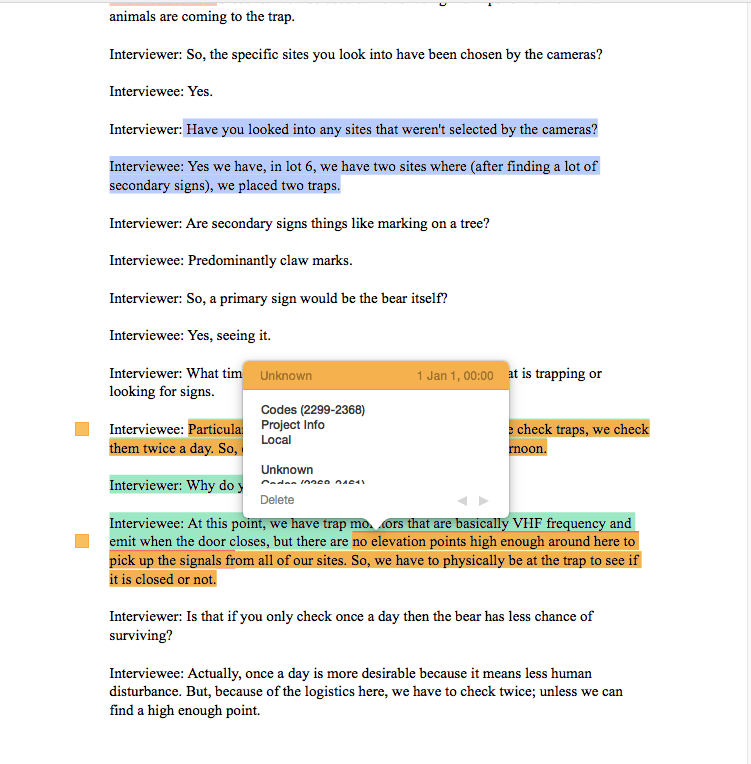
\includegraphics[width=\textwidth]{App/figures/roshan_extract}

\chapter{Repast Parameters File Example}\label{appendix:sims:params}
\begin{lstlisting}[language=XML, caption={Example params.xml file for a Repast simulation}]
<?xml version="1.0" encoding="UTF-8" ?>
<parameters>
  <parameter name="randomSeed" displayName="Default Random Seed" type="int" defaultValue="__NULL__" />
  
  <parameter name="sensingNodeCount" displayName="Number of sensing Nodes" type="int" defaultValue="20" isReadOnly="false" converter="repast.simphony.parameter.StringConverterFactory$IntConverter"  />

  <parameter name="routingNodeCount" displayName="Number of routing Nodes" type="int" defaultValue="4" isReadOnly="false" converter="repast.simphony.parameter.StringConverterFactory$IntConverter" />
  
  <parameter name="centralNodeCount" displayName="Number of central Nodes" type="int" defaultValue="1" isReadOnly="false" converter="repast.simphony.parameter.StringConverterFactory$IntConverter" />
  
  <parameter name="sensingKnowledge" displayName="Knowledge for sensing nodes" type="java.lang.String" defaultValue="MK" isReadOnly="false" converter="repast.simphony.parameter.StringConverterFactory$StringStringConverter"/>

  <parameter name="routingKnowledge" displayName="Knowledge for routing nodes" type="java.lang.String" defaultValue="MK" isReadOnly="false" converter="repast.simphony.parameter.StringConverterFactory$StringStringConverter"/>
  
  <parameter name="centralKnowledge" displayName="Knowledge for central nodes" type="java.lang.String" defaultValue="NK" isReadOnly="false" converter="repast.simphony.parameter.StringConverterFactory$StringStringConverter"/>
  
  <parameter name="captureChance" displayName="chance of image capture" type="double" defaultValue="0.000857703189" isReadOnly="false" converter="repast.simphony.parameter.StringConverterFactory$DoubleConverter"/>
  
  <parameter name="interestingChance" displayName="chance of interesting capture" type="double" defaultValue="0.207" isReadOnly="false" converter="repast.simphony.parameter.StringConverterFactory$DoubleConverter"/>
  
  <parameter name="transRate" displayName="Transmission rate (variable or ideal)" type="java.lang.String" defaultValue="variable" isReadOnly="false" converter="repast.simphony.parameter.StringConverterFactory$StringStringConverter" />
  
  <parameter name="bandwidth" displayName="Chance of image capture (normal or saturated)" type="java.lang.String" defaultValue="normal" isReadOnly="false" converter="repast.simphony.parameter.StringConverterFactory$StringStringConverter" />
  
  <parameter name="hkProcessingTime" displayName="time to process archive" type="int" defaultValue="43" isReadOnly="false" converter="repast.simphony.parameter.StringConverterFactory$IntConverter"/>
  
  <parameter name="mkProcessingTime" displayName="time to process archive" type="int" defaultValue="5" isReadOnly="false" converter="repast.simphony.parameter.StringConverterFactory$IntConverter"/>
  
  <parameter name="tickStop" displayName="Stop at Tick (-1 for No)" type="int" defaultValue="15552000" isReadOnly="false" converter="repast.simphony.parameter.StringConverterFactory$IntConverter"/>
    
  <parameter name="height" displayName="Height" type="int" defaultValue="1200" isReadOnly="false" converter="repast.simphony.parameter.StringConverterFactory$IntConverter" />
  
  <parameter name="width" displayName="Height" type="int" defaultValue="1200" isReadOnly="false" converter="repast.simphony.parameter.StringConverterFactory$IntConverter" />
</parameters>
\end{lstlisting}

\end{appendices}
\backmatter


\end{document}
